%===============================================================================
% LaTeX sjabloon voor de bachelorproef toegepaste informatica aan HOGENT
% Meer info op https://github.com/HoGentTIN/latex-hogent-report
%===============================================================================

\documentclass[dutch,dit,thesis]{hogentreport}

% TODO:
% - If necessary, replace the option `dit`' with your own department!
%   Valid entries are dbo, dbt, dgz, dit, dlo, dog, dsa, soa
% - If you write your thesis in English (remark: only possible after getting
%   explicit approval!), remove the option "dutch," or replace with "english".

\usepackage{lipsum} % For blind text, can be removed after adding actual content
\usepackage{placeins}
\usepackage{listings}
\usepackage{graphics}
\usepackage{biblatex}

%% Pictures to include in the text can be put in the graphics/ folder
\graphicspath{{graphics/}}

%% For source code highlighting, requires pygments to be installed
%% Compile with the -shell-escape flag!
\usepackage[section]{minted}
%% If you compile with the make_thesis.{bat,sh} script, use the following
%% import instead:
%% \usepackage[section,outputdir=../output]{minted}
\usemintedstyle{solarized-light}
\definecolor{bg}{RGB}{253,246,227} %% Set the background color of the codeframe

%% Change this line to edit the line numbering style:
\renewcommand{\theFancyVerbLine}{\ttfamily\scriptsize\arabic{FancyVerbLine}}

%% Macro definition to load external java source files with \javacode{filename}:
\newmintedfile[javacode]{java}{
    bgcolor=bg,
    fontfamily=tt,
    linenos=true,
    numberblanklines=true,
    numbersep=5pt,
    gobble=0,
    framesep=2mm,
    funcnamehighlighting=true,
    tabsize=4,
    obeytabs=false,
    breaklines=true,
    mathescape=false
    samepage=false,
    showspaces=false,
    showtabs =false,
    texcl=false,
}

% Other packages not already included can be imported here

%%---------- Document metadata -------------------------------------------------
% TODO: Replace this with your own information
\author{Colin Callebert}
\supervisor{Dhr. Jan Claes}
\cosupervisor{Dhr. David Vanden Bussche}
\title{Voor- en nadelen van een service-\linebreak architectuur voor bedrijfsapplicaties:\linebreak architecturale overwegingen en best practices}

\academicyear{\advance\year by -1 \the\year--\advance\year by 1 \the\year}
\examperiod{1}
\degreesought{\IfLanguageName{dutch}{Professionele bachelor in de toegepaste informatica}{Bachelor of applied computer science}}
\partialthesis{false} %% To display 'in partial fulfilment'
%\institution{Internshipcompany BVBA.}

%% Add global exceptions to the hyphenation here
\hyphenation{back-slash}

%% The bibliography (style and settings are  found in hogentthesis.cls)
\addbibresource{bachproef.bib}            %% Bibliography file
%\addbibresource{../voorstel/voorstel.bib} %% Bibliography research proposal

%% Prevent empty pages for right-handed chapter starts in twoside mode
\renewcommand{\cleardoublepage}{\clearpage}

\renewcommand{\arraystretch}{1.2}

%% Content starts here.
\begin{document}

%---------- Front matter -------------------------------------------------------

\frontmatter

\hypersetup{pageanchor=false} %% Disable page numbering references
%% Render a Dutch outer title page if the main language is English
\IfLanguageName{english}{%
    %% If necessary, information can be changed here
    \degreesought{Professionele Bachelor toegepaste informatica}%
    \begin{otherlanguage}{dutch}%
       \maketitle%
    \end{otherlanguage}%
}{}

%% Generates title page content
\maketitle
\hypersetup{pageanchor=true}

%%=============================================================================
%% Voorwoord
%%=============================================================================

\chapter*{\IfLanguageName{dutch}{Woord vooraf}{Preface}}%
\label{ch:voorwoord}

%% TODO:
%% Het voorwoord is het enige deel van de bachelorproef waar je vanuit je
%% eigen standpunt (``ik-vorm'') mag schrijven. Je kan hier bv. motiveren
%% waarom jij het onderwerp wil bespreken.
%% Vergeet ook niet te bedanken wie je geholpen/gesteund/... heeft
In deze bachelorproef onderzoek ik de voor- en nadelen van microservices ten opzichte van monolithische applicaties. Dit onderwerp sprak mij om verschillende redenen aan. Ten eerste ben ik geïnteresseerd in het ontwikkelen van applicaties en het optimaliseren van hun prestaties. Ten tweede ben ik ook gefascineerd door de verschillende architectuurkeuzes die mogelijk zijn bij het ontwikkelen van applicaties. Ten slotte vind ik het verkennen en leren van nieuwe technologieën een boeiende en plezierige ervaring.


Tijdens mijn stage bij Cloudway, een bedrijf gericht op de cloud, draaide mijn project volledig in de cloud en maakte het gebruik van microservices. Deze praktijkervaring gaf mij diepgaande inzichten in hoe microservices in de praktijk worden toegepast en welke uitdagingen en voordelen ze met zich meebrengen. Het stelde mij in staat om theoretische kennis direct toe te passen en te testen in een professionele omgeving, wat mijn begrip en interesse in dit onderwerp verder versterkte.


Graag wil ik mijn co-promotor, David Vanden Bussche, bedanken voor zijn begeleiding en waardevolle feedback gedurende het schrijven van deze bachelorproef. Zijn expertise en geduld hebben een cruciale rol gespeeld in het succesvol afronden van dit onderzoek. 


Tot slot wil ik mijn familie en vrienden bedanken voor hun onvoorwaardelijke steun en motivatie gedurende deze periode. Hun aanmoedigingen en begrip hebben mij geholpen om dit onderzoek met succes af te ronden. Ik hoop dat deze bachelorproef een nuttige bron van informatie zal zijn voor studenten, ontwikkelaars en IT-beheerders die meer willen weten over de impact van microservices op de ontwikkeling en het beheer van bedrijfsapplicaties. Ik wens u veel leesplezier en hoop dat de inzichten en best practices die in dit werk worden gepresenteerd, waardevol zullen blijken in uw eigen professionele praktijk.

%%=============================================================================
%% Samenvatting
%%=============================================================================

% TODO: De "abstract" of samenvatting is een kernachtige (~ 1 blz. voor een
% thesis) synthese van het document.
%
% Een goede abstract biedt een kernachtig antwoord op volgende vragen:
%
% 1. Waarover gaat de bachelorproef?
% 2. Waarom heb je er over geschreven?
% 3. Hoe heb je het onderzoek uitgevoerd?
% 4. Wat waren de resultaten? Wat blijkt uit je onderzoek?
% 5. Wat betekenen je resultaten? Wat is de relevantie voor het werkveld?
%
% Daarom bestaat een abstract uit volgende componenten:
%
% - inleiding + kaderen thema
% - probleemstelling
% - (centrale) onderzoeksvraag
% - onderzoeksdoelstelling
% - methodologie
% - resultaten (beperk tot de belangrijkste, relevant voor de onderzoeksvraag)
% - conclusies, aanbevelingen, beperkingen
%
% LET OP! Een samenvatting is GEEN voorwoord!

%%---------- Nederlandse samenvatting -----------------------------------------
%
% TODO: Als je je bachelorproef in het Engels schrijft, moet je eerst een
% Nederlandse samenvatting invoegen. Haal daarvoor onderstaande code uit
% commentaar.
% Wie zijn bachelorproef in het Nederlands schrijft, kan dit negeren, de inhoud
% wordt niet in het document ingevoegd.

\IfLanguageName{english}{%
\selectlanguage{dutch}
\chapter*{Samenvatting}
\selectlanguage{english}
}{}

%%---------- Samenvatting -----------------------------------------------------
% De samenvatting in de hoofdtaal van het document

\chapter*{\IfLanguageName{dutch}{Samenvatting}{Abstract}}
Bij een monolithische architectuur wordt de volledige applicatie als één enkel geheel met een eigen codebase en infrastructuur ontwikkeld. In een microservicesarchitectuur wordt de functionaliteit opgesplitst in kleinere, zelfstandig werkende services, die elk hun eigen codebase en infrastructuur gebruiken. Het is cruciaal om bij het kiezen van een architectuur rekening te houden met de specifieke behoeften van de applicatie en de bedrijfsdoelstellingen. Microservices kunnen de ontwikkelingstijd versnellen en de complexiteit van de applicatie verminderen, terwijl een monolithische architectuur beter geschikt kan zijn voor minder complexe applicaties die minder onderhoud vereisen.


Bij het implementeren van microservices zijn aspecten zoals load balancing, service discovery, netwerkbeveiliging en weerbaarheid essentieel om de schaalbaarheid en prestaties te garanderen. Servicemeshes bieden functionaliteit om deze uitdagingen aan te pakken. Bij het opzetten van een servicemesh voor bedrijfsapplicaties is het belangrijk om architecturale overwegingen en best practices te volgen om optimale schaalbaarheid en prestaties te bereiken.


Dit onderzoek richt zich op het bepalen van de geschikte architectuurkeuze voor een specifieke situatie, aan de hand van een case study. Hierbij worden de voor- en nadelen van zowel monolithische als microservicesarchitecturen belicht. Eerst wordt een monolithische applicatie opgezet, waarna deze wordt opgesplitst in microservices. De prestaties van beide architecturen worden vervolgens getest en geanalyseerd. De resultaten van dit onderzoek kunnen bijdragen aan het optimaliseren van applicatieontwikkeling en -prestaties.


Deze bachelorproef biedt een vergelijking tussen monolithische en microservicesarchitecturen, met een focus op de praktische toepassingen en de impact op bedrijfsapplicaties. Door de resultaten van de case study en de opgedane inzichten kunnen organisaties beter geïnformeerde beslissingen nemen over welke architectuur het beste aansluit bij hun specifieke behoeften en doelstellingen. 


In deze context onderzochten we de verschillende aspecten van beide architecturen, waaronder de operationele complexiteit, schaalbaarheid, onderhoudbaarheid en de prestaties. De bevindingen uit dit onderzoek geven een duidelijk beeld van de voordelen en uitdagingen van het gebruik van microservices in vergelijking met een monolithische benadering. Dit kan organisaties helpen om strategische keuzes te maken die hun IT-infrastructuur en applicatiebeheer verbeteren.


De samenvatting geeft een overzicht van de belangrijkste bevindingen en aanbevelingen die voortkomen uit het onderzoek. Het biedt waardevolle inzichten voor ontwikkelaars, IT-beheerders en besluitvormers die overwegen om de transitie naar een microservicesarchitectuur te maken. De resultaten tonen aan dat, hoewel de overstap naar microservices aanzienlijke voordelen biedt, er ook uitdagingen zijn die zorgvuldig moeten worden beheerd om de voordelen volledig te kunnen benutten.


%---------- Inhoud, lijst figuren, ... -----------------------------------------

\tableofcontents

% In a list of figures, the complete caption will be included. To prevent this,
% ALWAYS add a short description in the caption!
%
%  \caption[short description]{elaborate description}
%
% If you do, only the short description will be used in the list of figures

\listoffigures

% If you included tables and/or source code listings, uncomment the appropriate
% lines.
%\listoftables
%\listoflistings

% Als je een lijst van afkortingen of termen wil toevoegen, dan hoort die
% hier thuis. Gebruik bijvoorbeeld de ``glossaries'' package.
% https://www.overleaf.com/learn/latex/Glossaries

%---------- Kern ---------------------------------------------------------------

\mainmatter{}

% De eerste hoofdstukken van een bachelorproef zijn meestal een inleiding op
% het onderwerp, literatuurstudie en verantwoording methodologie.
% Aarzel niet om een meer beschrijvende titel aan deze hoofdstukken te geven of
% om bijvoorbeeld de inleiding en/of stand van zaken over meerdere hoofdstukken
% te verspreiden!

%%=============================================================================
%% Inleiding
%%=============================================================================

\chapter{\IfLanguageName{dutch}{Inleiding}{Introduction}}%
\label{ch:inleiding}

\section{\IfLanguageName{dutch}{Probleemstelling}{Problem Statement}}%
\label{sec:probleemstelling}

De complexiteit van moderne bedrijfsapplicaties groeit voortdurend, wat heeft geleid tot de opkomst van verschillende architecturale benaderingen om aan deze behoeften te voldoen. Eén van de belangrijkste overwegingen bij het ontwikkelen van een applicatie is de keuze tussen een monolithische architectuur en een microservicesarchitectuur. Bij een monolithische architectuur wordt de volledige applicatie als één enkel geheel met een centrale codebase en infrastructuur ontwikkeld. Deze aanpak is over het algemeen eenvoudiger te implementeren en te beheren, maar kan problematisch worden naarmate de applicatie groter en complexer wordt. Monolithische architecturen kunnen leiden tot problemen met onderhoud, schaalbaarheid en flexibiliteit doordat alle functionaliteit binnen één enkele codebase wordt ondergebracht.


Daartegenover staat de microservicesarchitectuur, waarbij de functionaliteit wordt opgesplitst in kleinere, onafhankelijke services. Elke service heeft zijn eigen codebase en infrastructuur, wat voordelen biedt zoals verbeterde schaalbaarheid, onderhoudbaarheid en flexibiliteit. Echter, deze aanpak introduceert ook nieuwe complexiteiten, met name op het gebied van communicatie en coördinatie tussen de verschillende services.


In dit onderzoek richten we ons op een specifieke casus: een applicatie voor een boerderij. Deze applicatie omvat verschillende functionaliteiten, zoals het inloggen/registreren, het maken van afspraken, gegevens wijzigen en het beheren van de afspraken. De huidige implementatie van deze applicatie volgt een monolithische architectuur en is gebouwd met behulp van JavaScript.


Om de mogelijkheden van schaalbaarheid en prestatieverbetering verder te verkennen, willen we onderzoeken hoe deze applicatie zou kunnen profiteren van een microservicesarchitectuur. We zullen de functionaliteiten van de applicatie opsplitsen in verschillende microservices, zoals registreren, activiteiten en gebruiker. Deze microservices zouden dan via een servicemesh worden beheerd en met elkaar communiceren.


Daarnaast zullen we ook aandacht besteden aan de implementatie-uitdagingen die gepaard gaan met de overgang van een monolithische naar een microservicesarchitectuur. Dit omvat het omgaan met aspecten zoals service discovery, load balancing, netwerkbeveiliging en weerbaarheid. We willen inzicht krijgen in hoe een servicemesh kan bijdragen aan het oplossen van deze uitdagingen en het verbeteren van de algehele prestaties en schaalbaarheid van de applicatie.


Verder zullen we onderzoeken welke impact deze overgang heeft op de ontwikkelingsprocessen en de operationele praktijken binnen het team. Dit omvat de leercurve voor ontwikkelaars, de complexiteit van het testen en debuggen van microservices, en de noodzaak voor effectieve monitoring en logging.
Dit onderzoek beoogt inzicht te verschaffen in de belangrijkste architecturale overwegingen en best practices bij het gebruik van een servicemesh om schaalbaarheid en prestaties te bereiken in bedrijfsapplicaties. We zullen de voordelen, uitdagingen en mogelijke impact van een dergelijke architectuurverandering voor de applicatie onderzoeken. Daarnaast zullen we deze bevindingen vergelijken met de huidige monolithische implementatie om de verschillen en mogelijke voordelen duidelijk te identificeren.


\section{\IfLanguageName{dutch}{Onderzoeksvraag}{Research question}}%
\label{sec:onderzoeksvraag}
Voor- en nadelen van een service-   architectuur voor bedrijfsapplicaties: architecturale overwegingen en best practices

\section{\IfLanguageName{dutch}{Onderzoeksdoelstelling}{Research objective}}%
\label{sec:onderzoeksdoelstelling}

Het beoogde resultaat van deze bachelorproef is het verschaffen van inzicht in de voordelen en nadelen van een monolithische architectuur tegenover een microservices architectuur. Het succes van dit onderzoek wordt bepaald door het identificeren van de belangrijkste architecturale overwegingen, uitdagingen en het evalueren van de mogelijke verbeteringen in schaalbaarheid en prestaties.

\section{\IfLanguageName{dutch}{Opzet van deze bachelorproef}{Structure of this bachelor thesis}}%
\label{sec:opzet-bachelorproef}

% Het is gebruikelijk aan het einde van de inleiding een overzicht te
% geven van de opbouw van de rest van de tekst. Deze sectie bevat al een aanzet
% die je kan aanvullen/aanpassen in functie van je eigen tekst.

De rest van deze bachelorproef is als volgt opgebouwd:

In Hoofdstuk~\ref{ch:stand-van-zaken} wordt een overzicht gegeven van de stand van zaken binnen het onderzoeksdomein, op basis van een literatuurstudie.

In Hoofdstuk~\ref{ch:methodologie} wordt de methodologie toegelicht en worden de gebruikte onderzoekstechnieken besproken om een antwoord te kunnen formuleren op de onderzoeksvragen.

In Hoofdstuk~\ref{ch:keuze-software} wordt de software besproken die gebruikt werd om de microservices architectuur op te zetten en te implementeren.

In Hoofdstuk~\ref{ch:monoliet} wordt de huidige monolithische architectuur van de applicatie besproken en wordt de implementatie van deze architectuur toegelicht.

In Hoofdstuk~\ref{ch:opsplitsen-backend} wordt de opsplitsing en herstructurering van de backend van de applicatie besproken en wordt de implementatie van deze architectuur toegelicht.

In Hoofdstuk~\ref{ch:docker-backend} wordt de opgesplitste backend van de applicatie in Docker-containers geplaatst en wordt de implementatie van deze architectuur toegelicht.

In Hoofdstuk~\ref{ch:implementatie-backend-istio} wordt de implementatie van de services in Isto besproken en wordt de implementatie van deze architectuur toegelicht.

In Hoofdstuk~\ref{ch:testen-prestatieanalyse} worden de prestaties van monoliet en microservices architectuur getest en geanalyseerd.

% TODO: Vul hier aan voor je eigen hoofstukken, één of twee zinnen per hoofdstuk

In Hoofdstuk~\ref{ch:conclusie}, ten slotte, wordt de conclusie gegeven en een antwoord geformuleerd op de onderzoeksvragen. Daarbij wordt ook een aanzet gegeven voor toekomstig onderzoek binnen dit domein.
\chapter{\IfLanguageName{dutch}{Stand van zaken}{State of the art}}%
\label{ch:stand-van-zaken}

% Tip: Begin elk hoofdstuk met een paragraaf inleiding die beschrijft hoe
% dit hoofdstuk past binnen het geheel van de bachelorproef. Geef in het
% bijzonder aan wat de link is met het vorige en volgende hoofdstuk.

% Pas na deze inleidende paragraaf komt de eerste sectiehoofding.

Dit hoofdstuk bevat je literatuurstudie. De inhoud gaat verder op de inleiding, maar zal het onderwerp van de bachelorproef *diepgaand* uitspitten. De bedoeling is dat de lezer na lezing van dit hoofdstuk helemaal op de hoogte is van de huidige stand van zaken (state-of-the-art) in het onderzoeksdomein. Iemand die niet vertrouwd is met het onderwerp, weet nu voldoende om de rest van het verhaal te kunnen volgen, zonder dat die er nog andere informatie moet over opzoeken \autocite{Pollefliet2011}.

Je verwijst bij elke bewering die je doet, vakterm die je introduceert, enz.\ naar je bronnen. In \LaTeX{} kan dat met het commando \texttt{$\backslash${textcite\{\}}} of \texttt{$\backslash${autocite\{\}}}. Als argument van het commando geef je de ``sleutel'' van een ``record'' in een bibliografische databank in het Bib\LaTeX{}-formaat (een tekstbestand). Als je expliciet naar de auteur verwijst in de zin (narratieve referentie), gebruik je \texttt{$\backslash${}textcite\{\}}. Soms is de auteursnaam niet expliciet een onderdeel van de zin, dan gebruik je \texttt{$\backslash${}autocite\{\}} (referentie tussen haakjes). Dit gebruik je bv.~bij een citaat, of om in het bijschrift van een overgenomen afbeelding, broncode, tabel, enz. te verwijzen naar de bron. In de volgende paragraaf een voorbeeld van elk.

\textcite{Knuth1998} schreef een van de standaardwerken over sorteer- en zoekalgoritmen. Experten zijn het erover eens dat cloud computing een interessante opportuniteit vormen, zowel voor gebruikers als voor dienstverleners op vlak van informatietechnologie~\autocite{Creeger2009}.

Let er ook op: het \texttt{cite}-commando voor de punt, dus binnen de zin. Je verwijst meteen naar een bron in de eerste zin die erop gebaseerd is, dus niet pas op het einde van een paragraaf.

\lipsum[7-20]

%%=============================================================================
%% Methodologie
%%=============================================================================

\chapter{\IfLanguageName{dutch}{Methodologie}{Methodology}}%
\label{ch:methodologie}

%% TODO: In dit hoofstuk geef je een korte toelichting over hoe je te werk bent
%% gegaan. Verdeel je onderzoek in grote fasen, en licht in elke fase toe wat
%% de doelstelling was, welke deliverables daar uit gekomen zijn, en welke
%% onderzoeksmethoden je daarbij toegepast hebt. Verantwoord waarom je
%% op deze manier te werk gegaan bent.
%% 
%% Voorbeelden van zulke fasen zijn: literatuurstudie, opstellen van een
%% requirements-analyse, opstellen long-list (bij vergelijkende studie),
%% selectie van geschikte tools (bij vergelijkende studie, "short-list"),
%% opzetten testopstelling/PoC, uitvoeren testen en verzamelen
%% van resultaten, analyse van resultaten, ...
%%
%% !!!!! LET OP !!!!!
%%
%% Het is uitdrukkelijk NIET de bedoeling dat je het grootste deel van de corpus
%% van je bachelorproef in dit hoofstuk verwerkt! Dit hoofdstuk is eerder een
%% kort overzicht van je plan van aanpak.
%%
%% Maak voor elke fase (behalve het literatuuronderzoek) een NIEUW HOOFDSTUK aan
%% en geef het een gepaste titel.

Om de onderzoeksvraag te beantwoorden, werden de volgende stappen gevolgd:

\begin{itemize}
  \item Voorstudie
  \item Implementatie
  \item Analyse
\end{itemize} 

Het opzetten van de microservices architectuur zal gebeuren door de monolithische architectuur van de ouderenboerderijapplicatie op te splitsen in verschillende services. 
\begin{enumerate}
	\item \textbf{Opzetten van monolithische architectuur:} In deze fase zal ik de ouderenboerderijapplicatie opzetten als een monolithische architectuur. Dit omvat het gebruik van Node.js en React om een toepassing te creëren die een MySQL-database aanroept. De applicatie zal een inlogsysteem, een profielpagina en de mogelijkheid om zich te registreren voor activiteiten bevatten. Deze toepassing bestaat uit een backend en een frontend en draait lokaal op twee verschillende poorten.
	\item \textbf{Opsplitsen en herstructureren van de backend:} De volgende stap is het opsplitsen en herstructureren van de backend naar drie verschillende services. Een van de voordelen van microservices is dat elke capability kan gebouwd worden in de technologie die er best voor geschikt is. Het gebruikersgedeelte wordt omgezet van Node.js naar Python en zal zijn gegevens ophalen uit een MongoDB-database. Het activiteitengedeelte blijft in Node.js en zal zijn gegevens ophalen uit een MongoDB-database. Het registratiegedeelte blijft in Node.js en zal zijn gegevens blijven ophalen uit een MySQL-database. Elk van deze services zal op een aparte poort draaien.
	\item \textbf{Draaien van backend in Docker containers:} Vervolgens zullen de drie backend services in Docker-containers worden geplaatst. Deze containers zullen onderling communiceren en communiceren met de databases.
	\item \textbf{Implementatie van de drie backend services in Istio:} De drie backend services worden in containers geplaatst en geïmplementeerd in Istio. Hierdoor kunnen ze communiceren met de frontend en met elkaar.
	\item \textbf{Testen en prestatieanalyse:} Tot slot zal ik de prestaties van de applicatie testen en meten. Dit omvat het uitvoeren van verschillende tests en het meten van de prestaties van de applicatie. Er zal ook worden nagekeken wat het effect is van de functionaliteiten die door de servicemesh geboden worden.
\end{enumerate}




% Voeg hier je eigen hoofdstukken toe die de ``corpus'' van je bachelorproef
% vormen. De structuur en titels hangen af van je eigen onderzoek. Je kan bv.
% elke fase in je onderzoek in een apart hoofdstuk bespreken.

%\input{...}
%\input{...}
%...

\chapter*{\IfLanguageName{dutch}{Keuze software}{Software choice}}%
\label{ch:keuze-software}

\subsection*{Istio}
Istio is een open-source servicemesh die het beheer van microservices in een Kubernetes cluster vereenvoudigt. Het biedt een uniforme manier om de communicatie tussen services te beveiligen, te beheren en te monitoren. Het is platformonafhankelijk en kan worden geïntegreerd met verschillende Kubernetes-distributies. Istio is een van de meest populaire servicemeshes en wordt ondersteund door grote bedrijven zoals Google, IBM en Red Hat. Het is een volwassen project met een actieve community en een snelgroeiend ecosysteem \autocite{Istio}. 

Bovenstaande redenen en de prijs (gratis) hebben mij doen besluiten om Istio te gebruiken voor het beheren van de microservices in mijn applicatie. 

Voor het opzetten en beheren van de Kubernetes cluster heb ik gekozen voor Minikube. Minikube is een tool die het mogelijk maakt om een lokale Kubernetes cluster te draaien op een enkele docker container. Het is eenvoudig te installeren en te gebruiken en biedt een snelle manier om te experimenteren met Kubernetes en Istio. Minikube is ideaal voor het ontwikkelen en testen van microservices op een lokale machine \autocite{Minikube}. Kubernetes biedt autoscaling fuctionaliteit. Autoscaling is een mechanisme dat automatisch het aantal replica’s van een pod aanpast op basis van de huidige belasting en het gebruik van resources. Dit helpt om applicaties schaalbaar te maken en optimaal gebruik te maken van beschikbare resources, waardoor prestaties worden verbeterd en kosten worden beheerst \autocite{Kubernetes}.


In de bijlage \ref{ch:software} is een handleiding te vinden over hoe Istio geïnstalleerd kan worden en hoe het voor de eerste keer gebruikt kan worden.

\subsection*{Monoliet applicatie}
Voor de monoliet applicatie heb ik gekozen voor een combinatie van Node.js en React. Node.js is een JavaScript runtime die het mogelijk maakt om JavaScript code uit te voeren op de server. Het is lichtgewicht, efficiënt en schaalbaar, waardoor het ideaal is voor het bouwen van webapplicaties. React is een JavaScript-bibliotheek voor het bouwen van gebruikersinterfaces \autocite{Nodejs} \autocite{React}.

Deze combinatie van technologieën is populair en wordt veel gebruikt in de industrie. Het biedt een goede balans tussen prestaties, productiviteit en flexibiliteit. Bovendien zijn er veel bibliotheken en frameworks beschikbaar die het ontwikkelen van webapplicaties met Node.js en React vereenvoudigen.

De data wordt opgeslagen in een MySQL-database en de communicatie tussen de frontend en de backend gebeurt via API-calls met axios. Dit is een eenvoudige en gestroomlijnde manier om gegevens uit te wisselen tussen de verschillende delen van de applicatie \autocite{MySQL} \autocite{Axios}. 

\subsection*{Microservices}
Microservices geven de mogelijkheid om de applicatie op te splitsen in kleinere en onafhankelijke services. Dit geeft de developper de mogelijkheid om elke service te ontwikkelen in de technologie die er best voor geschikt is. Voor de microservices is er gekozen voor Python en Node.js. Python is een veelzijdige programmeertaal die wordt gebruikt voor het ontwikkelen van webapplicaties, data-analyse, machine learning en nog veel meer. Het is eenvoudig te leren en heeft een grote community en een uitgebreide set bibliotheken en frameworks \autocite{Python}. Node.js is een JavaScript runtime die het mogelijk maakt om JavaScript code uit te voeren op de server. Het is lichtgewicht, efficiënt en schaalbaar, waardoor het ideaal is voor het bouwen van webapplicaties \autocite{Nodejs}. Zowel Python als Node.js zijn uitstekend geschikt voor containergebaseerde applicaties vanwege hun leesbaarheid, rijke ecosystemen, ondersteuning voor microservices en gemakkelijke integratie met containerization tools. Ze bieden ontwikkelaars de middelen om snel en efficiënt robuuste, schaalbare en onderhoudbare applicaties te bouwen en te beheren.


De data kan ook opgeslagen worden in verschillende soorten databases. Voor de gebruikersservice en de activiteitenservice is er gekozen voor een MongoDB- database. MongoDB is een NoSQL-database die bekend staat om zijn flexibiliteit en schaalbaarheid. Het is ideaal voor het opslaan van ongestructureerde gegevens en het verwerken van grote hoeveelheden gegevens. Voor de registratieservice is er gekozen voor een MySQL-database. MySQL is een relationele database die bekend staat om zijn robuuste transactiemogelijkheden en uitstekende ondersteuning voor relationele gegevensmodellering \autocite{MongoDB} \autocite{MySQL}.


\chapter{\IfLanguageName{dutch}{Opzetten van monolitische architectuur}{Setting up monolithic architecture}}
\label{ch:monoliet}
Er wordt begonnen met het opzetten van een ouderenboerderijapplicatie die een monolithische architectuur volgt, waarbij alle functionaliteiten zich binnen één enkele backend bevinden, wat zowel voordelen als beperkingen met zich meebrengt. In deze initiële opzet functioneert zowel de backend als de frontend elk op afzonderlijke poorten, met de backend volledig ontwikkeld in Node.js en de frontend in React. De communicatie tussen de backend en de MySQL-database gebeurt met Knex, terwijl de frontend via Axios API-calls met de backend communiceert, wat een gestroomlijnde interactie tussen de verschillende delen van de applicatie mogelijk maakt.

\begin{figure}[H]
	\centering	
	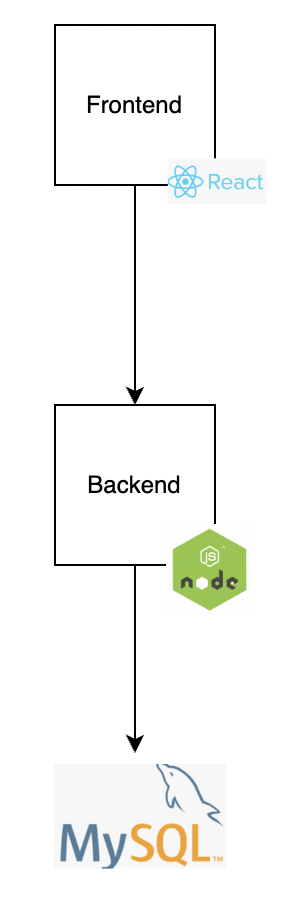
\includegraphics[width = 3cm]{monoliet.png} 
	\caption{Architectuur monolitische applicatie} 
	\label{fig:monolietBP} 
\end{figure}
\FloatBarrier


De functionaliteiten van de applicatie omvatten een auth0 inlogsysteem, een gebruikersprofielpagina en de mogelijkheid voor gebruikers om zich te registreren voor verschillende activiteiten. 

Bij het laden van de applicatie krijgt de gebruiker de homepagina te zien, waar hij wat infomatie over de boerderij en de activiteieten kan vinden.

\begin{figure}[H]
    \centering	
    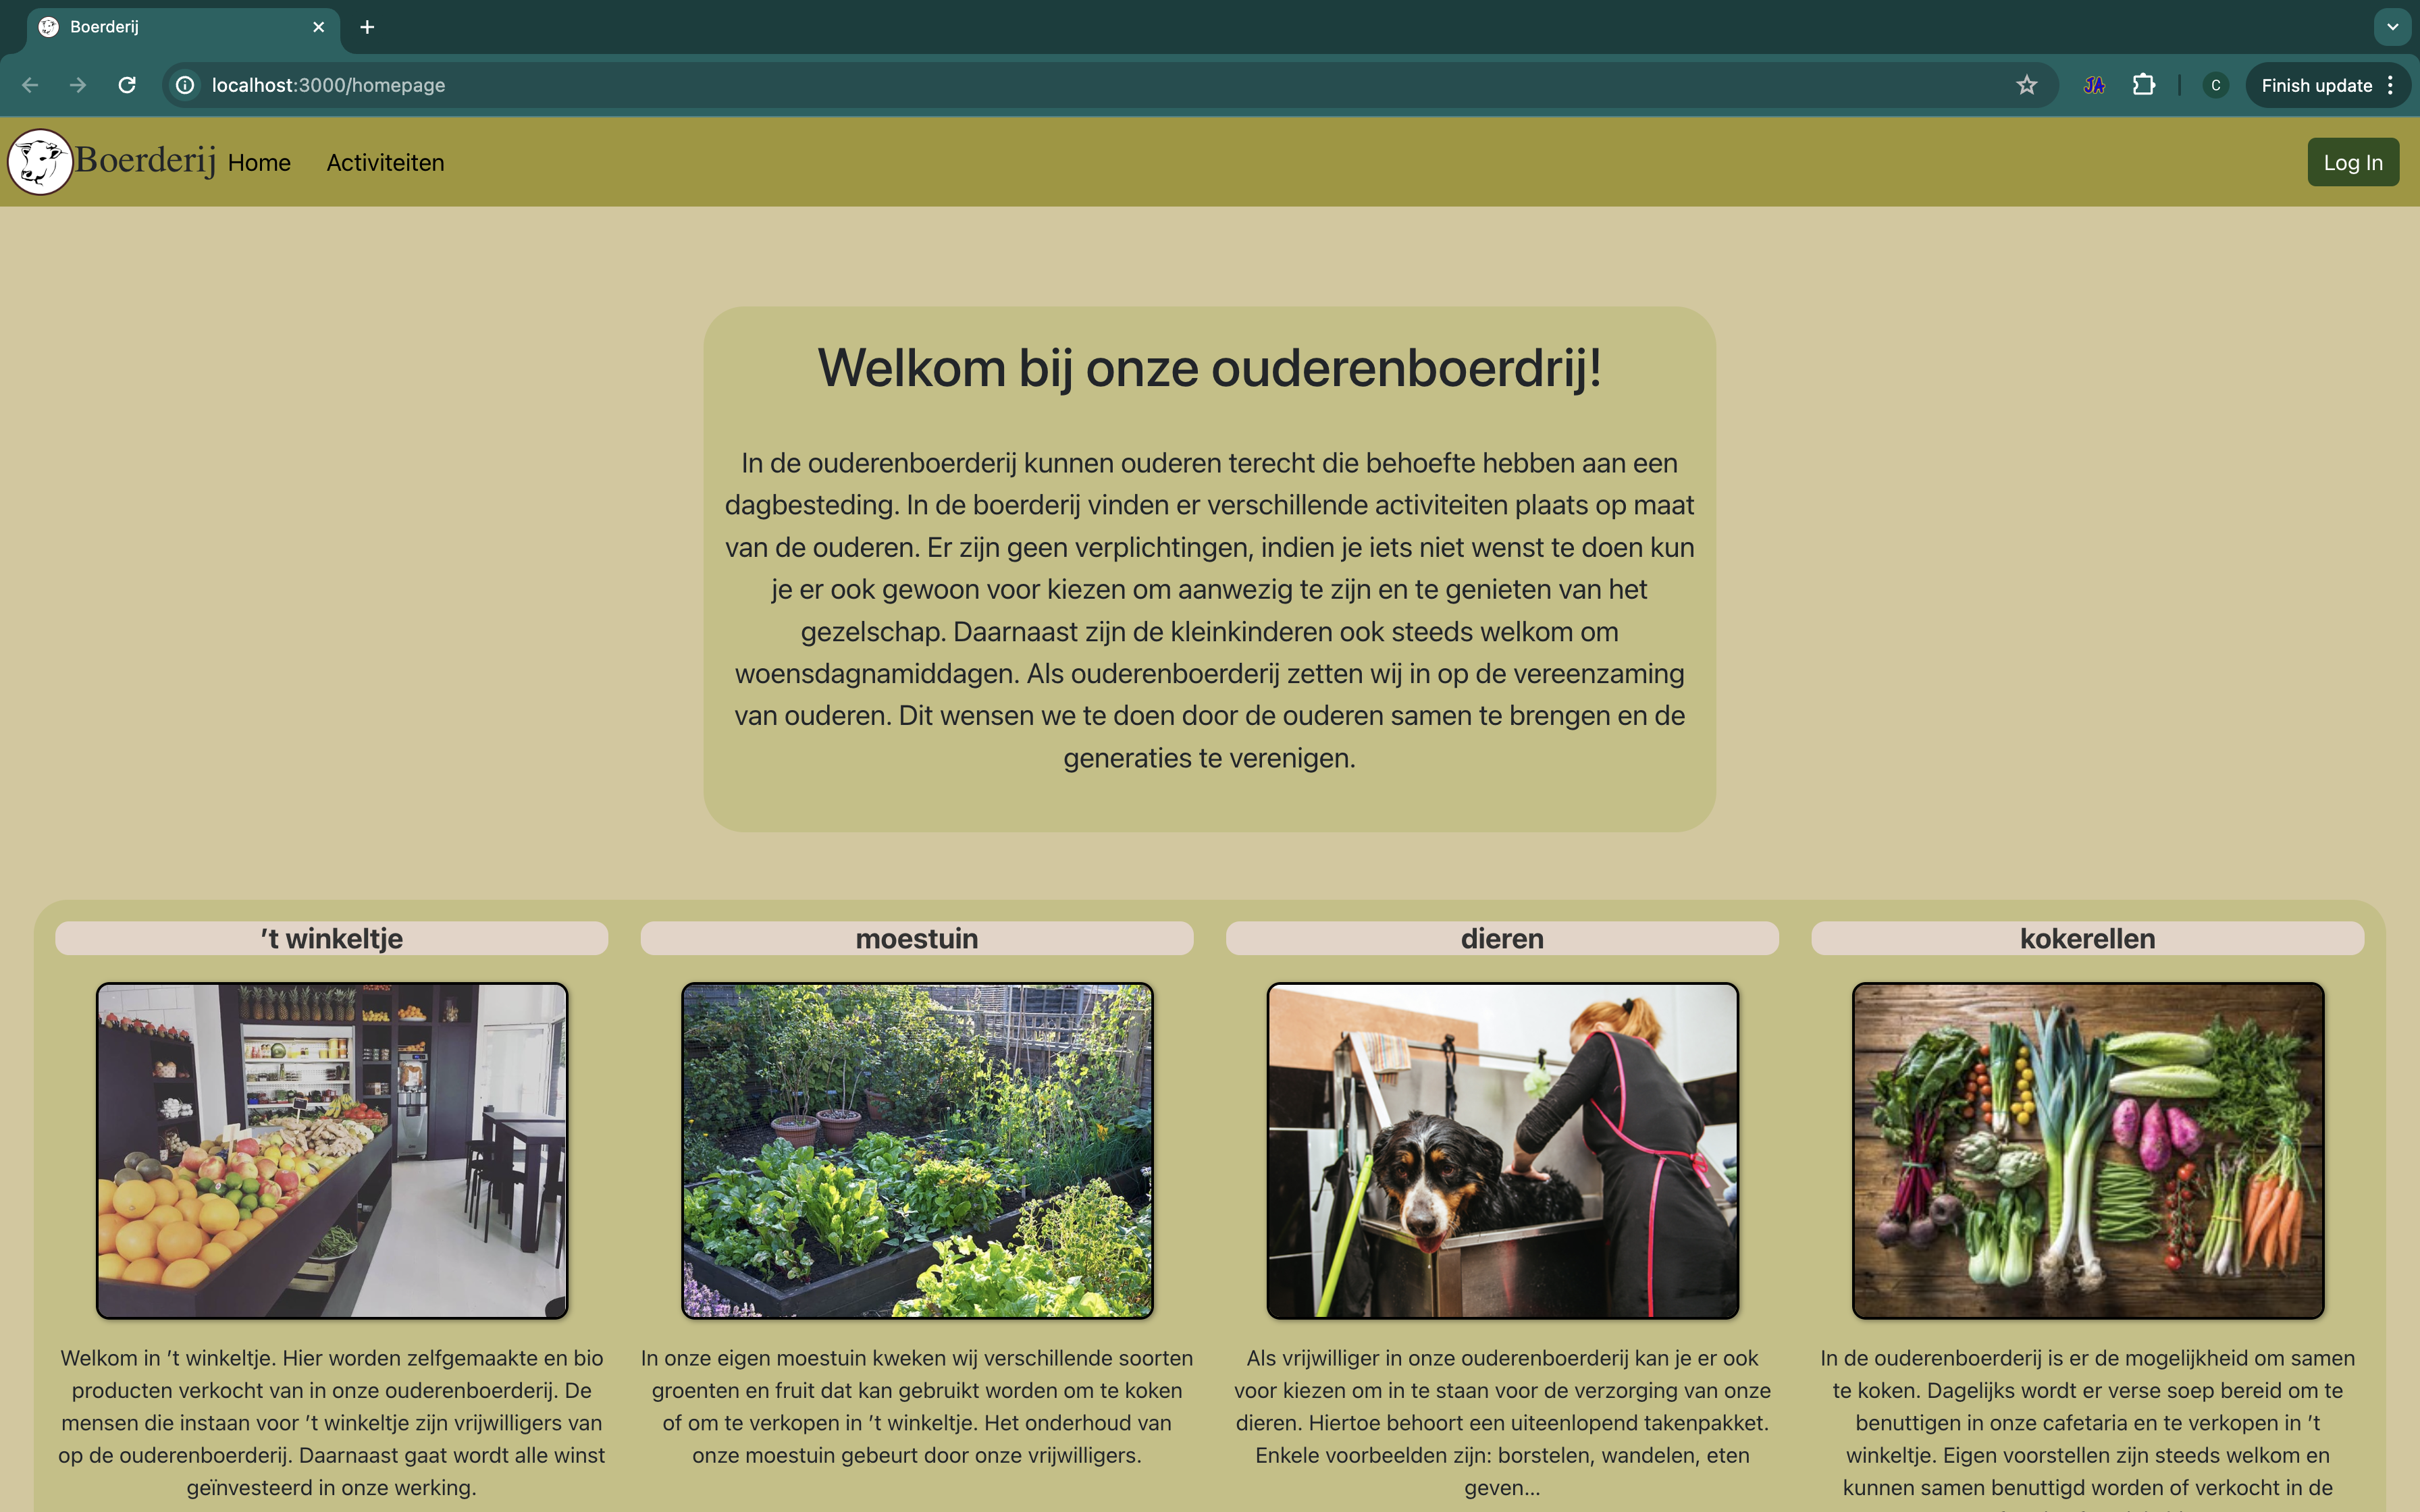
\includegraphics[width = 14cm]{Homescreen.png} 
    \caption{Homepagina} 
    \label{fig:home}
\end{figure}

Vanaf de homepagina kan de gebruiker zich inloggen of registreren. Na het inloggen krijgt de gebruiker toegang tot zijn profielpagina waar hij zijn gegevens kan aanpassen 

\begin{figure}[H]
    \centering	
    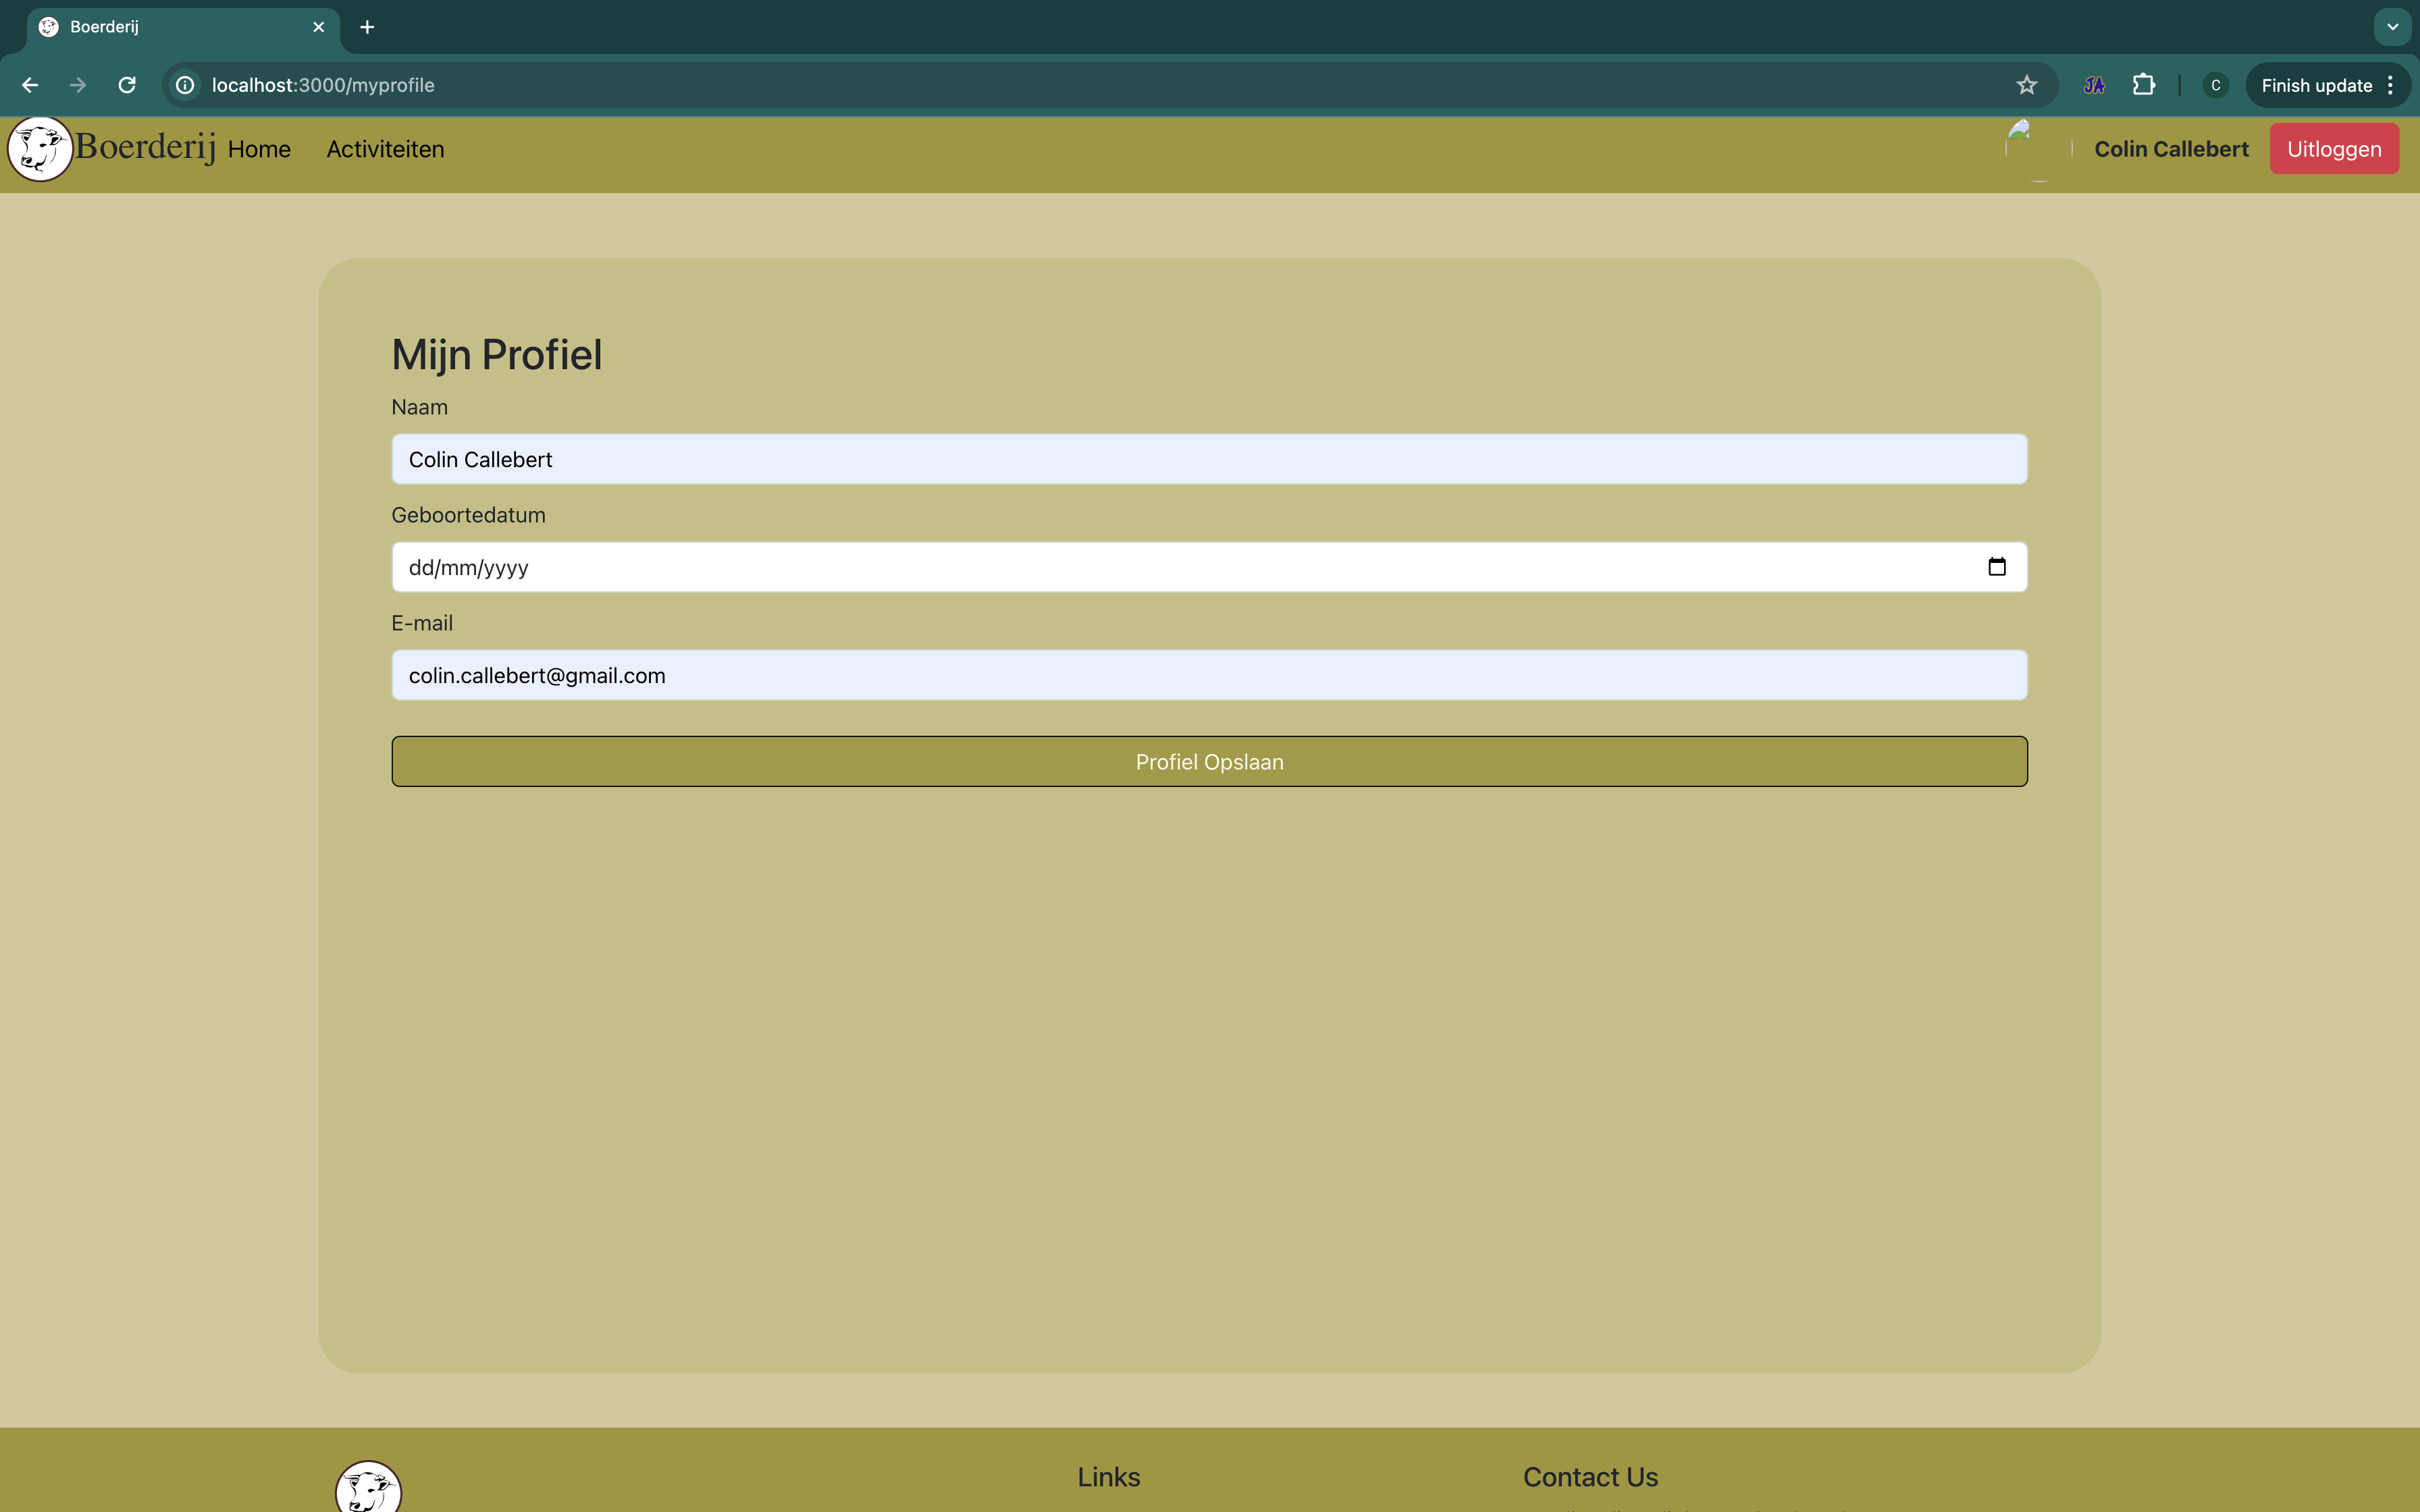
\includegraphics[width = 14cm]{Profiel.png} 
    \caption{Profielpagina} 
    \label{fig:profile}
\end{figure}

De gebruiker kan zich ook registreren voor activiteiten. De activiteiten worden weergegeven op de activiteitenpagina.

\begin{figure}[H]
    \centering	
    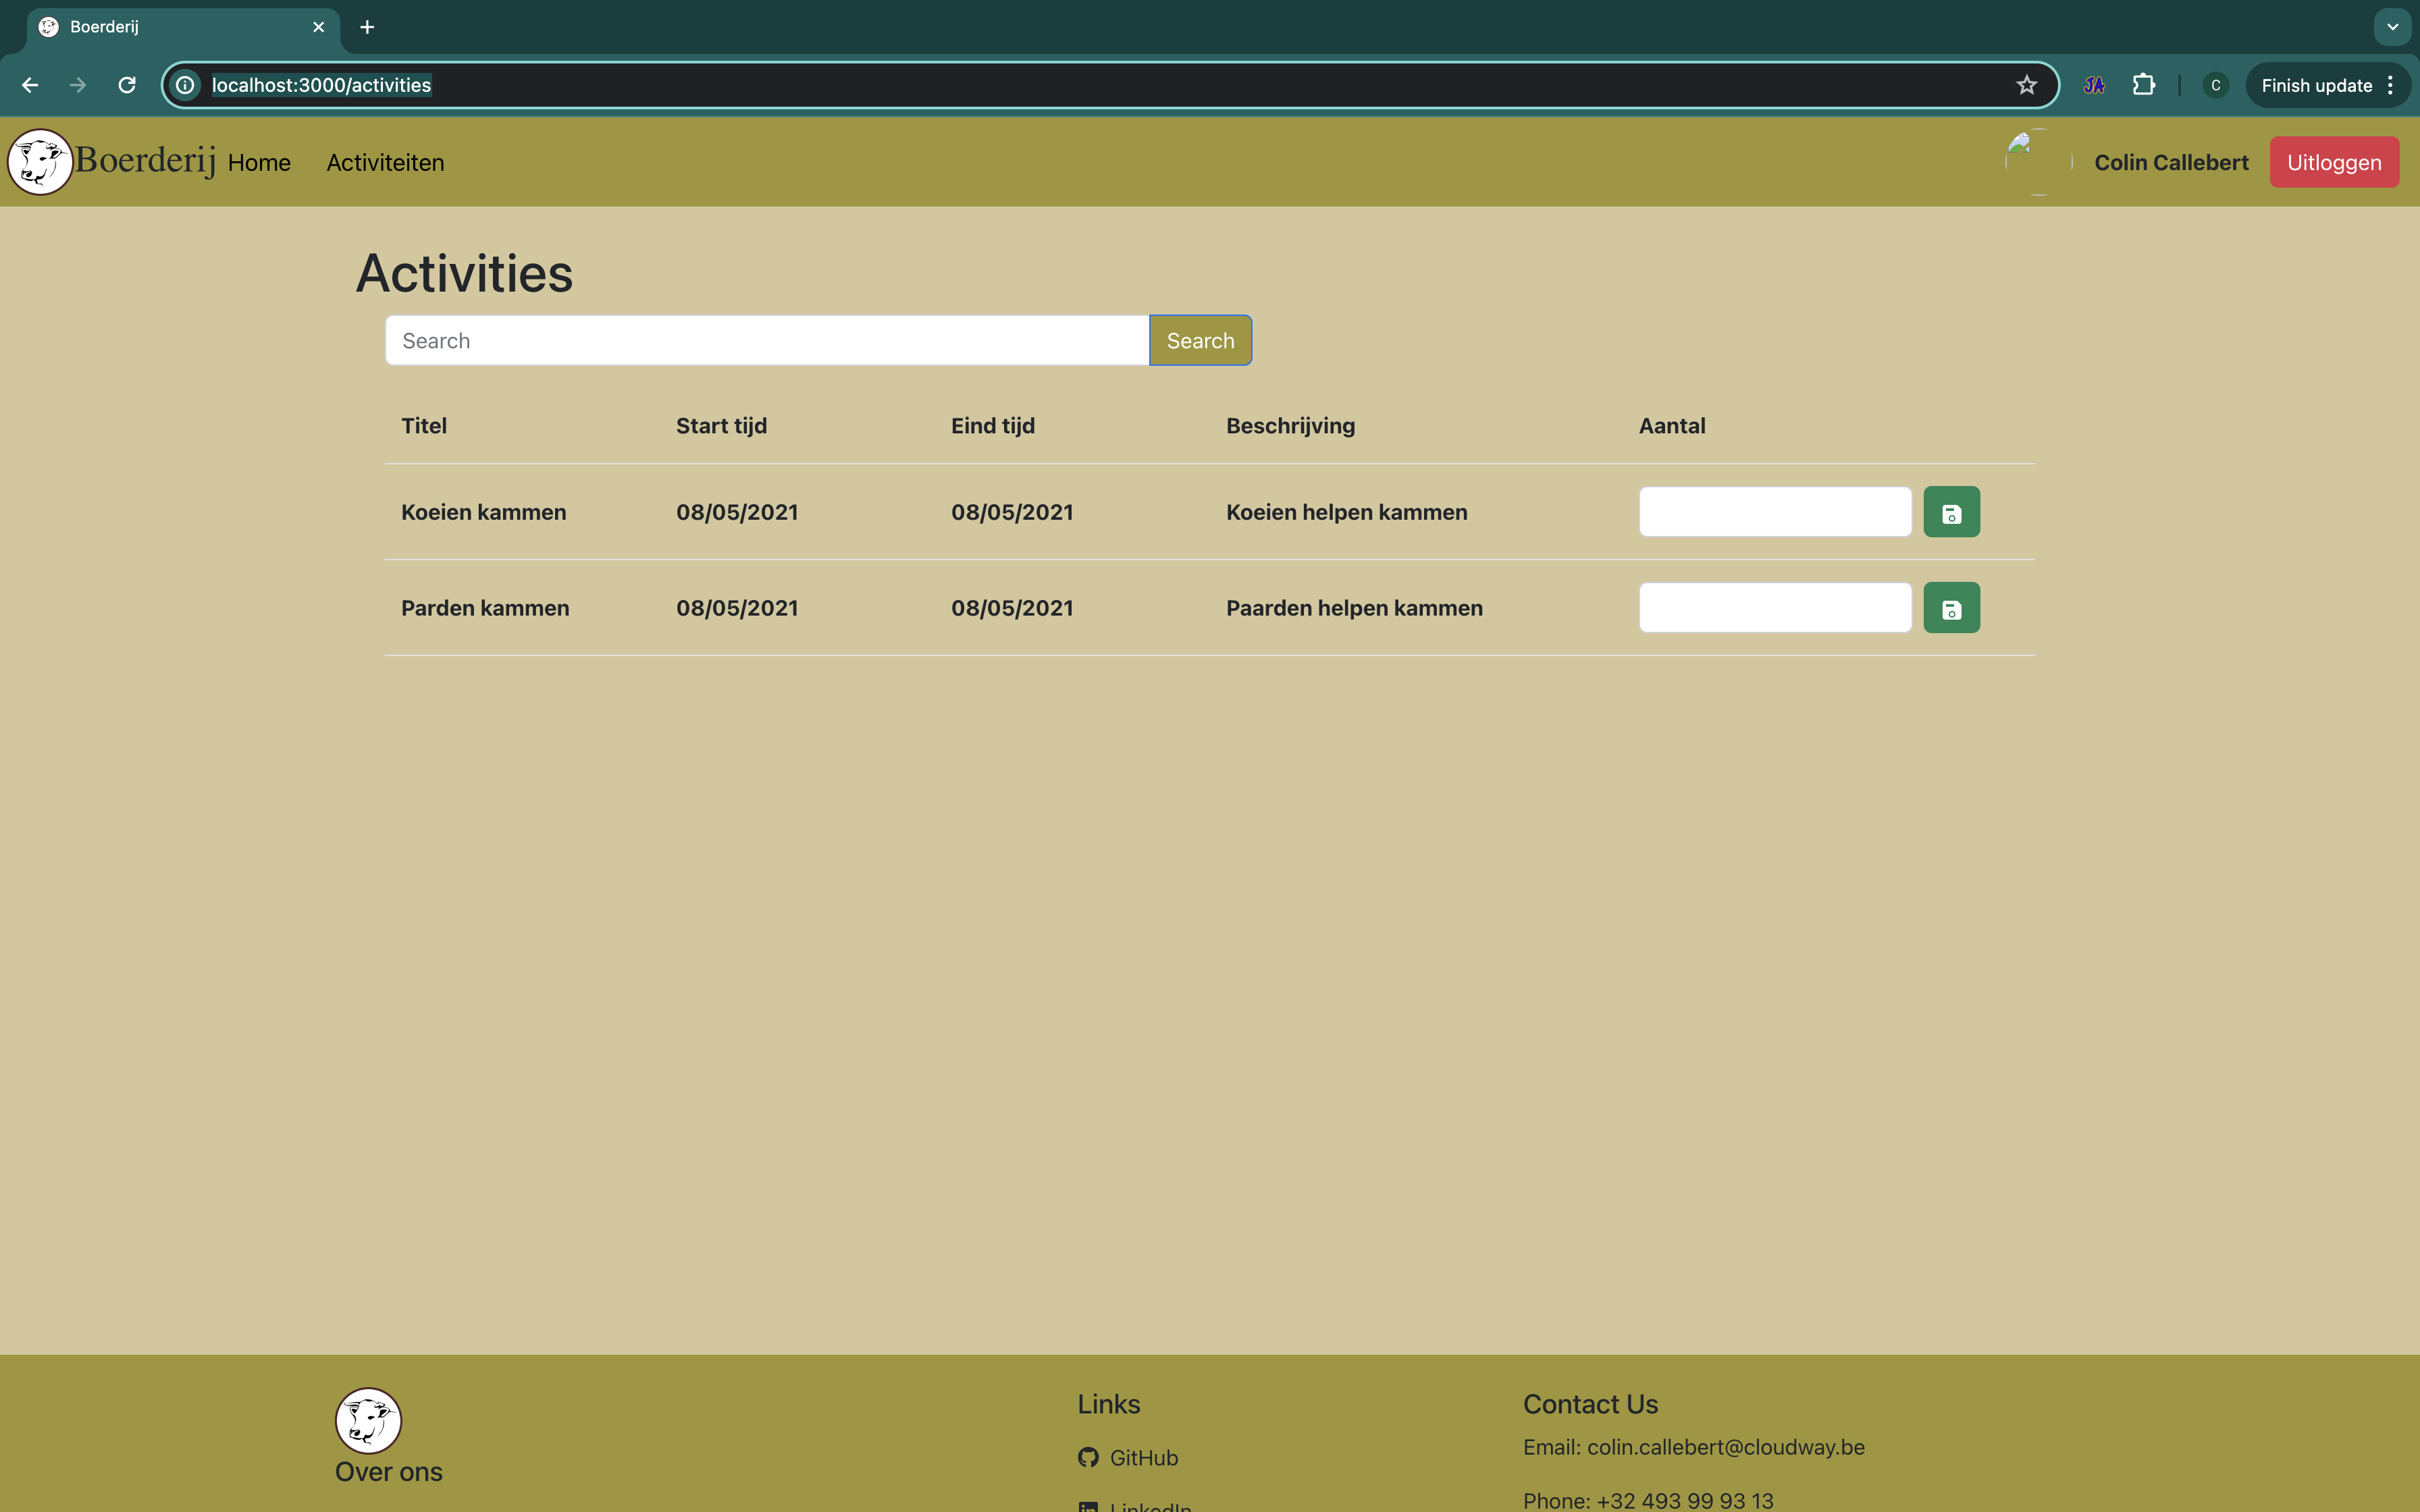
\includegraphics[width = 14cm]{Activiteiten.png} 
    \caption{Activiteitenpagina} 
    \label{fig:activities}
\end{figure}

De gebruiker kan zich inschrijven voor een activiteit door een aantal in te geven en op de knop te klikken.

\begin{figure}[H]
    \centering	
    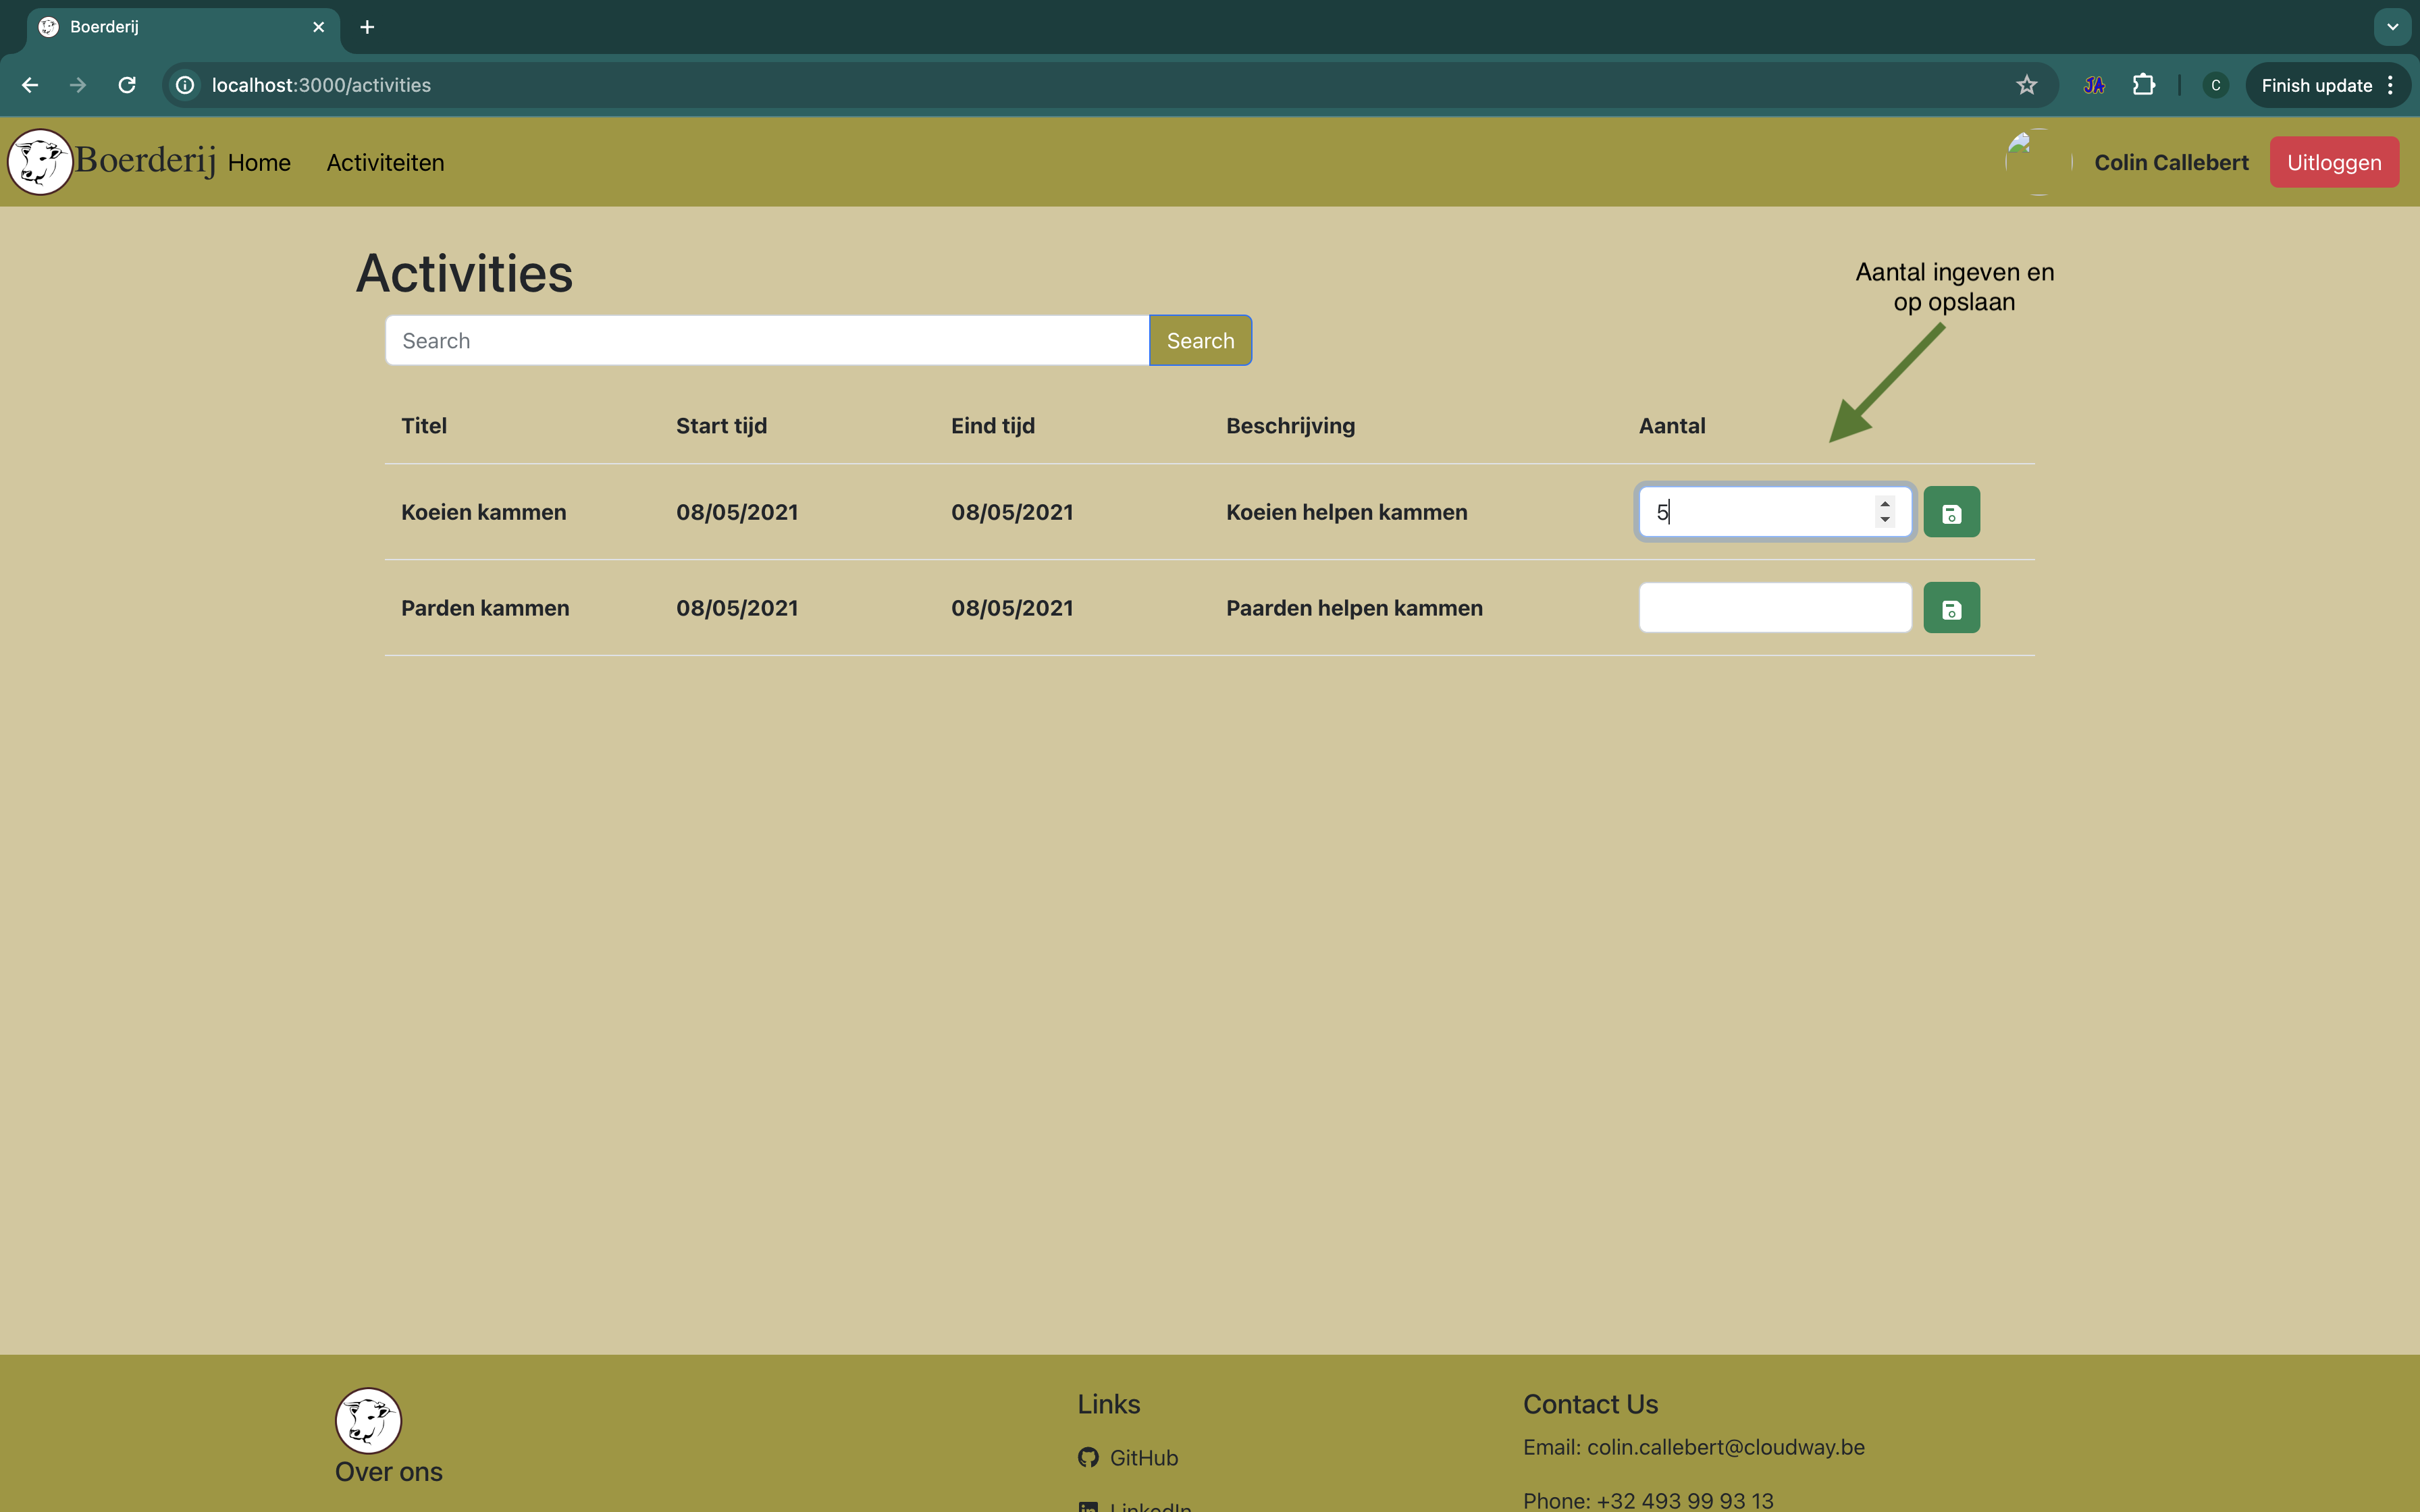
\includegraphics[width = 14cm]{ActiviteitAdd.png} 
    \caption{Inschrijven voor activiteit} 
    \label{fig:subscribe}
\end{figure}

Na het inschrijven voor een activiteit krijgt de gebruiker een bevestiging te zien.

\begin{figure}[H]
    \centering	
    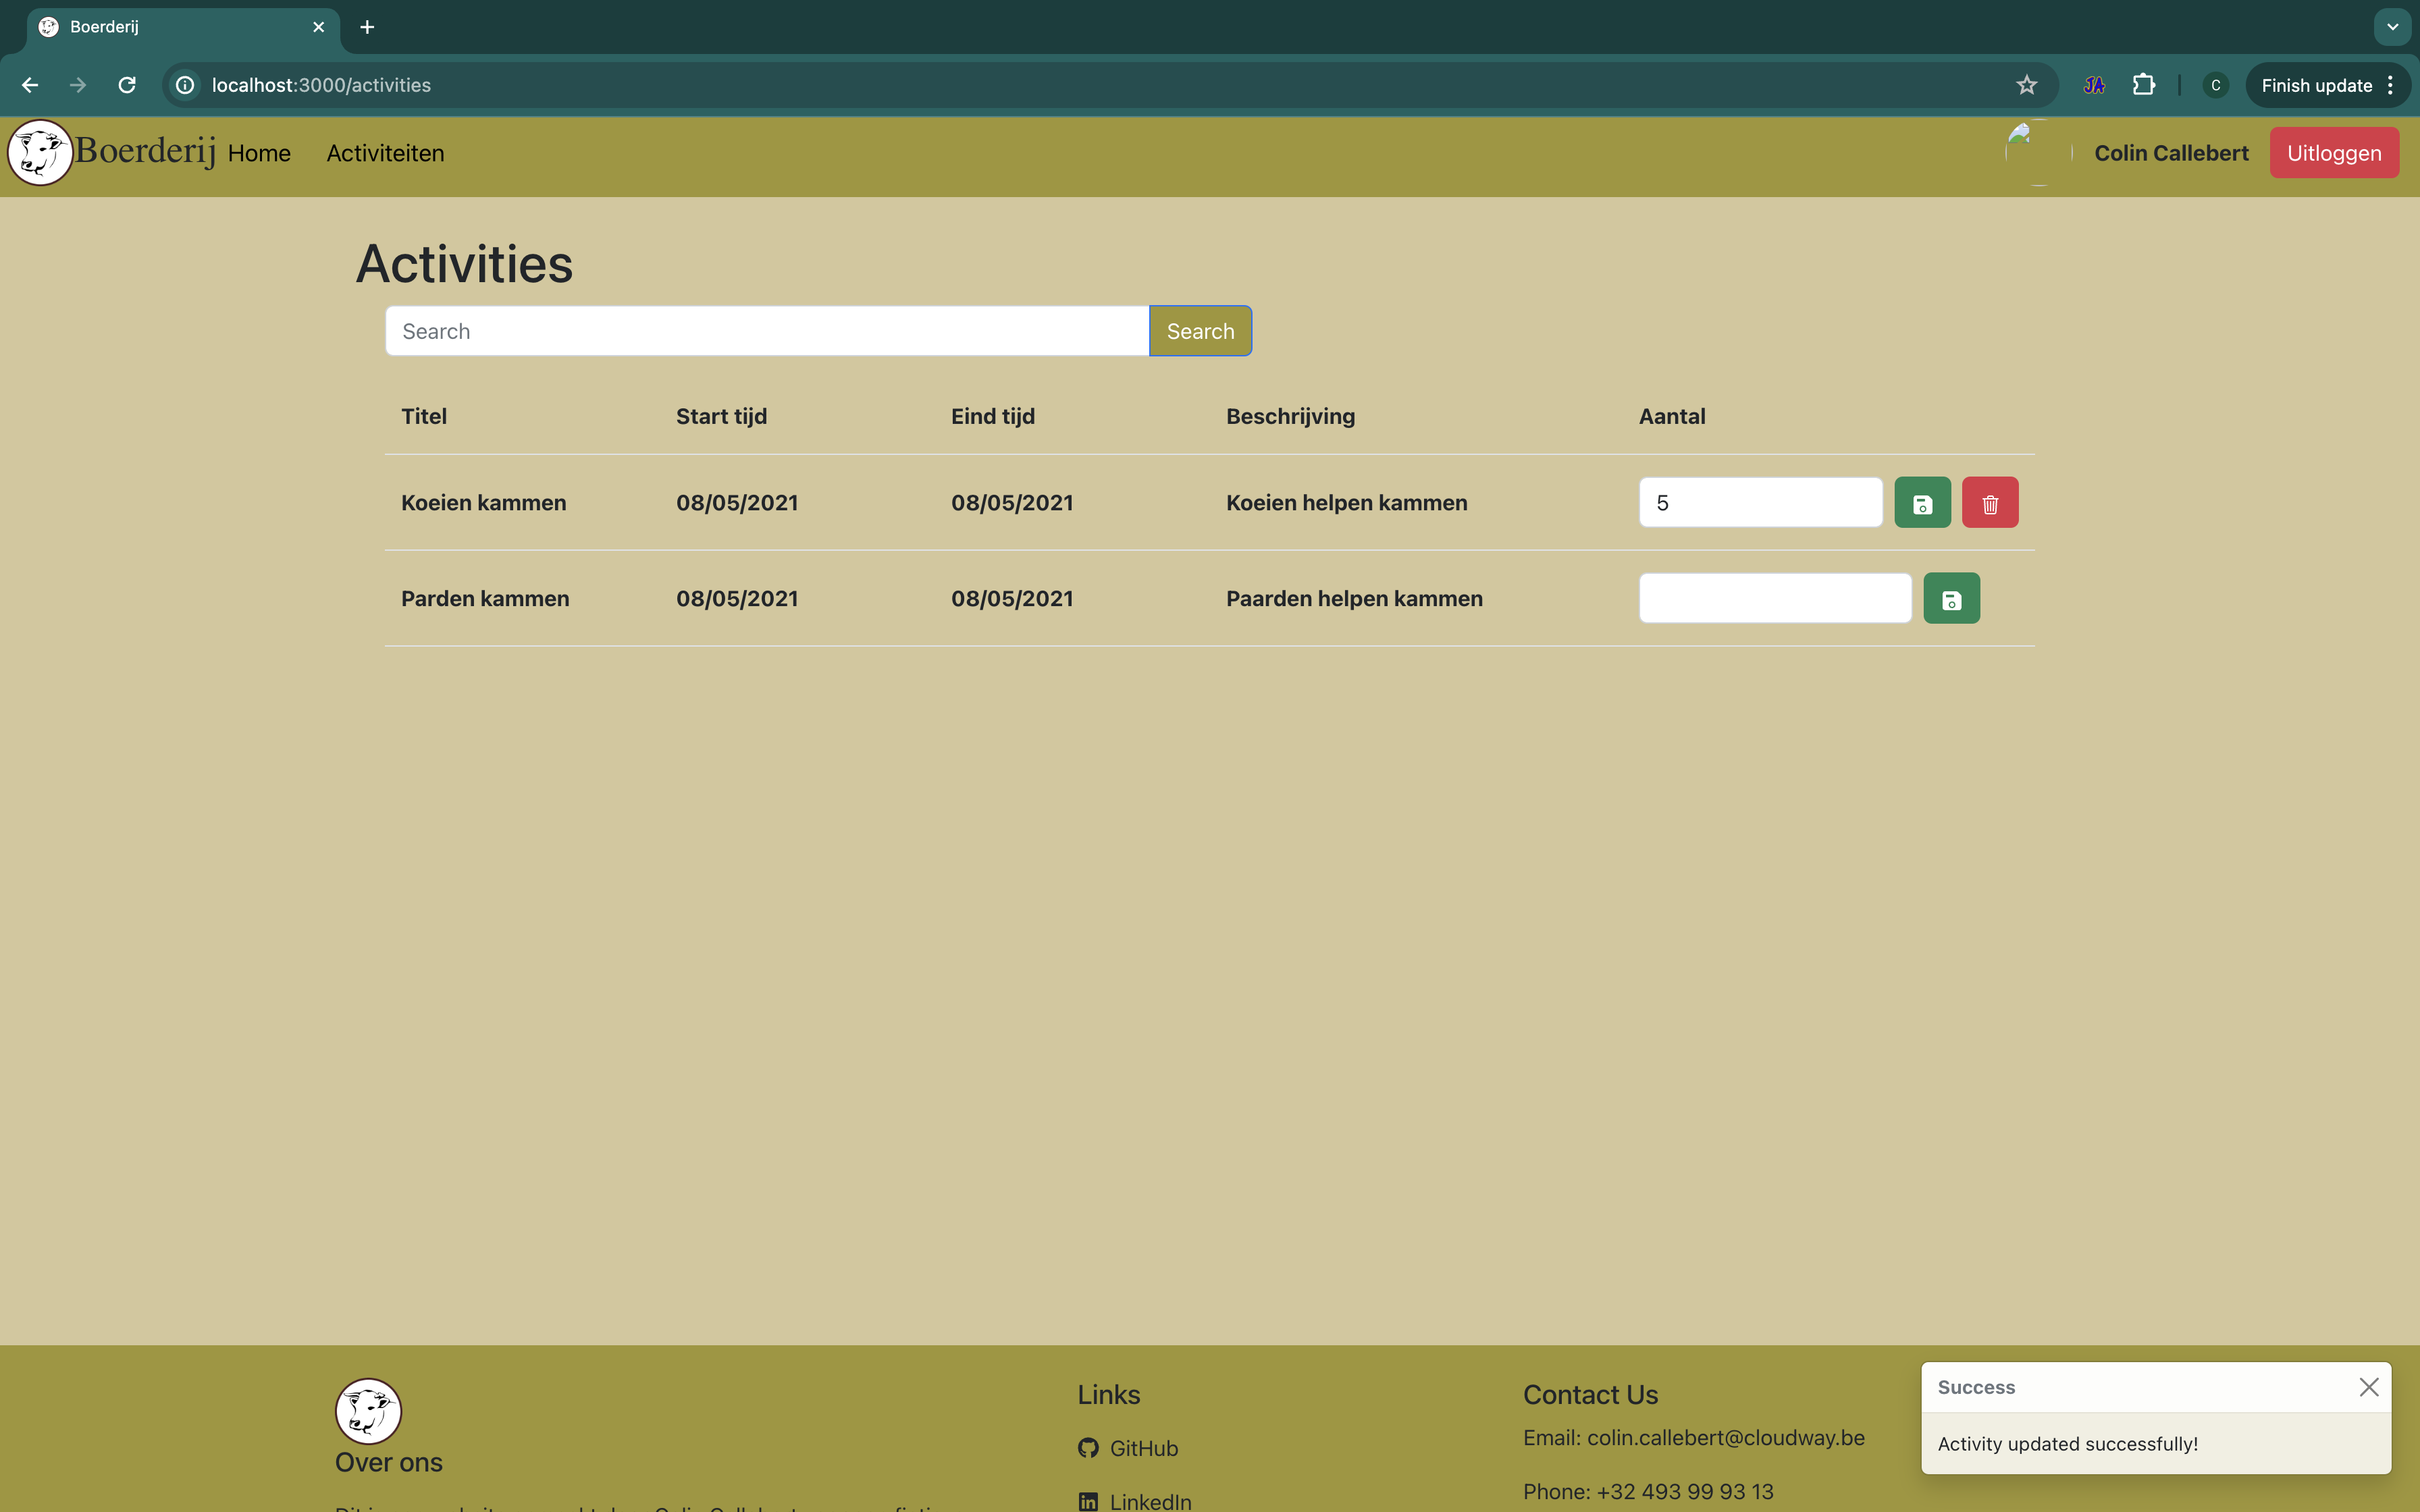
\includegraphics[width = 14cm]{ActiviteitAdd2.png} 
    \caption{Bevestiging inschrijving activiteit} 
    \label{fig:confirm}
\end{figure}

De gebruiker kan er ook voor kiezen om zich uit te schrijven voor een activiteit.

\begin{figure}[H]
    \centering	
    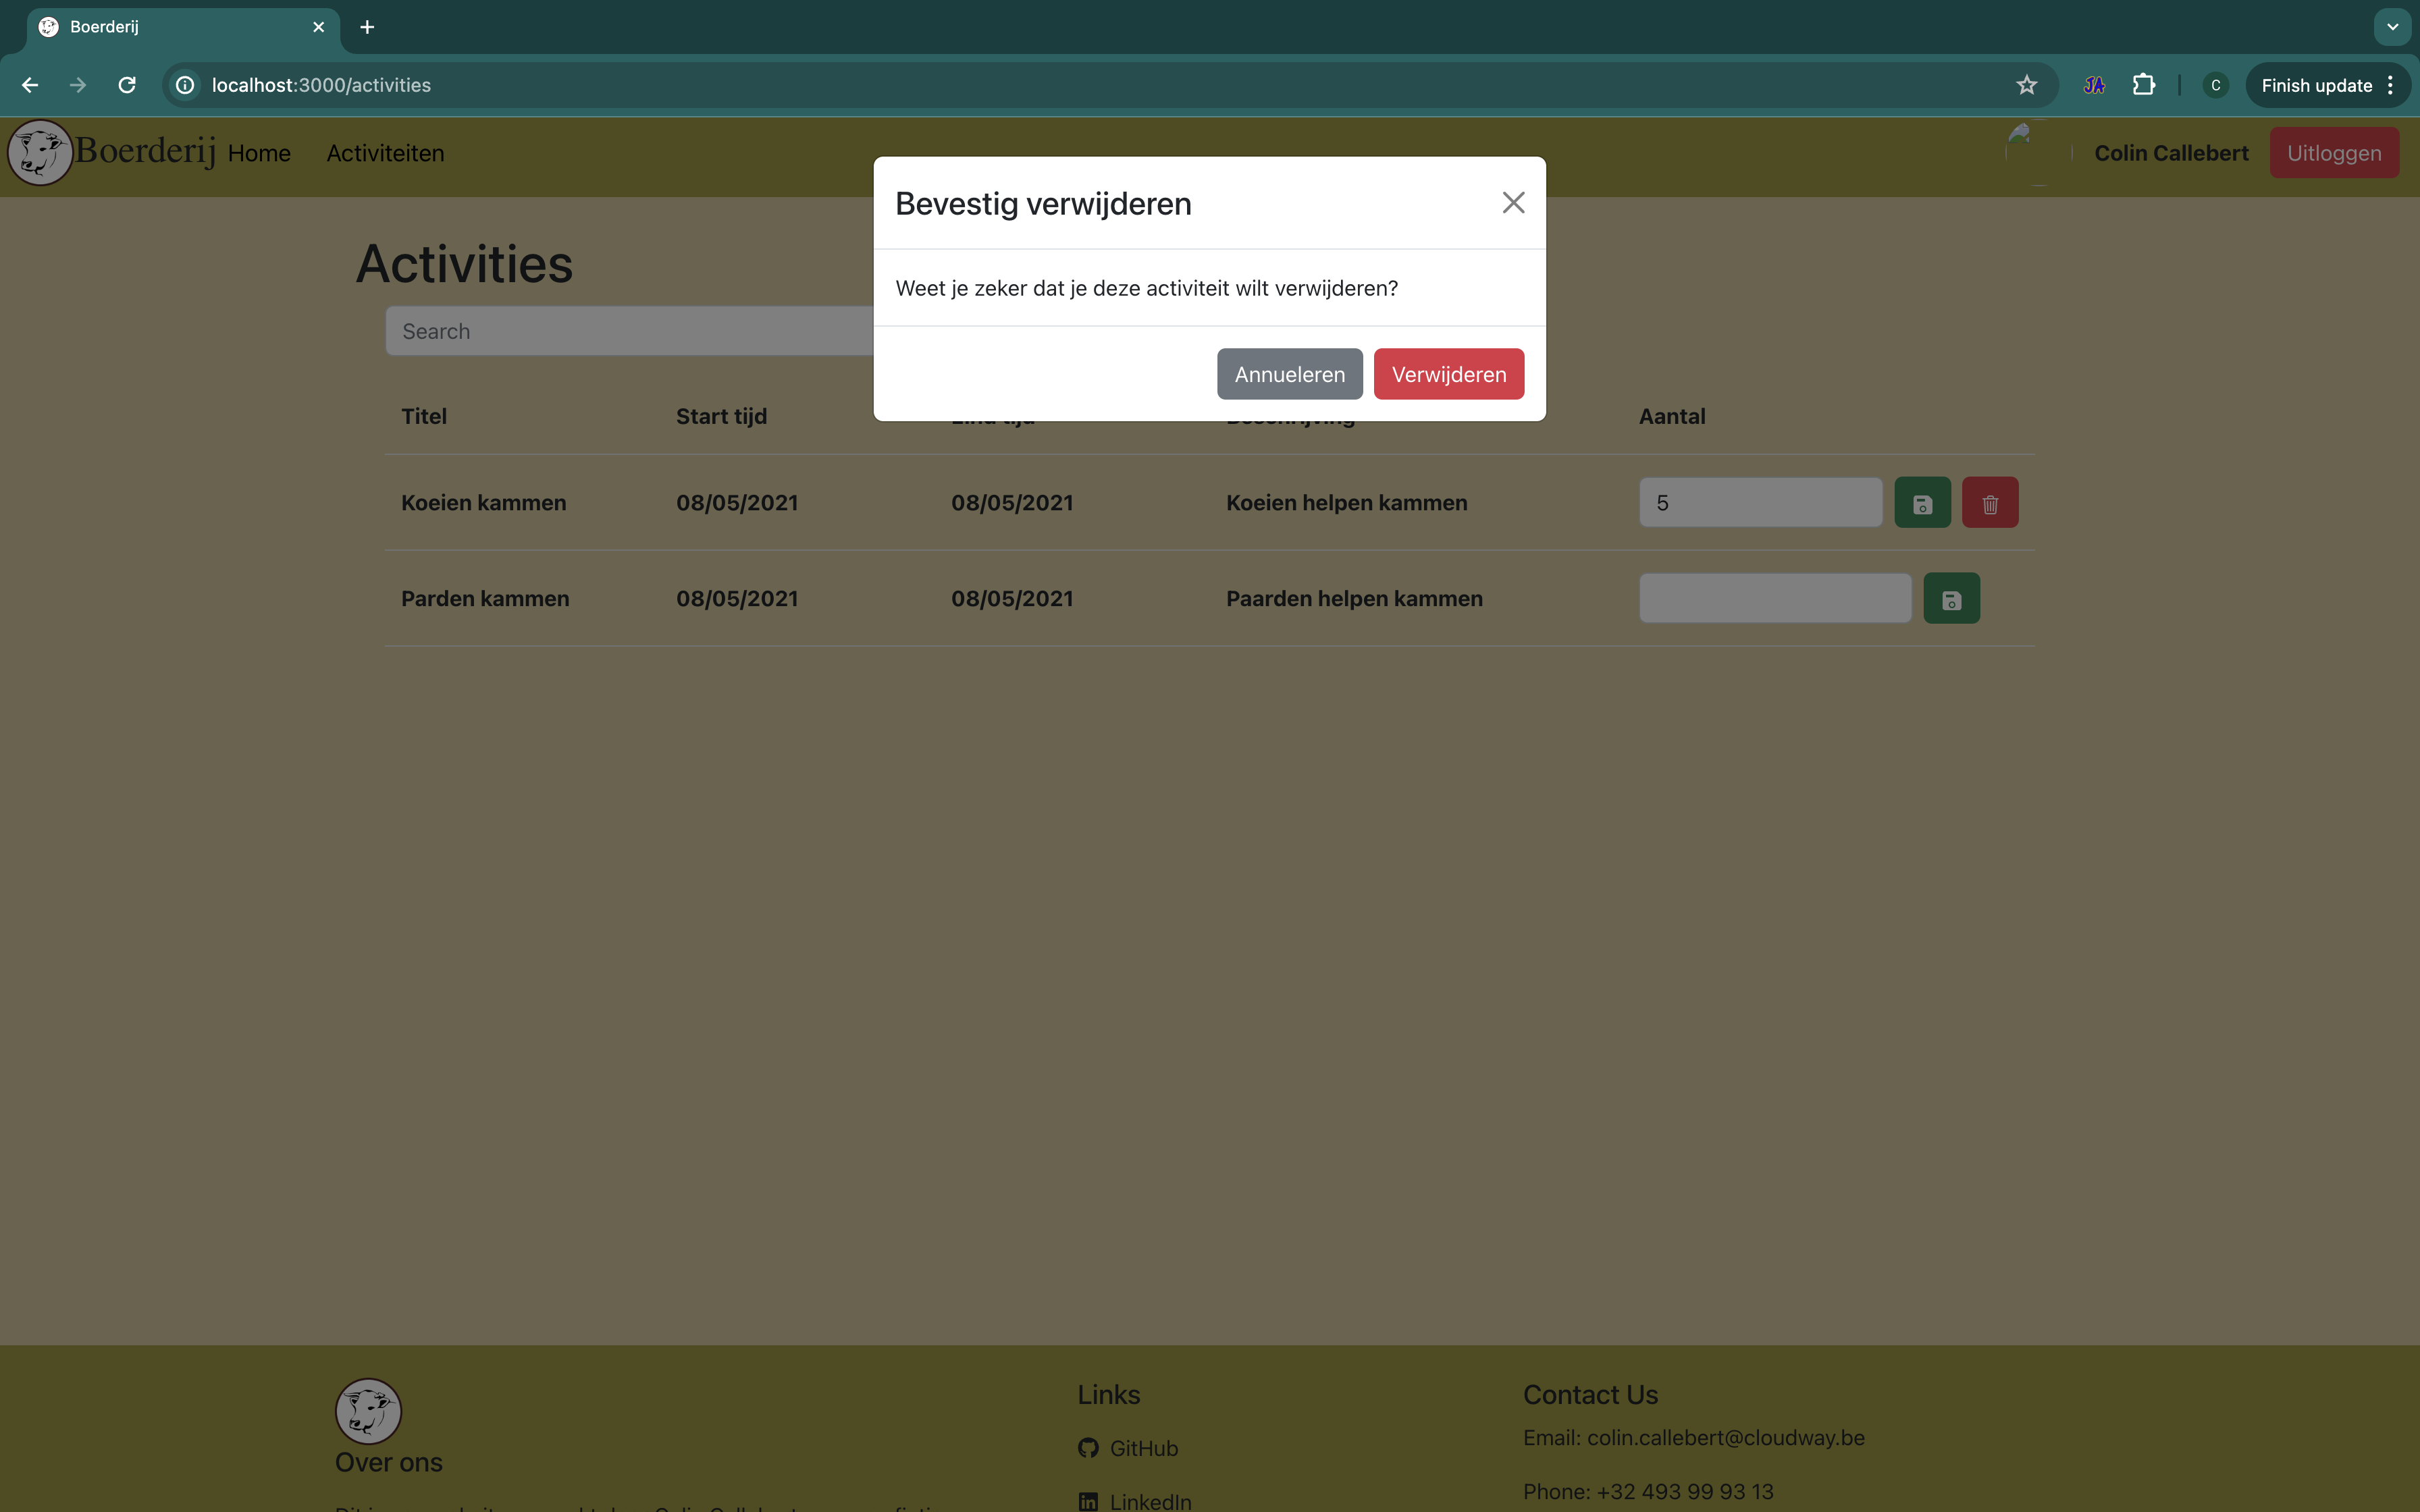
\includegraphics[width = 14cm]{ActiviteitRemove.png} 
    \caption{Uitschrijven voor activiteit} 
    \label{fig:unsubscribe}
\end{figure}

Deze versie biedt een goede basis voor de verdere ontwikkeling van de applicatie die dan opgesplitst kan worden in microservices.

Vervolgens wordt het monolithische ontwerp opgesplitst en herstructureerd naar drie afzonderlijke services, elk verantwoordelijk voor specifieke functionaliteiten. Deze aanpak stelt me in staat om de modulariteit, onderhoudbaarheid en schaalbaarheid van het systeem te verbeteren, terwijl ook de ontwikkeling en implementatie van nieuwe features wordt vergemakkelijkt.


\chapter{\IfLanguageName{dutch}{Opsplitsen en herstructureren van de backend}{Splitting up and restructuring the backend}}
\label{ch:opsplitsen-backend}

In de volgende fase van het onderzoek was het herstructureren van de backend en het opdelen in drie afzonderlijke services, de cruciale eerste stap in de omschakeling van monoliet naar services. 
\begin{figure}
	\centering	
	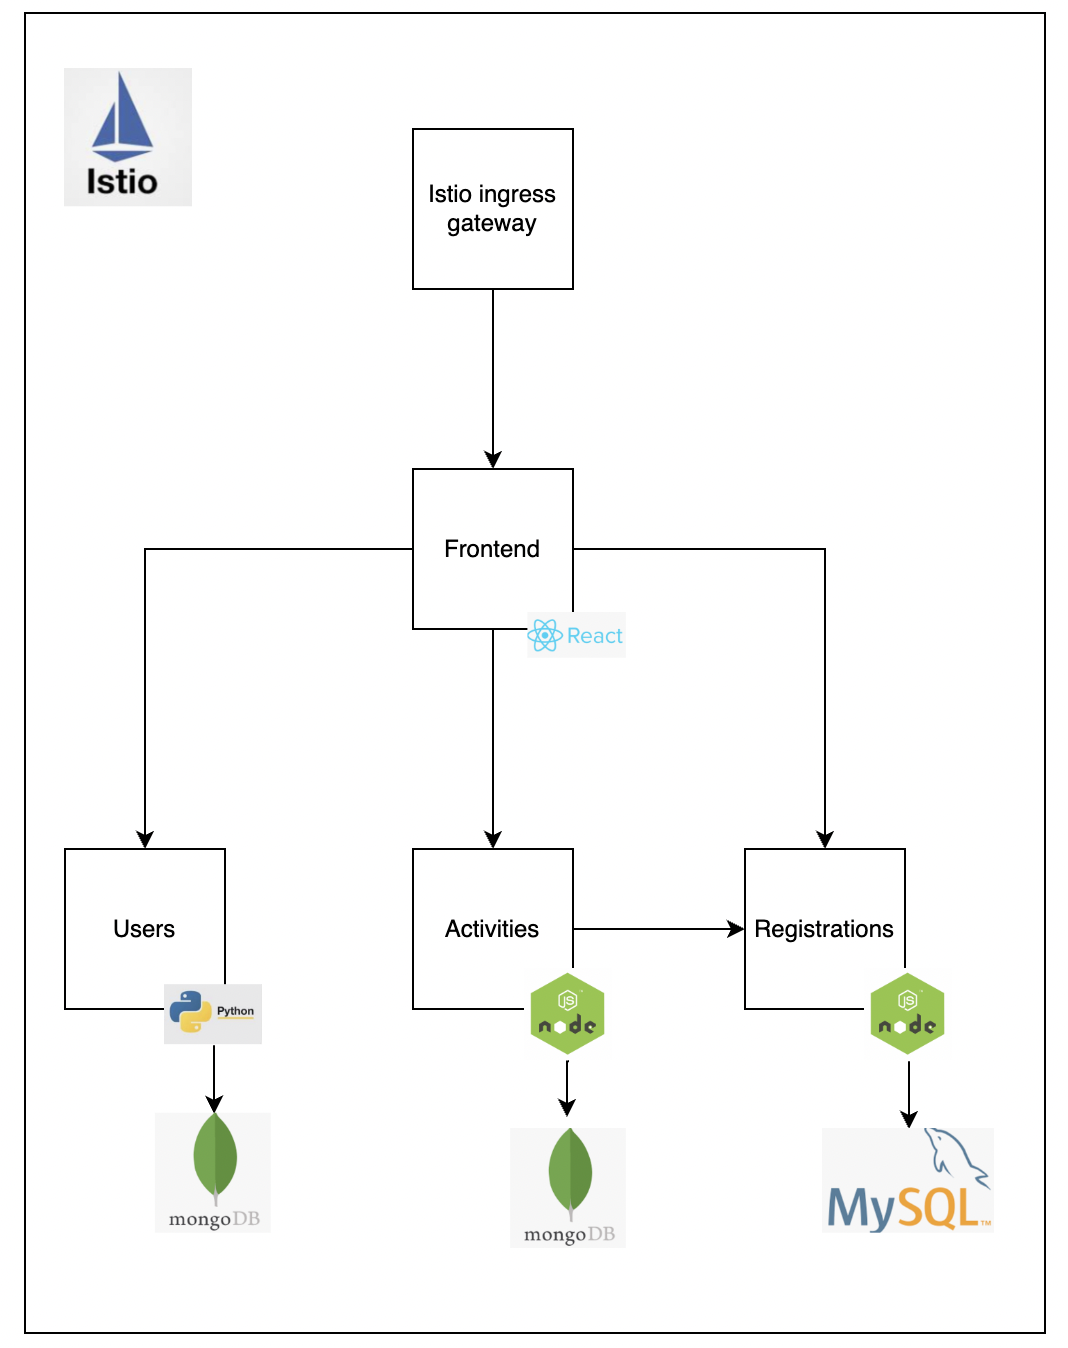
\includegraphics[width = 8cm]{services.png} 
	\caption{Architectuur services} 
	\label{fig:services} 
\end{figure}
\FloatBarrier

Er zijn drie services gedefinieerd: een gebruikersservice, een activiteitenservice en een registratieservice. Deze services zijn verantwoordelijk voor respectievelijk het beheren van gebruikersgegevens, activiteiten en registratiegegevens. Door deze services te scheiden, kan elke service onafhankelijk worden ontwikkeld, getest en geschaald.

Voor gebruikers- en activiteitengedeelte werd gekozen om gebruik te maken van een NoSQL-database, omdat deze data statisch is en niet vaak verandert. Voor het registratiegedeelte werd gekozen voor een relationele database, omdat deze data vaak verandert en er veel transacties zijn.

Allereerst werd het gebruikersgedeelte getransformeerd van Node.js naar Python, waarbij ervoor gezorgd werd dat het zijn gegevens ophaalde uit een MongoDB-database.

Het omzetten van de data van MySql naar MonogDB is gebeurd door de data te exporteren naar een JSON-bestand en vervolgens te importeren in de MongoDB-database.

Het activiteitengedeelte van de backend heb ik echter in Node.js gehouden, waarbij ervoor gezorgd is dat het ook zijn gegevens ophaalt uit de MongoDB-database.

Het registratiegedeelte van de backend blijft ook in Node.js, maar blijft gebruik maken van een MySQL-database voor gegevensopslag. Deze keuze is gebaseerd op de specifieke vereisten van het registratieproces, waarbij MySQL wordt gekozen vanwege zijn robuuste transactiemogelijkheden en uitstekende ondersteuning voor relationele gegevensmodellering. Het gebruik van een aparte databaseoplossing voor dit gedeelte van de backend stelt me in staat om optimaal te profiteren van de unieke kenmerken en voordelen van MySQL. De code moet worden aangepast omdat gebruikers en activiteiten nu aparte services zijn. Deze moeten worden aangeroepen vanuit de registratieservice. Om onafhankelijk van deze services te kunnen ontwikkelen, worden deze in eerste instantie vervangen door stubs.

Technisch gezien wordt de Python-code van de backend uitgevoerd in Unicorn, een lightweight ASGI (Asynchronous Server Gateway Interface) compatibele webserver voor Python. Een `service.py`-bestand wordt gebruikt om de service te starten en alle endpoints te definiëren. De keuze voor Unicorn als ASGI-server biedt een robuuste en betrouwbare uitvoeringsomgeving voor Python-toepassingen. Door de ondersteuning voor asynchrone verwerking van aanvragen kunnen optimale prestaties en schaalbaarheid worden gegarandeerd.

Aan de andere kant wordt het Node.js-gedeelte van de backend uitgevoerd met behulp van Express, waarbij een `express.js`-bestand wordt gebruikt om de service te starten en alle endpoints te definiëren. Express staat bekend om zijn eenvoud en flexibiliteit, waardoor het een populaire keuze is voor het ontwikkelen van webapplicaties in Node.js. Door gebruik te maken van Express kan ik snel en efficiënt RESTful API's implementeren en beheren.

Het feit dat deze services lokaal op verschillende poorten draaien, draagt bij aan de isolatie en modulariteit van het systeem, waardoor elk onderdeel onafhankelijk kan worden ontwikkeld, getest en geschaald. Deze aanpak is de eerste stap in het omzetten van de monoliet naar een microservice.

In figuur \ref{fig:getUserLocal} is te zien hoe de gebruikersgegevens worden opgehaald uit de MongoDB-database lokaal op poort 9080.

\begin{figure}
	\centering	
	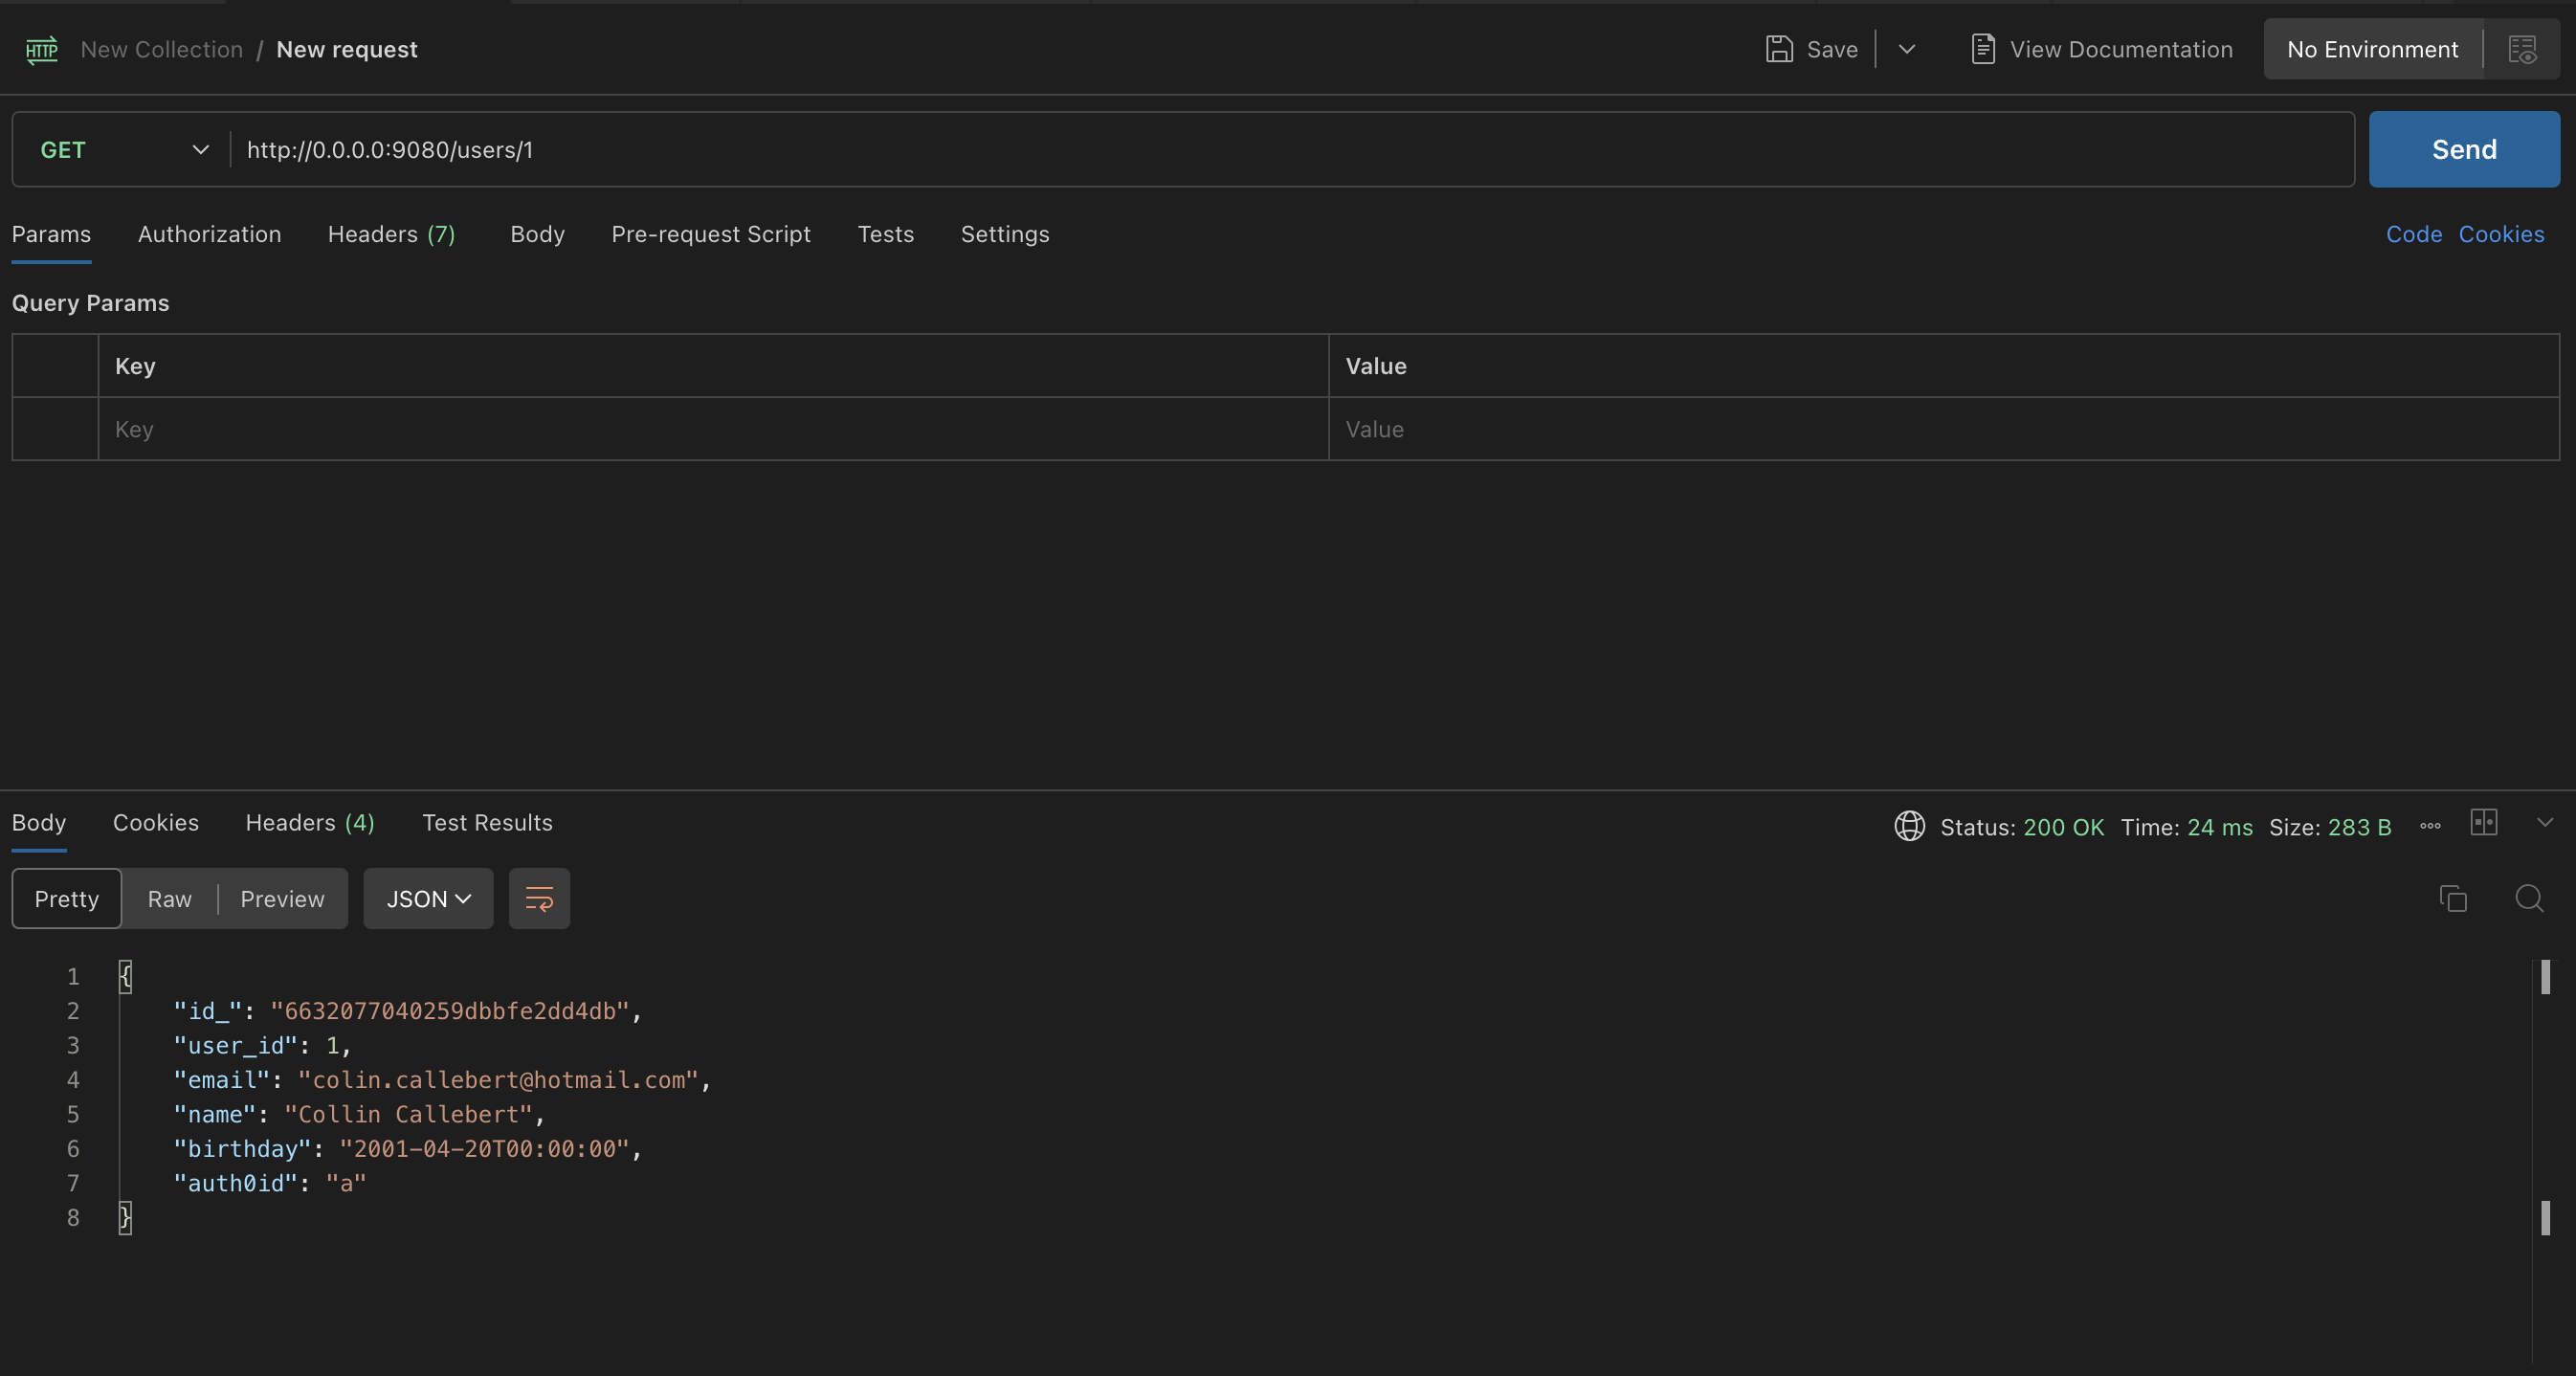
\includegraphics[width = 16cm]{getUserLocal.png} 
	\caption{Haal gebruikersgegevens op uit de MongoDB-database lokaal}
	\label{fig:getUserLocal} 
\end{figure}
\FloatBarrier
\chapter{\IfLanguageName{dutch}{Draaien backend in Docker containers}{Running backend in Docker containers}}
\label{ch:docker-backend}

Na het opsplitsen van de backend in drie afzonderlijke services, zijn ze vervolgens gecontaineriseerd door ze elk in een aparte Docker-container te plaatsen. Deze containerisatie -aanpak biedt een gestandaardiseerde en geïsoleerde omgeving voor het uitvoeren van de services.

Elke backend-service wordt nu uitgevoerd in zijn eigen Docker-container, waardoor ze volledig geïsoleerd zijn van elkaar en van andere delen van het systeem.

Voor elke service wordt een Dockerfile gemaakt om de configuratie van de respectieve containers te definiëren. Deze Dockerfiles bevatten instructies voor het bouwen van de containers, het installeren van de benodigde afhankelijkheden en het starten van de services.

Voor de Node.js code werd bijvoorbeeld een Dockerfile opgesteld die begint met het gebruik van de officiële Node.js 20-image als basis. Vervolgens worden de benodigde bestanden gekopieerd naar de werkomgeving binnen de container, dependencies geïnstalleerd met npm en de applicatie gestart met het juiste commando.

Voor de Python code werd een vergelijkbare Dockerfile gemaakt, die begint met het gebruik van de officiële Python 3.12-image als basis. Vervolgens worden de benodigde bestanden gekopieerd, dependencies geïnstalleerd met pip en de applicatie gestart met het juiste commando.

Met deze Dockerfiles kunnen de backend-services eenvoudig worden gebouwd en gedistribueerd als Docker-containers, waardoor een consistente en gecontroleerde uitvoeringsomgeving wordt gegarandeerd, ongeacht het onderliggende hostsysteem. Dit draagt bij aan een naadloze implementatie en schaalbaarheid van de applicatie in diverse omgevingen.

Met het \texttt{docker run -dp 127.0.0.1:****:9080} commando kan de container worden gestart en kan de service worden benaderd via de opgegeven poort. Op deze manier kunnen de services lokaal worden uitgevoerd en getest, voordat ze worden geïntegreerd in de bredere applicatie-architectuur.

In figuur \ref{fig:getUserDocker} is te zien hoe de gebruikersgegevens worden opgehaald uit de MongoDB-database in een Docker-container op poort ****.

\begin{figure}[H]
	\centering	
	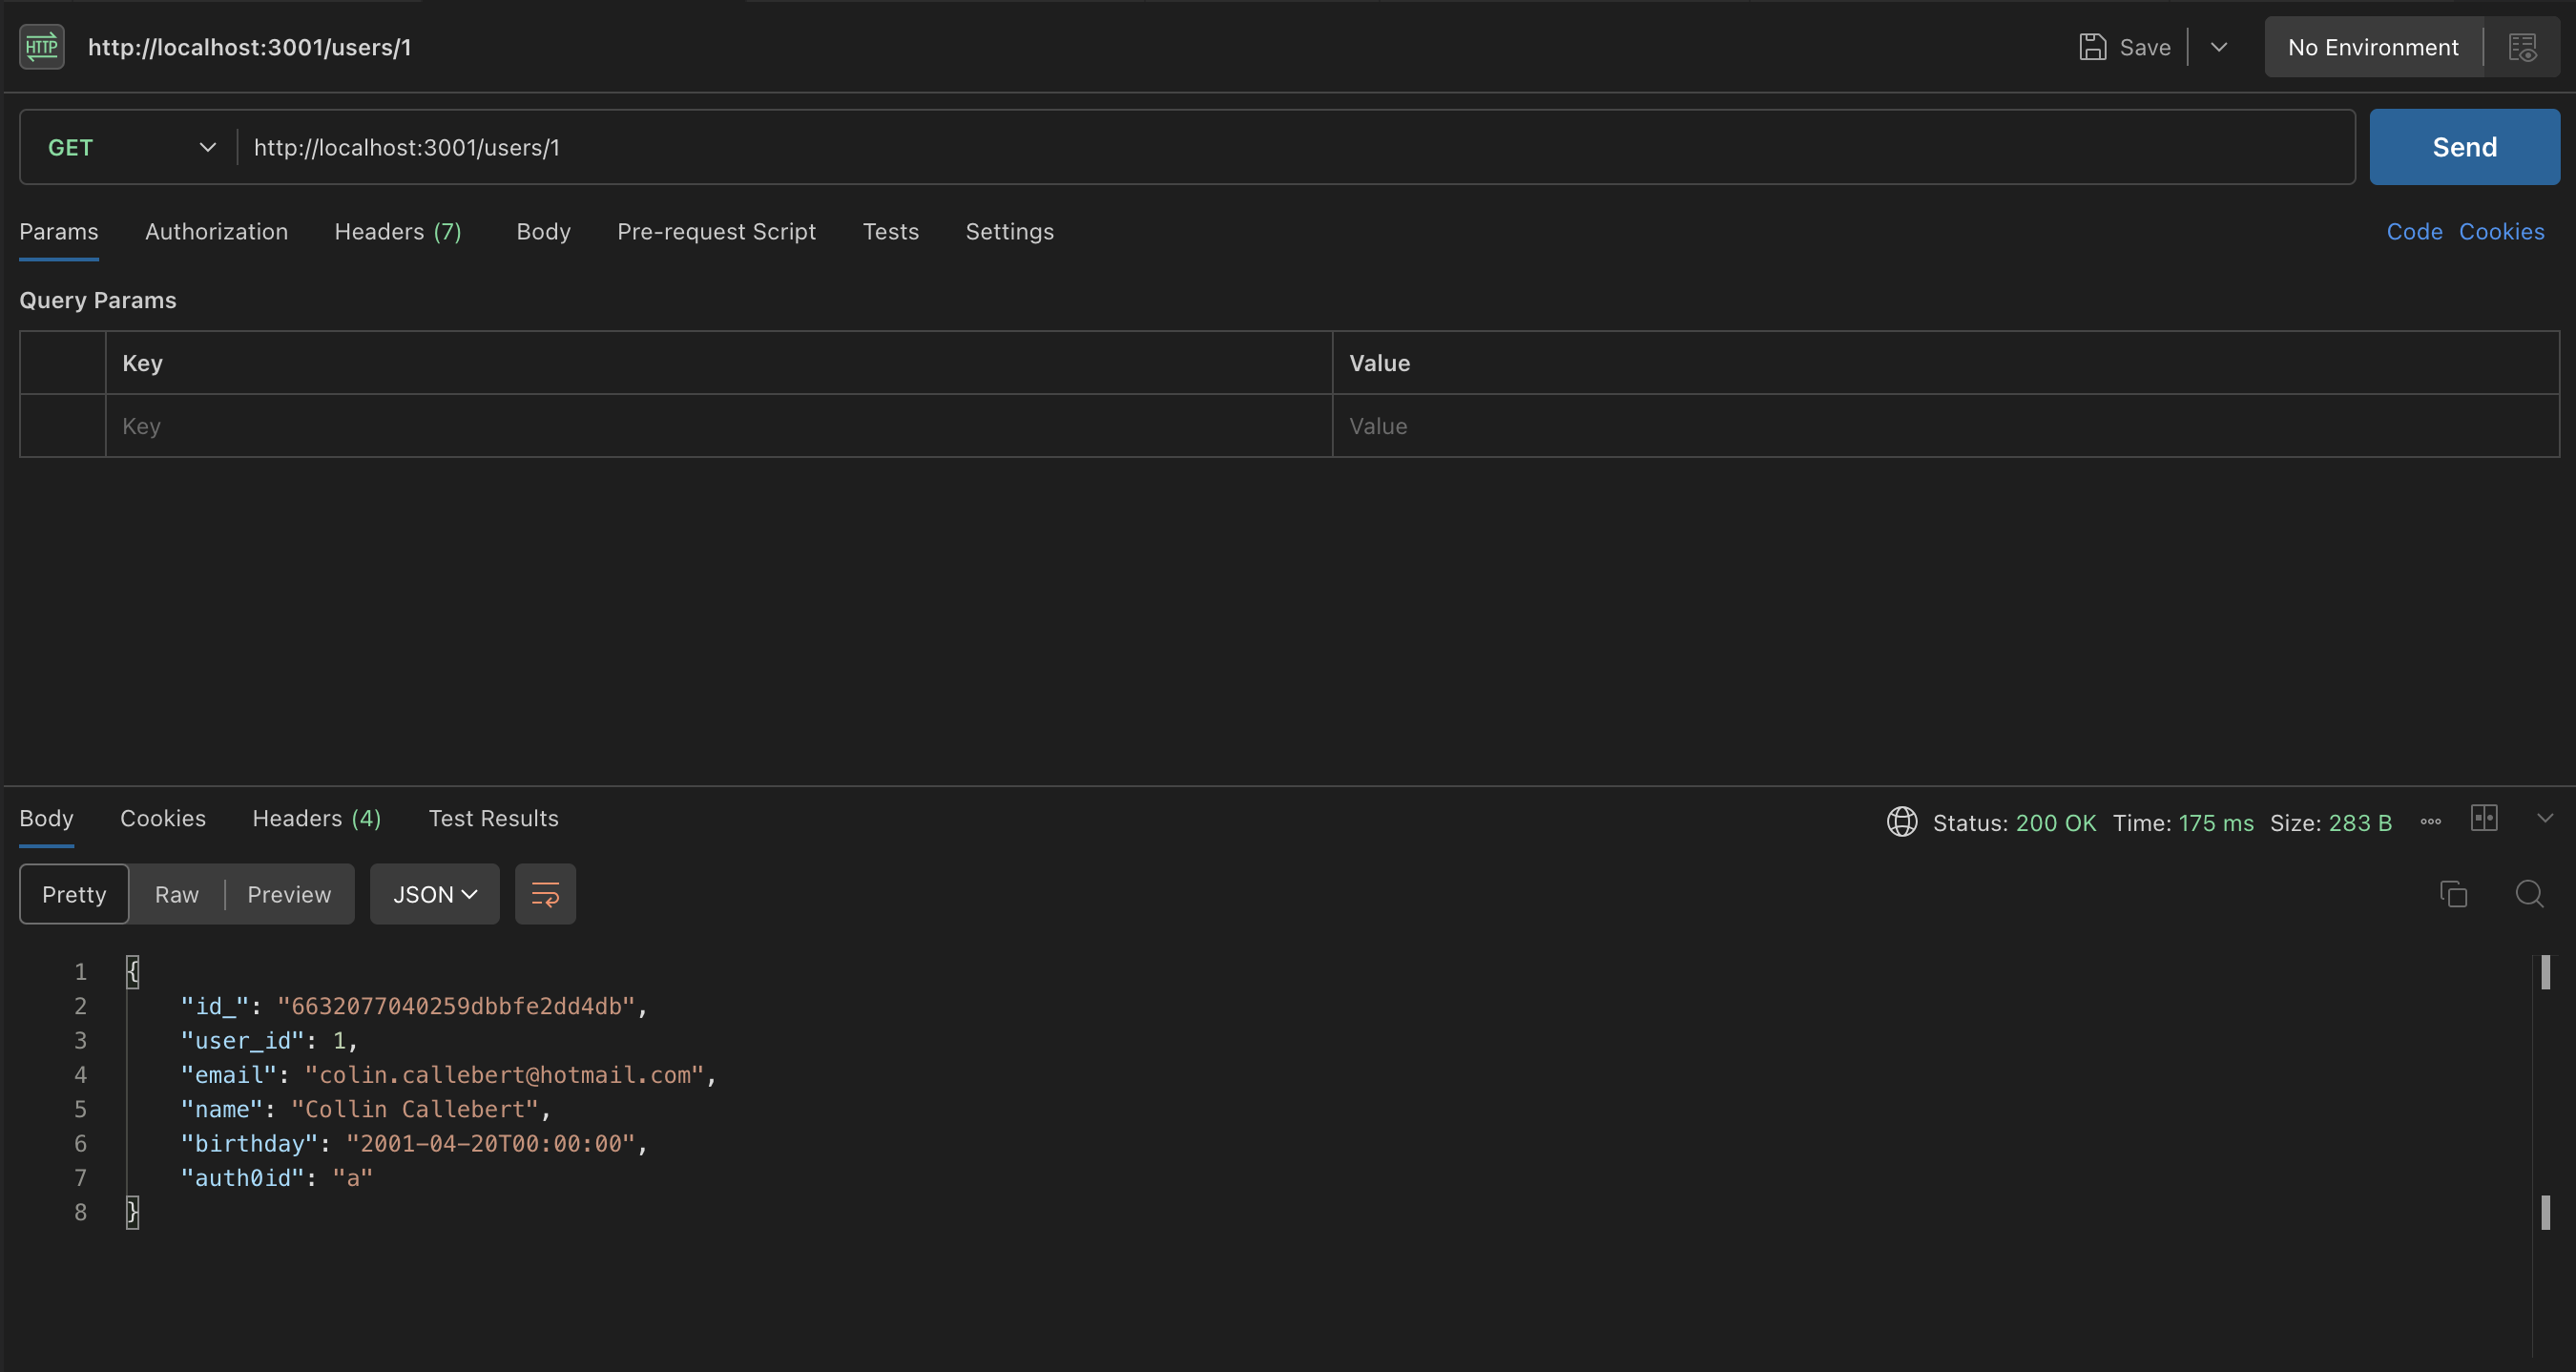
\includegraphics[width = 16cm]{getUseDocker.png} 
	\caption{Haal gebruikersgegevens op uit de MongoDB- database in een Docker-container}
	\label{fig:getUserDocker} 
\end{figure}
\FloatBarrier
\chapter{\IfLanguageName{dutch}{Implementatie in Istio}{Implementation in Istio}}
\label{ch:implementatie-backend-istio}

Om de services in Istio te implementeren, moeten we eerst de services definiëren in \textit{YAML}-bestanden. In deze bestanden definiëren we de services, de \textit{VirtualService} en de \textit{Gateway}.

De \textit{Gateway} wordt eenmalig gedefinieerd en definieert de host en de poort waarop de services van buitenaf kunnen worden benaderd. De \textit{VirtualService} definieert de regels voor het routeren van verzoeken naar de services.

Het \textit{Gateway}-bestand zorgt voor het aanmaken van de ingressgateway \ref{fig:gateway}.

De toegestane routeringen worden gedefinieerd in het \textit{VirtualService}-bestand \ref{fig:virtualservice}.

\begin{figure}[H]
    \centering	
    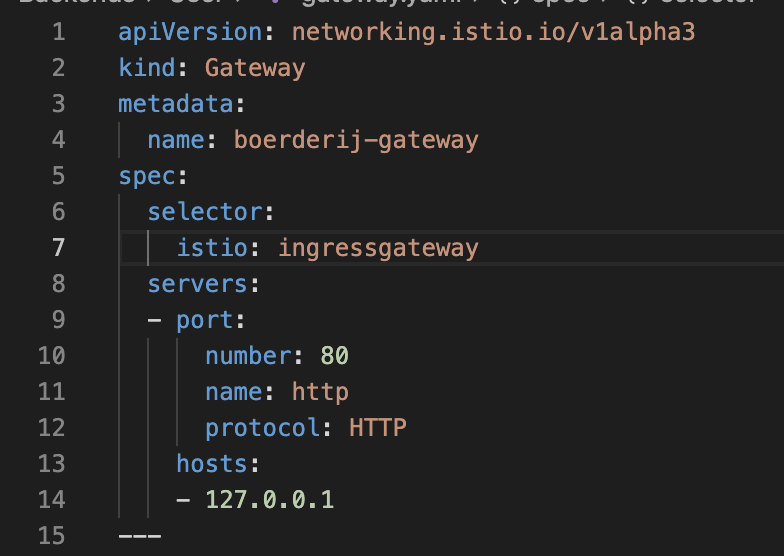
\includegraphics[width = 8cm]{gateway.png} 
    \caption{Voorbeeld van een gateway.yaml bestand} 
    \label{fig:gateway}
\end{figure}

\begin{figure}[H]
    \centering	
    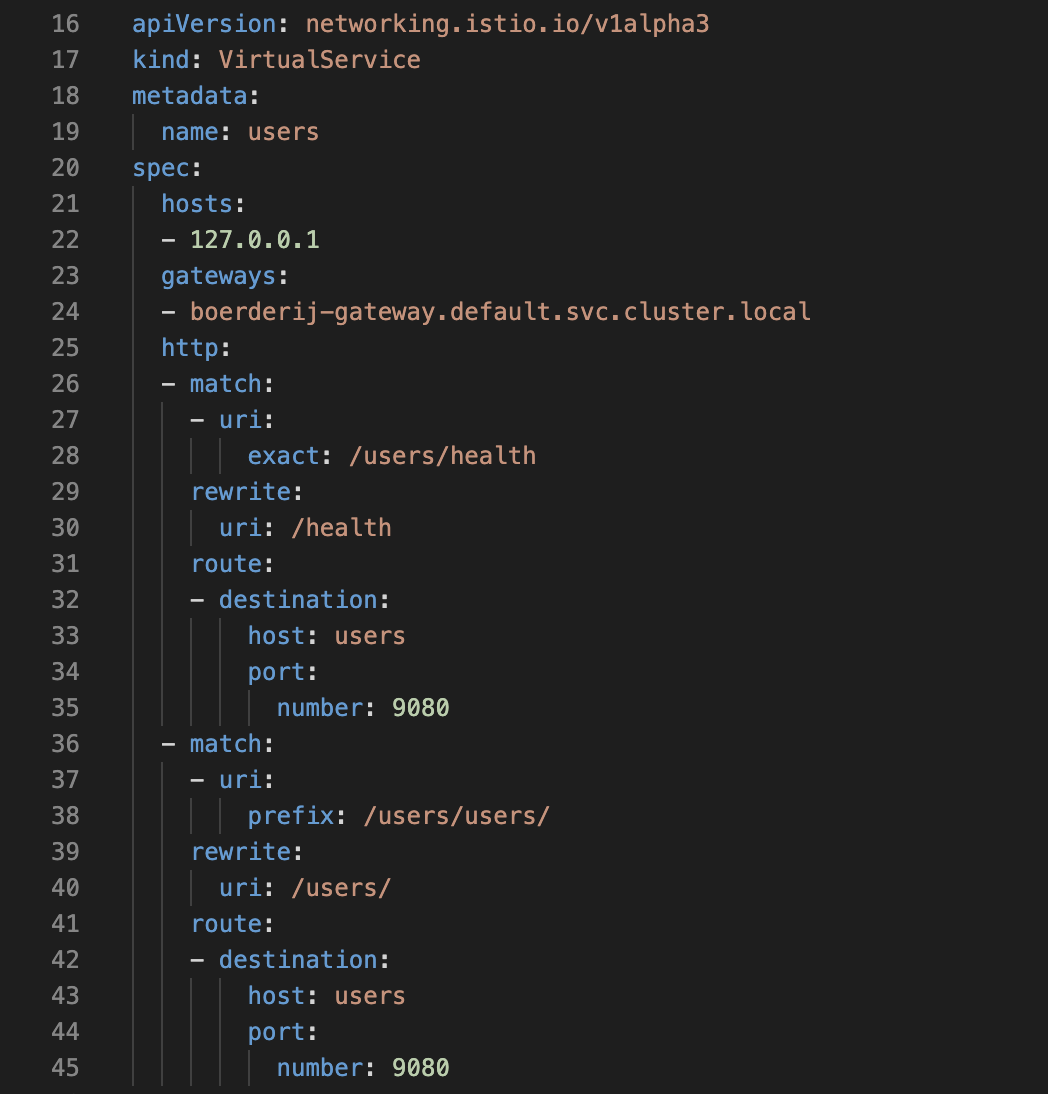
\includegraphics[width = 8cm]{virtualservice.png} 
    \caption{Voorbeeld van een virtualservice.yaml bestand} 
    \label{fig:virtualservice}
\end{figure}

De services blijven draaien in Docker-containers. De containers worden gebouwd met behulp van de Dockerfiles die in de vorige hoofdstukken zijn gemaakt. De containers worden vervolgens gedistribueerd naar een Kubernetes-cluster.

Voor het deployen van de services in Kubernetes, maken we gebruik van \textit{DeploymentYAML}-bestanden. In deze bestanden definiëren we de services, de \textit{Deployment} en de \textit{Service}. De \textit{Deployment} definieert de configuratie van de pod en de \textit{Service} definieert de configuratie van de service.

Binnen Istio krijgt elke service pod naast de applicatie container ook een \textit{sidecar} container. Deze \textit{sidecar} container is verantwoordelijk voor het routeren van het netwerkverkeer naar de applicatie container. De \textit{sidecar} container wordt automatisch toegevoegd door Istio.

Een voorbeeld van een \textit{DeploymentYAML}-bestand is te zien in figuur \ref{fig:deployment}.

\begin{figure}[H]
    \centering	
    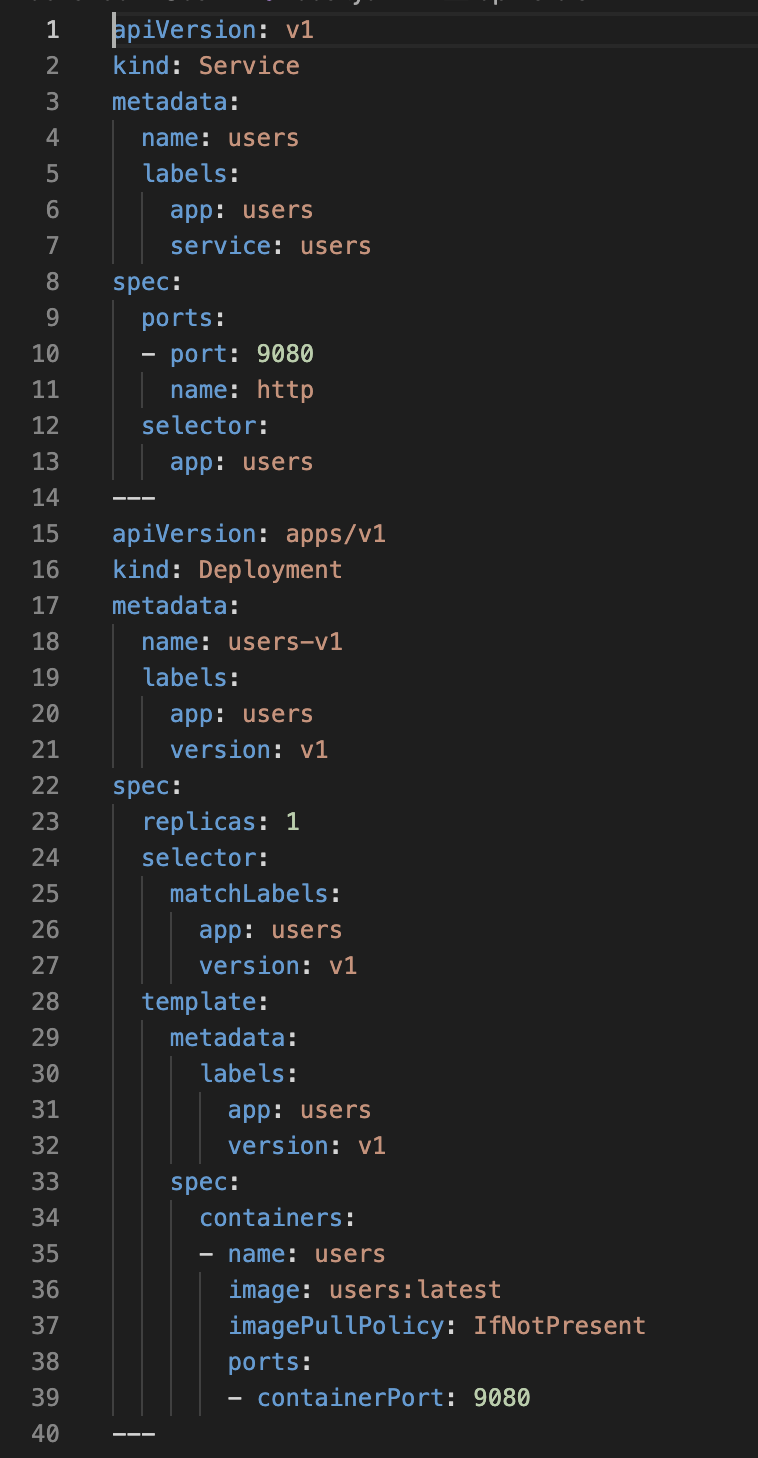
\includegraphics[width = 8cm]{deployment.png} 
    \caption{Voorbeeld van een deployment.yaml bestand} 
    \label{fig:deployment}
\end{figure}

De Kubernetes cluster draait binnen een Minikube Docker container. Om deze lokaal beschikbaar te maken, moet de Minikube tunnel worden gestart. De Minikube tunnel zorgt ervoor dat de services van buitenaf kunnen worden benaderd.

Zodra de services zijn geïmplementeerd in Istio, kunnen we de applicatie benaderen via de gateway-URL. De gateway-URL is de host en poort die is gedefinieerd in het \textit{Gateway}-bestand. De gateway-URL kan worden verkregen door de omgevingsvariabelen \textit{INGRESS\_HOST} en \textit{INGRESS\_PORT} in te stellen. Met behulp van deze omgevingsvariabelen kunnen we de gateway-URL berekenen en de applicatie benaderen via de browser.

Het Kiali-dashboard kan worden geopend met het \textit{istioctl dashboard kiali} commando. Het Kiali-dashboard geeft een visuele weergave van de interacties tussen de verschillende services. Hiermee kunnen we de verkeersstromen en de prestaties van de services monitoren en analyseren.

Wanneer er geen verkeer is, ziet het Kiali-dashboard eruit zoals in figuur \ref{fig:kaili}.
\begin{figure}[H]
    \centering	
    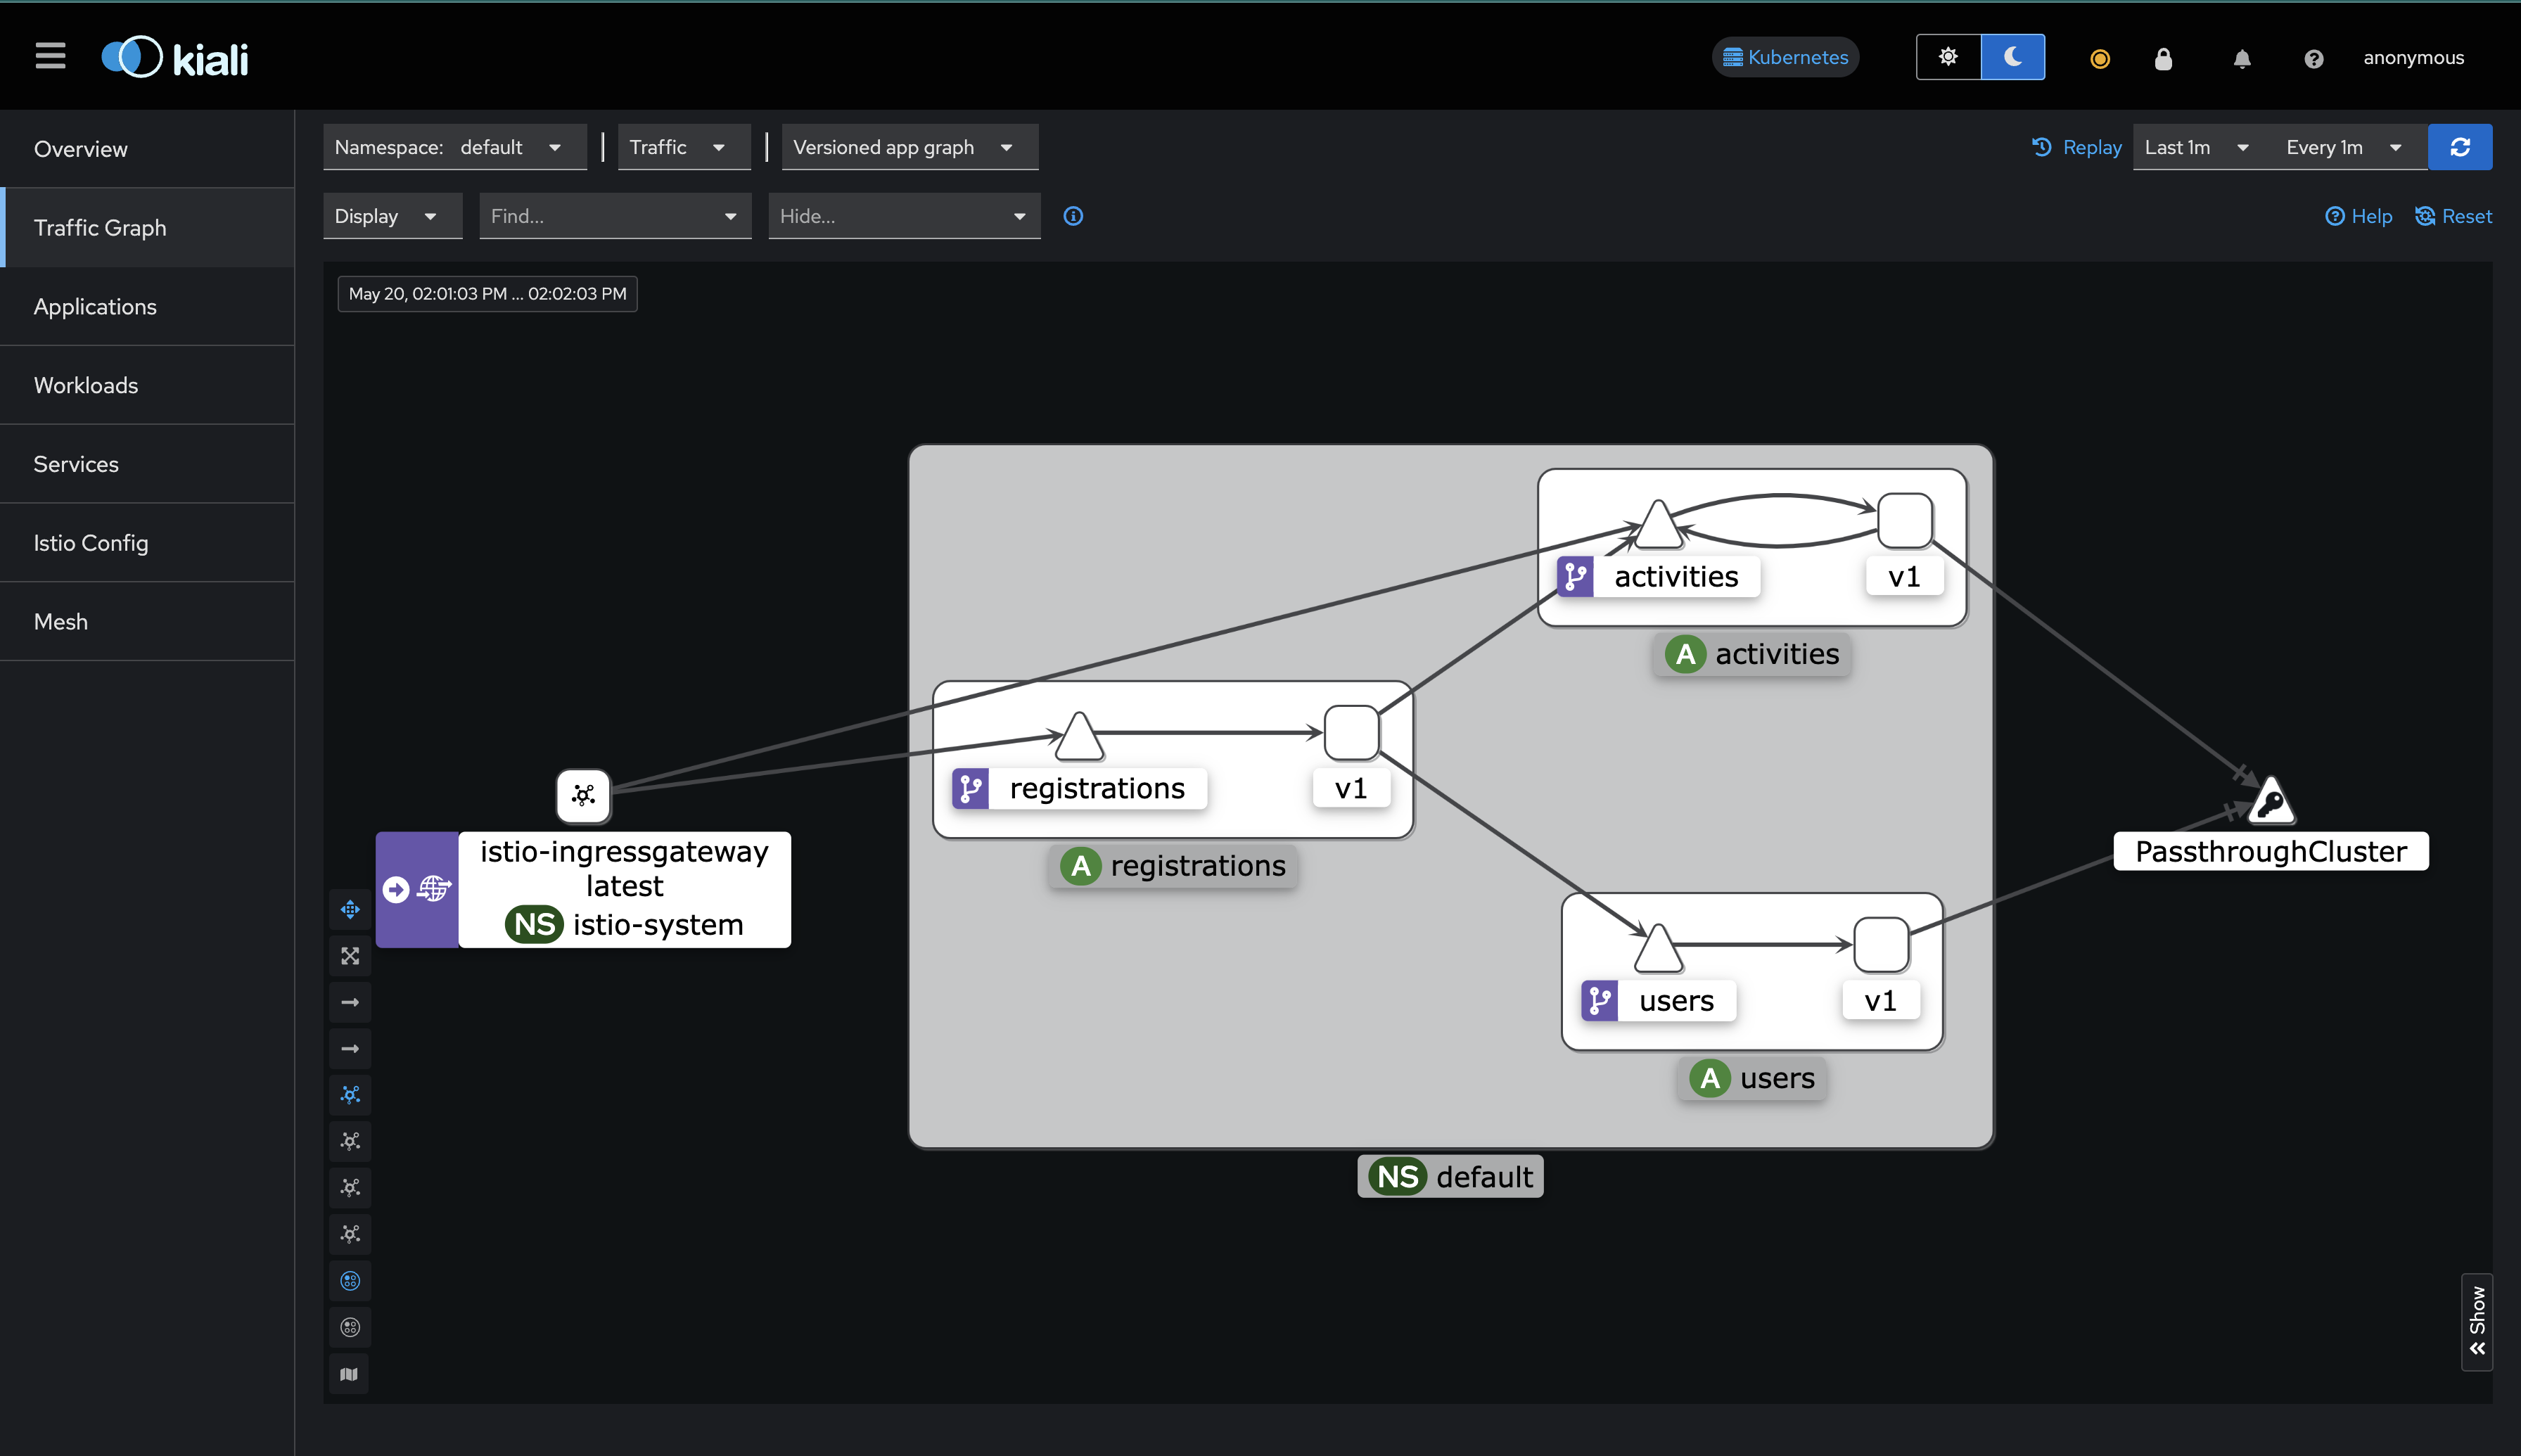
\includegraphics[width = 16cm]{kiali.png} 
    \caption{Kiali Console} 
    \label{fig:kaili}
\end{figure}

Als de activiteitenservice wordt aangeroepen, wordt deze rechtstreeks via de ingressgateway aangeroepen. In de Kiali-console wordt dit weergegeven als een directe verbinding tussen de ingressgateway en de activiteitenservice \ref{fig:kaili2}.

\begin{figure}[H]
    \centering	
    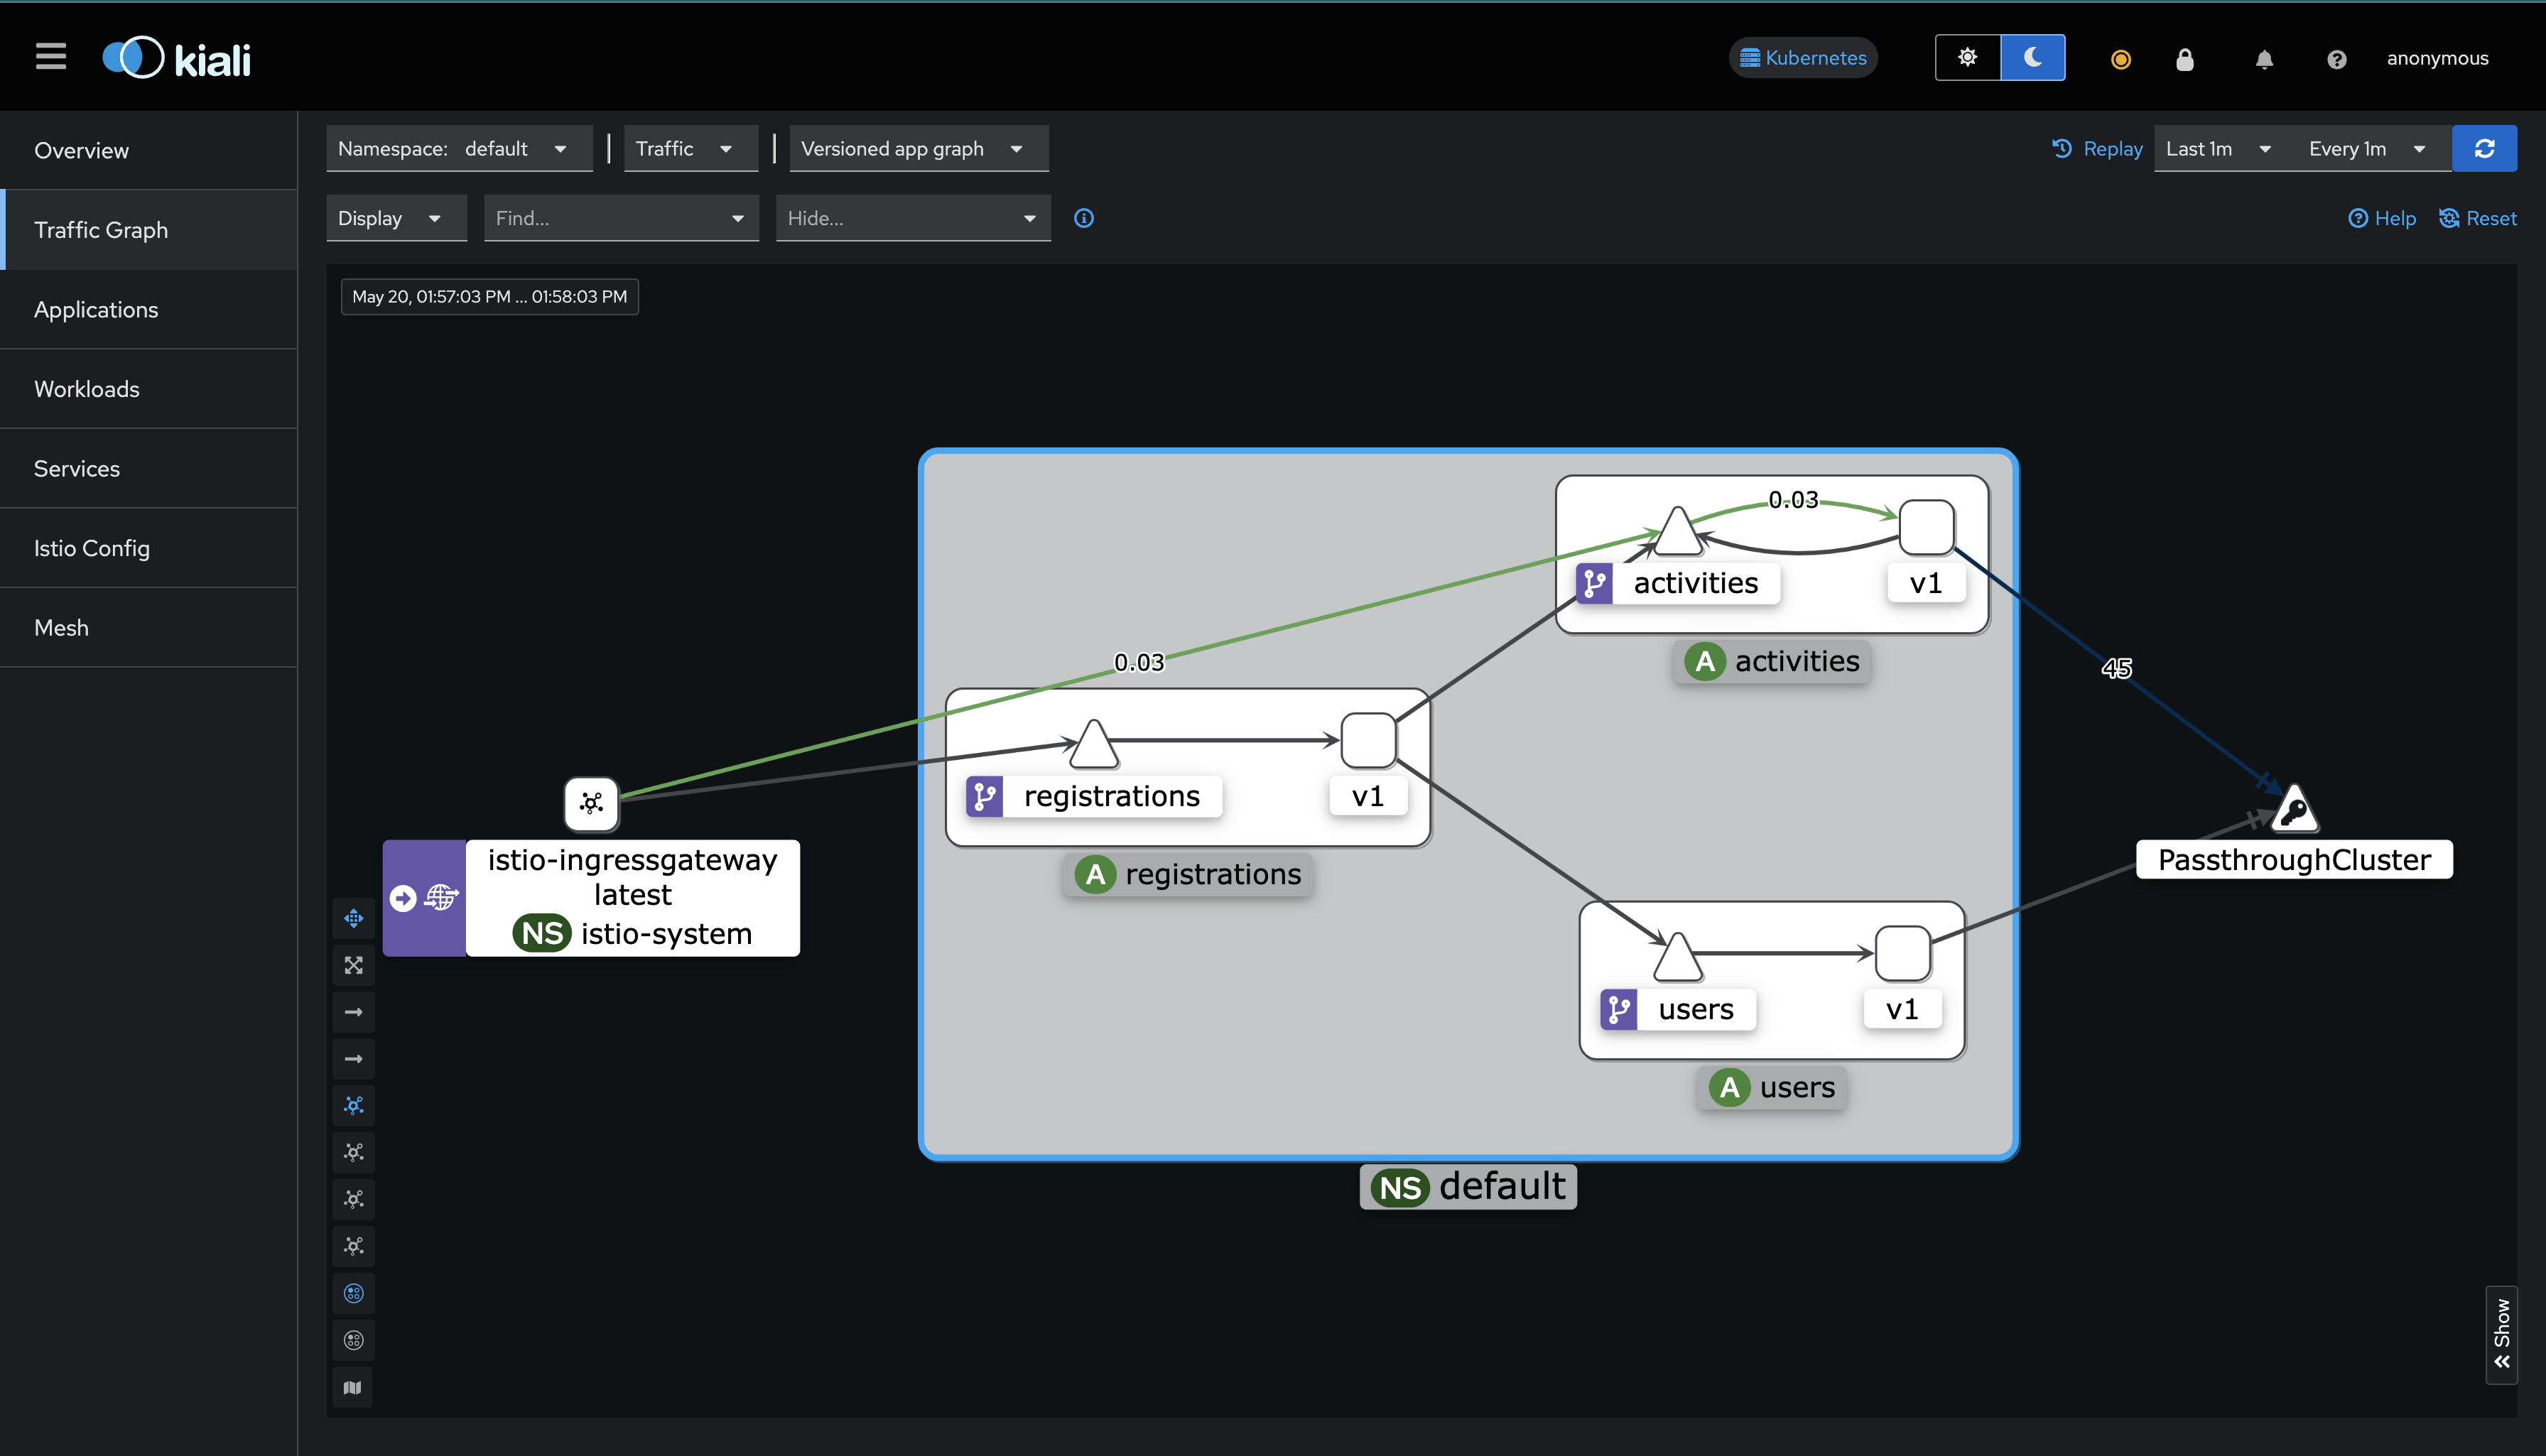
\includegraphics[width = 16cm]{kialiActivity.png} 
    \caption{Kiali Console met verkeer} 
    \label{fig:kaili2}
\end{figure}

Als de activiteit details van de registartieservice worden aangeroepen, roept de registratieservice de activiteitenservice aan. In de Kiali-console wordt dit weergegeven als een verbinding tussen de registratieservice en de activiteitenservice \ref{fig:kaili3}.

\begin{figure}[H]
    \centering	
    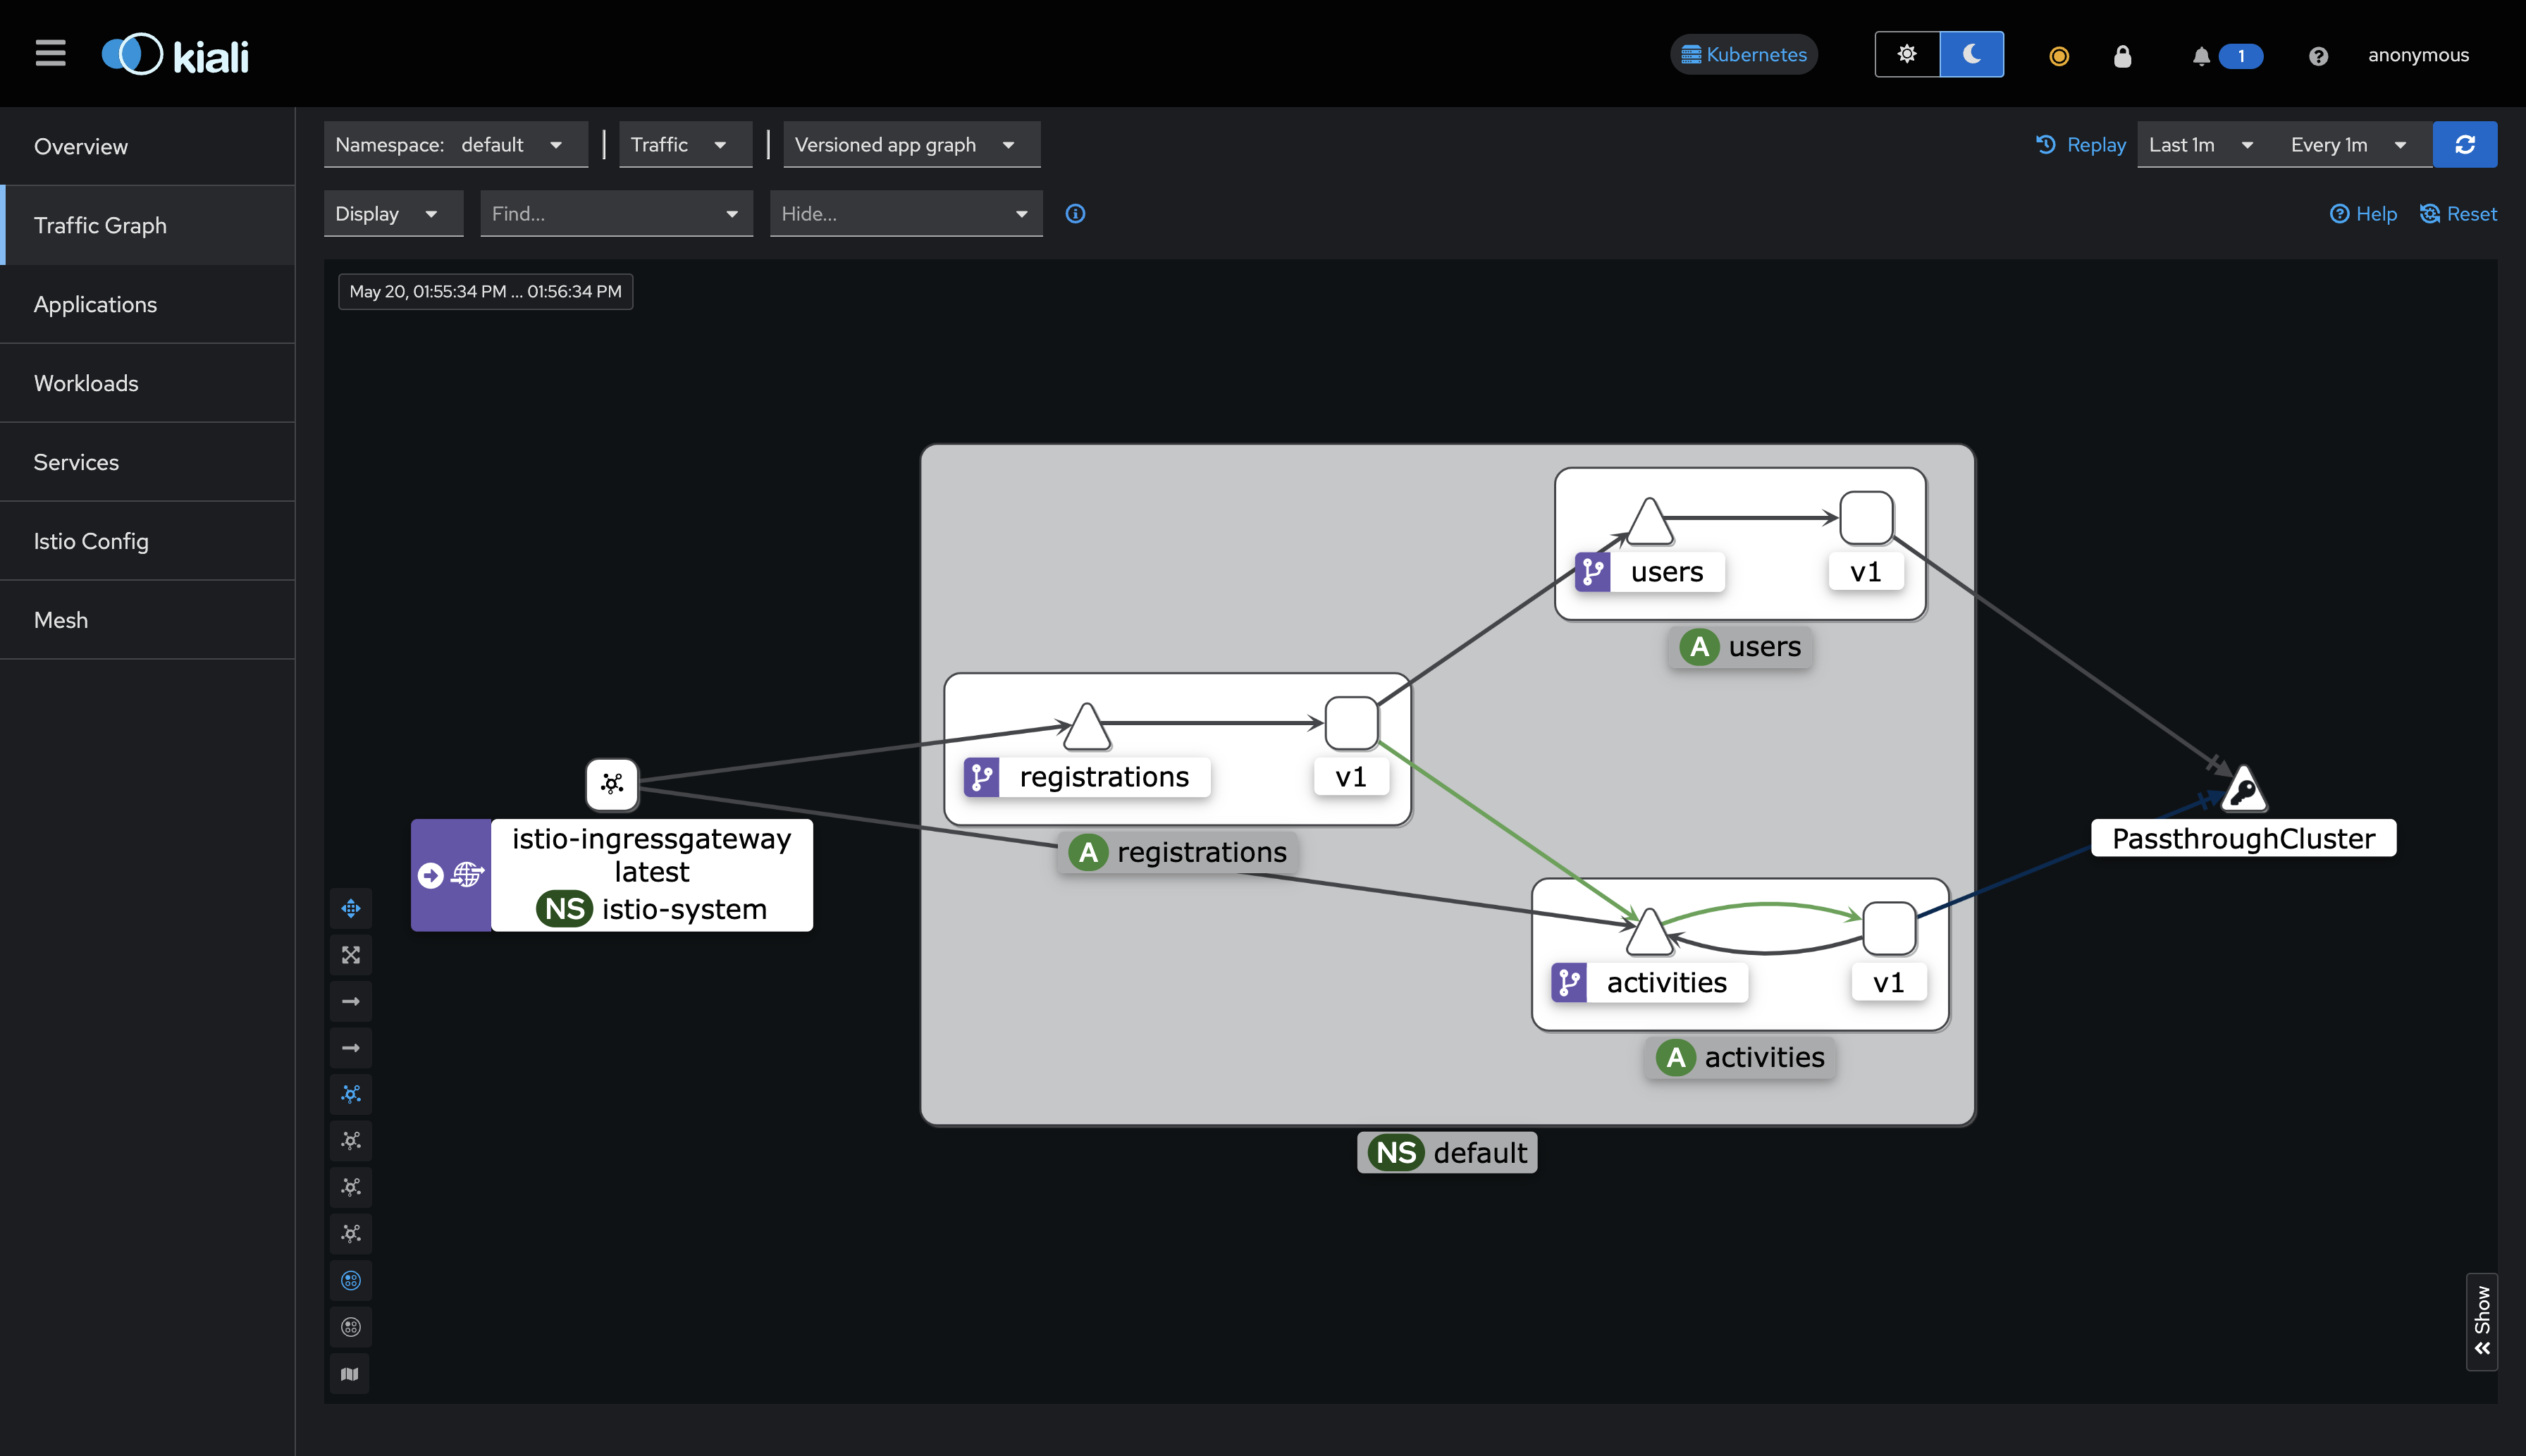
\includegraphics[width = 16cm]{kialiRegistration.png} 
    \caption{Kiali Console met verkeer} 
    \label{fig:kaili3}
\end{figure}


\chapter{\IfLanguageName{dutch}{Architectuurprincipes en prestatieanalyse}{Architecture principles and performance analysis}}
\label{ch:testen-prestatieanalyse}

\section{Inleiding}

In dit hoofdstuk worden de principes van de applicatiearchitectuur en de prestatieanalyse besproken. Voor de load testing van de applicatie wordt gebruikgemaakt van \textit{ReadyAPI}, een tool die ons in staat stelt de prestaties van de applicatie te testen door het simuleren van een groot aantal gebruikers die tegelijkertijd toegang proberen te krijgen tot de applicatie.

\section{Architectuurprincipes}

\subsection{Discoverability}

Discoverability verwijst naar het gemak waarmee de verschillende services en hun functionaliteiten kunnen worden gevonden en gebruikt binnen een microservices-architectuur. Dit aspect is cruciaal voor de efficiëntie en het onderhoud van de applicatie, aangezien het helpt bij het snel identificeren van de juiste services voor specifieke taken.

Er zijn 2 aspecten van discoverability die belangrijk zijn bij het ontwerpen van een microservices architectuur. Het technische aspect verwijst naar het vermogen van services om elkaar te vinden en met elkaar te communiceren binnen een netwerk. Het operationele aspect verwijst naar het vermogen van ontwikkelaars en beheerders om de services te vinden en te begrijpen.

Om een call te doen naar een andere service moet enkel de naam van de service en de poort waarop deze draait gekend zijn. Dit is mogelijk door de service discovery van Istio. Hierdoor kunnen services elkaar vinden en met elkaar communiceren zonder dat de locatie van de service gekend moet zijn.

Voor het operationele aspect bieden de meeste servicemeshes een dashboard aan waarin de services en hun interacties visueel worden weergegeven. Dit maakt het gemakkelijk voor ontwikkelaars en beheerders om de services te vinden en te begrijpen. In Istio is dit het Kiali-dashboard \ref{fig:kaili} \ref{fig:kialiServices}.

\begin{figure}[H]
    \centering	
    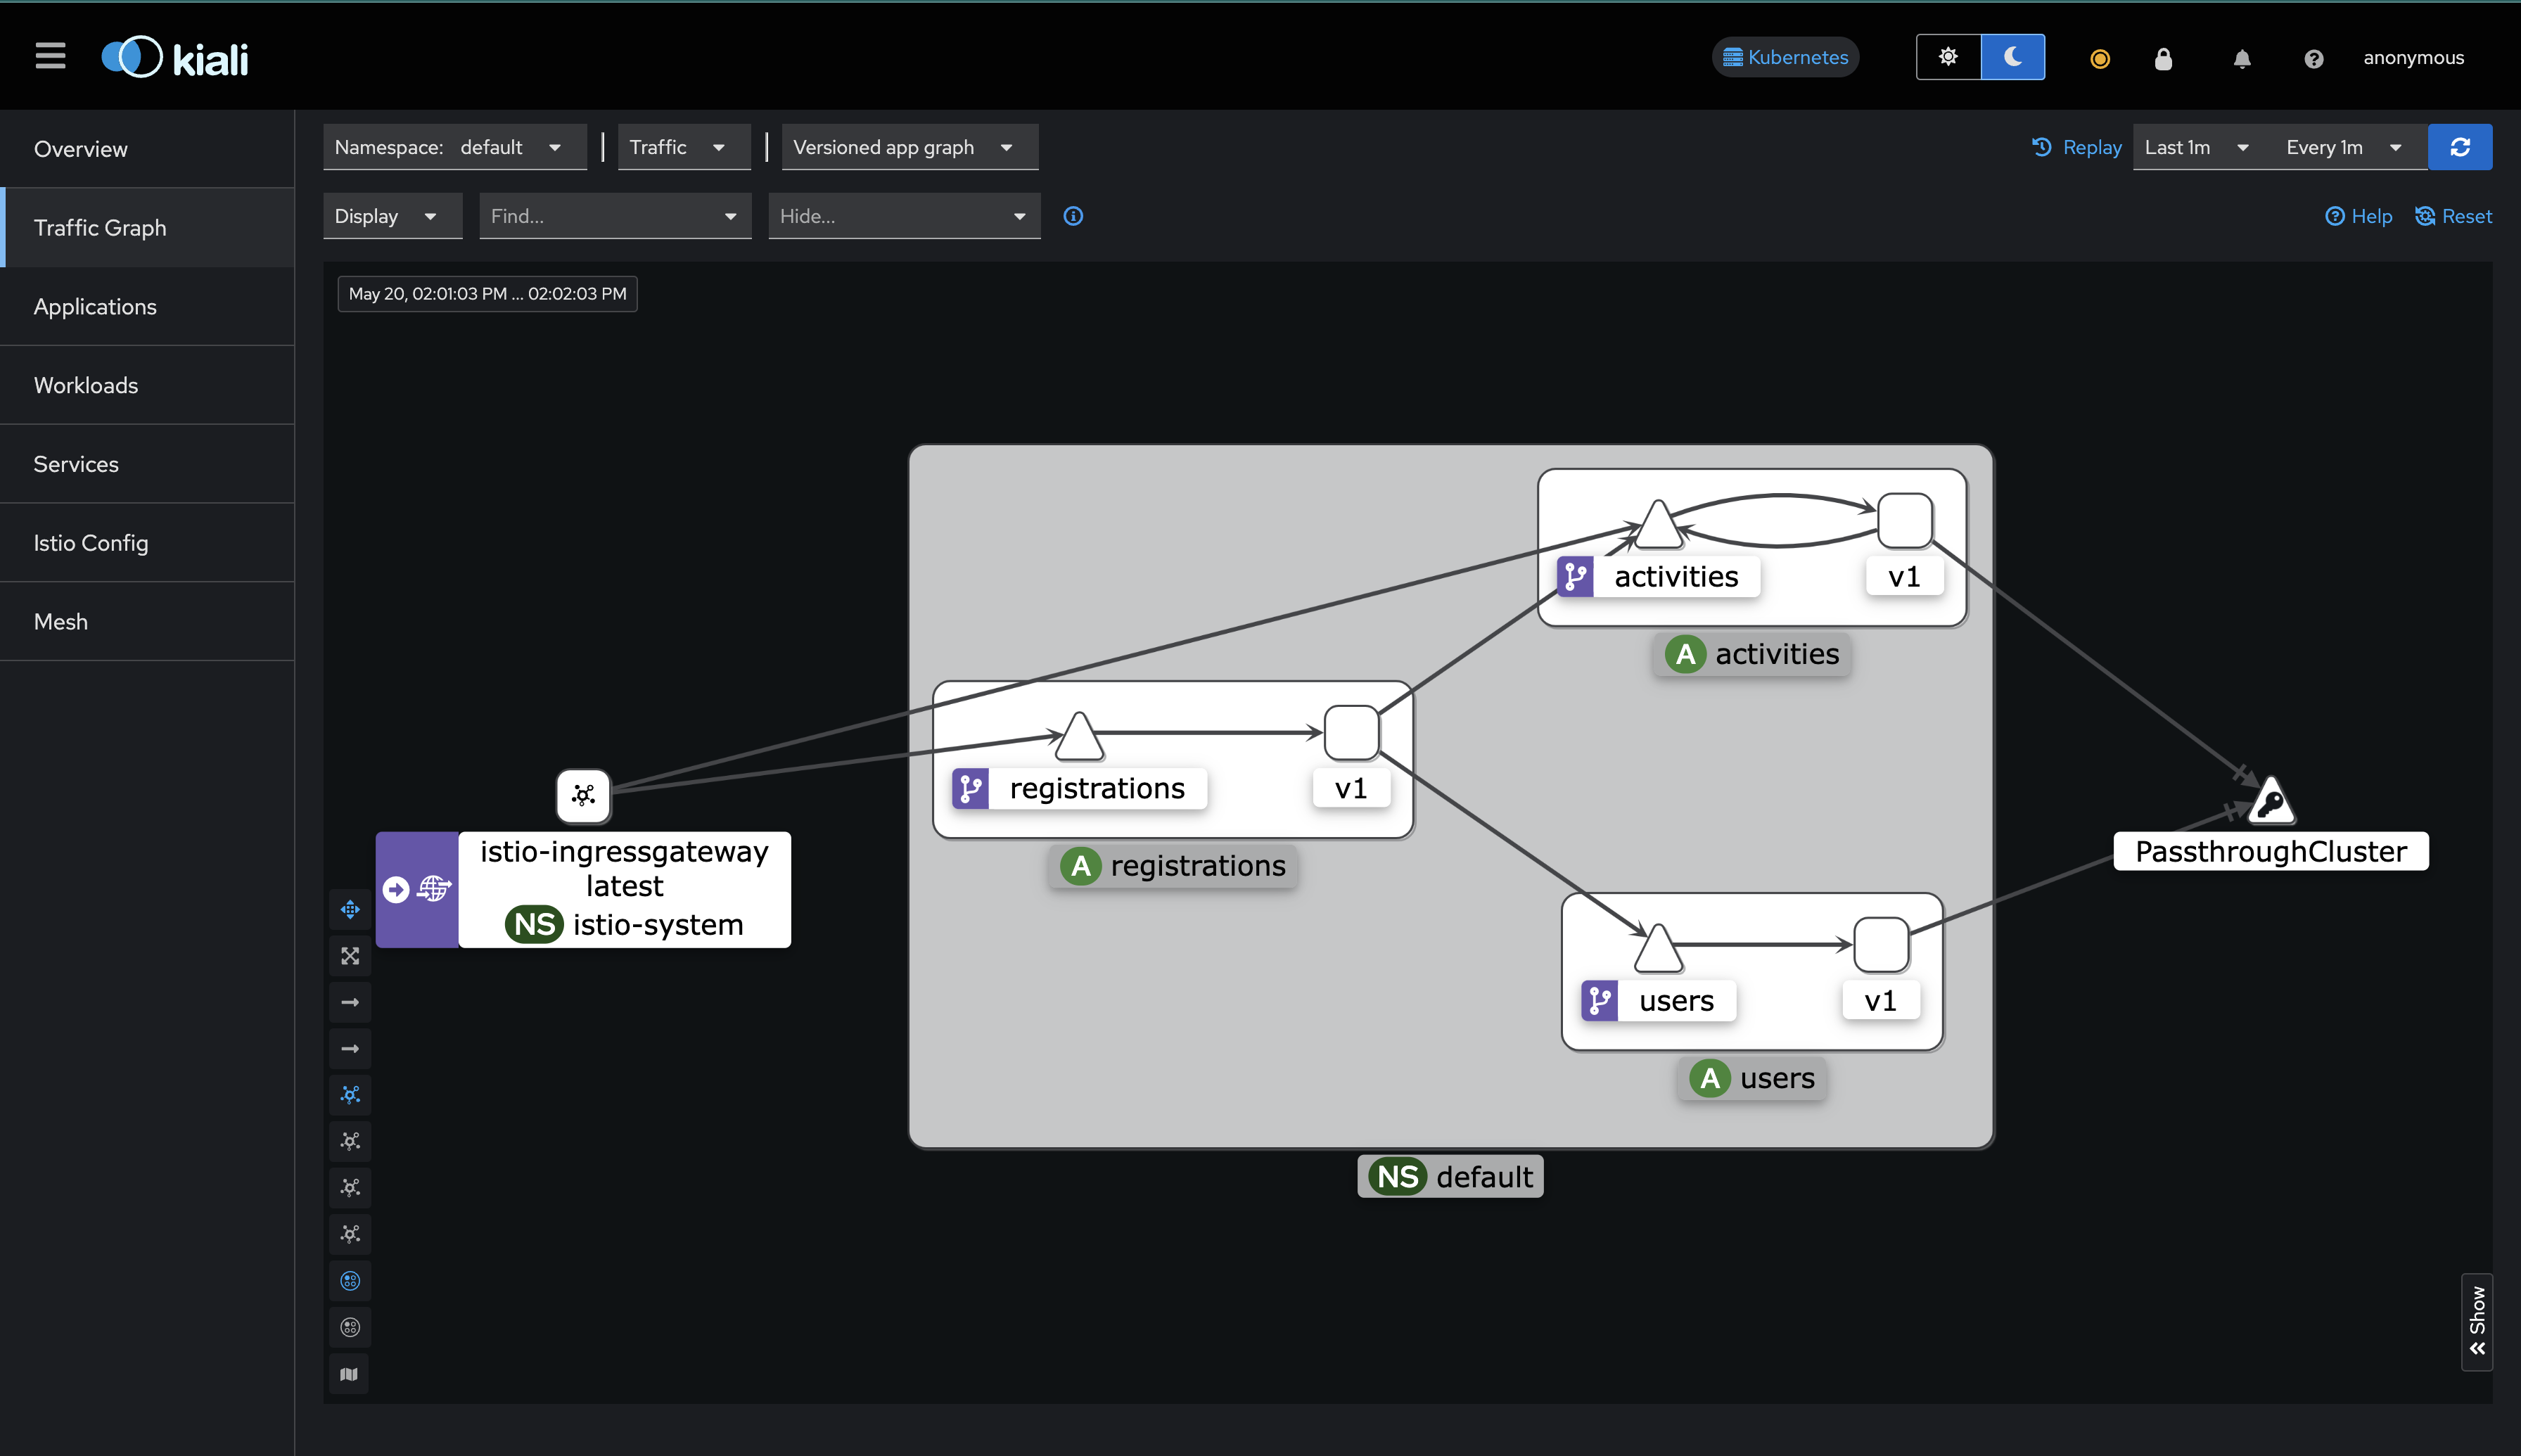
\includegraphics[width = 16cm]{kiali.png} 
    \caption{Kiali Console} 
    \label{fig:kaili}
\end{figure}

\begin{figure}[H]
    \centering	
    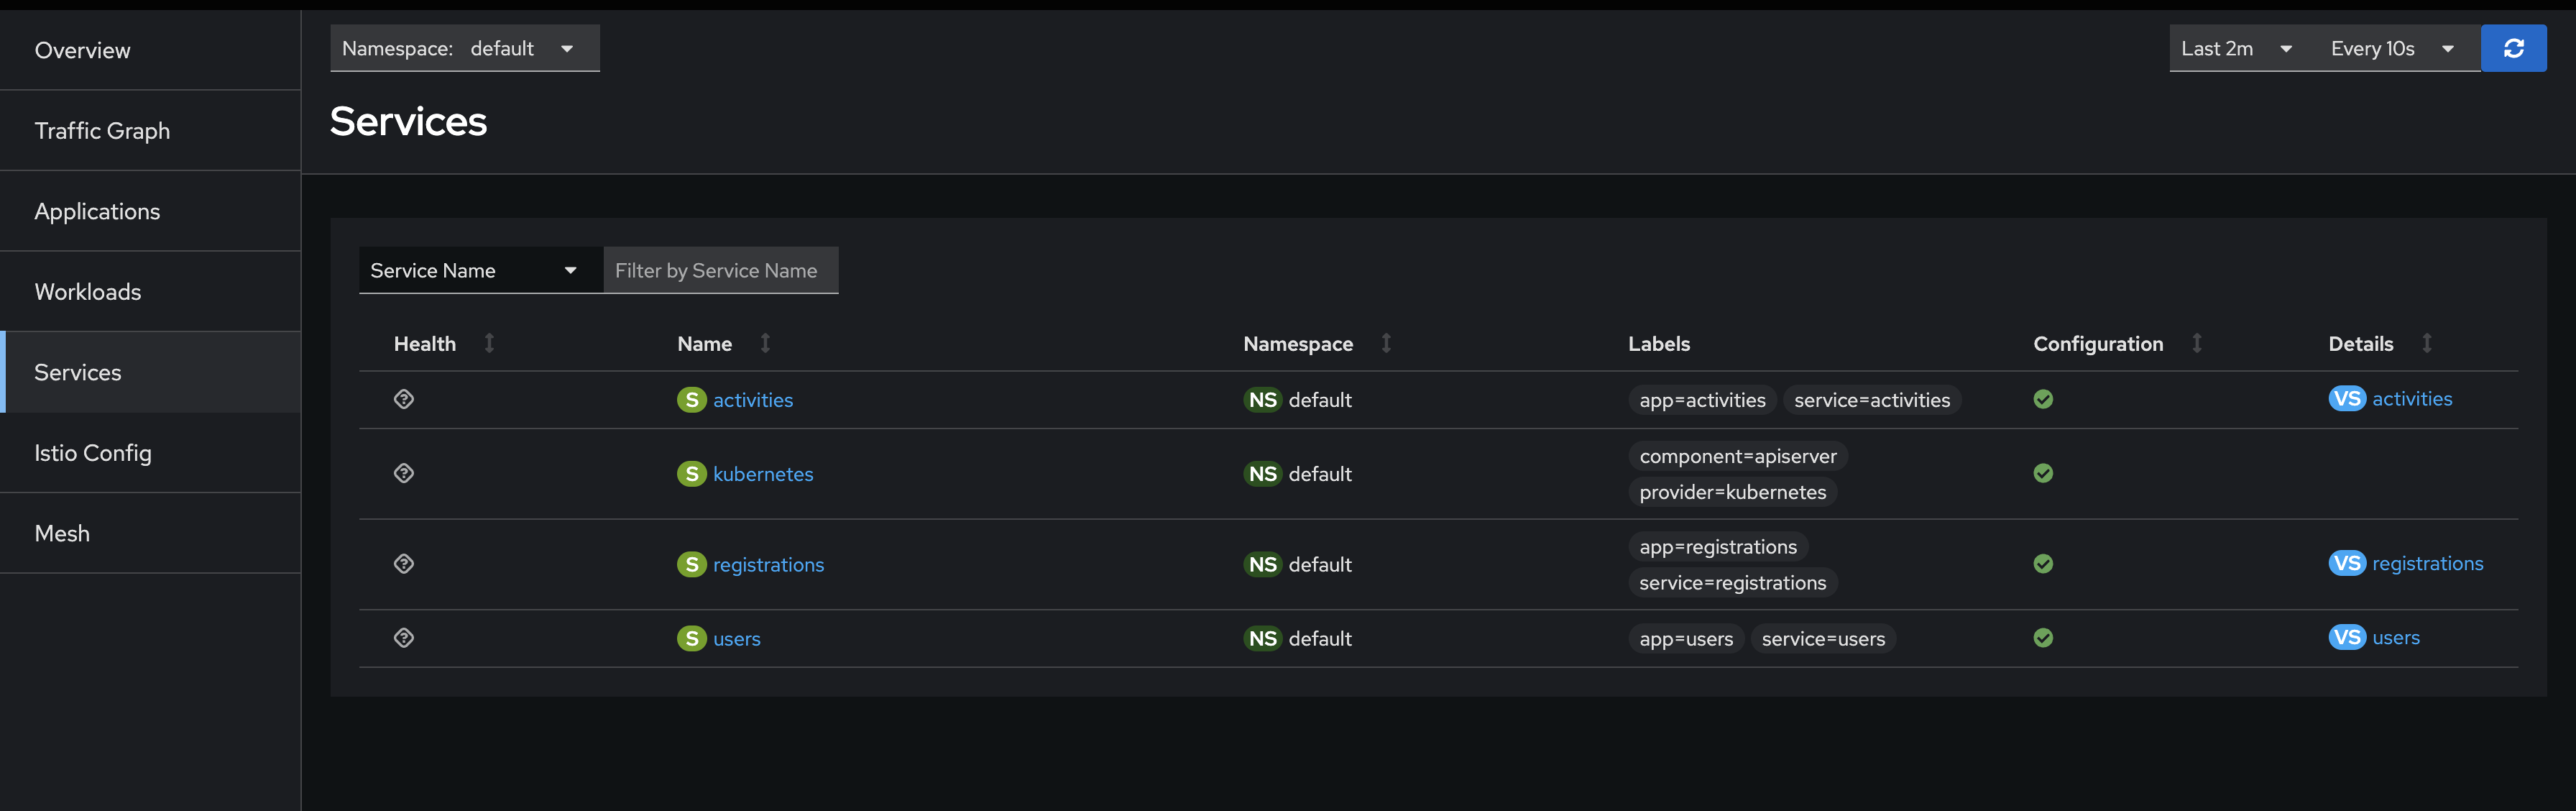
\includegraphics[width = 16cm]{kialiServices.png} 
    \caption{Kiali Console met services} 
    \label{fig:kialiServices}
\end{figure}


\subsection{Schaalbaarheid}

Schaalbaarheid is een belangrijke eigenschap van microservices, omdat ze onafhankelijk van elkaar kunnen worden geschaald. Dit betekent dat we de resources van elke service afzonderlijk kunnen verhogen om de prestaties van de applicatie te verbeteren. Door het aantal replica's van een service te verhogen, kunnen we de belasting verdelen over meerdere instanties en zo de prestaties van de applicatie verbeteren.

Om de schaalbaarheid te testen, hebben we simulaties uitgevoerd met verschillende aantallen replica's: 1, 2 en 10. De resultaten van deze tests zijn weergegeven in de figuren \ref{fig:1replica}, \ref{fig:2replica}   en \ref{fig:10replica}.

\begin{figure}[H]
    \centering	
    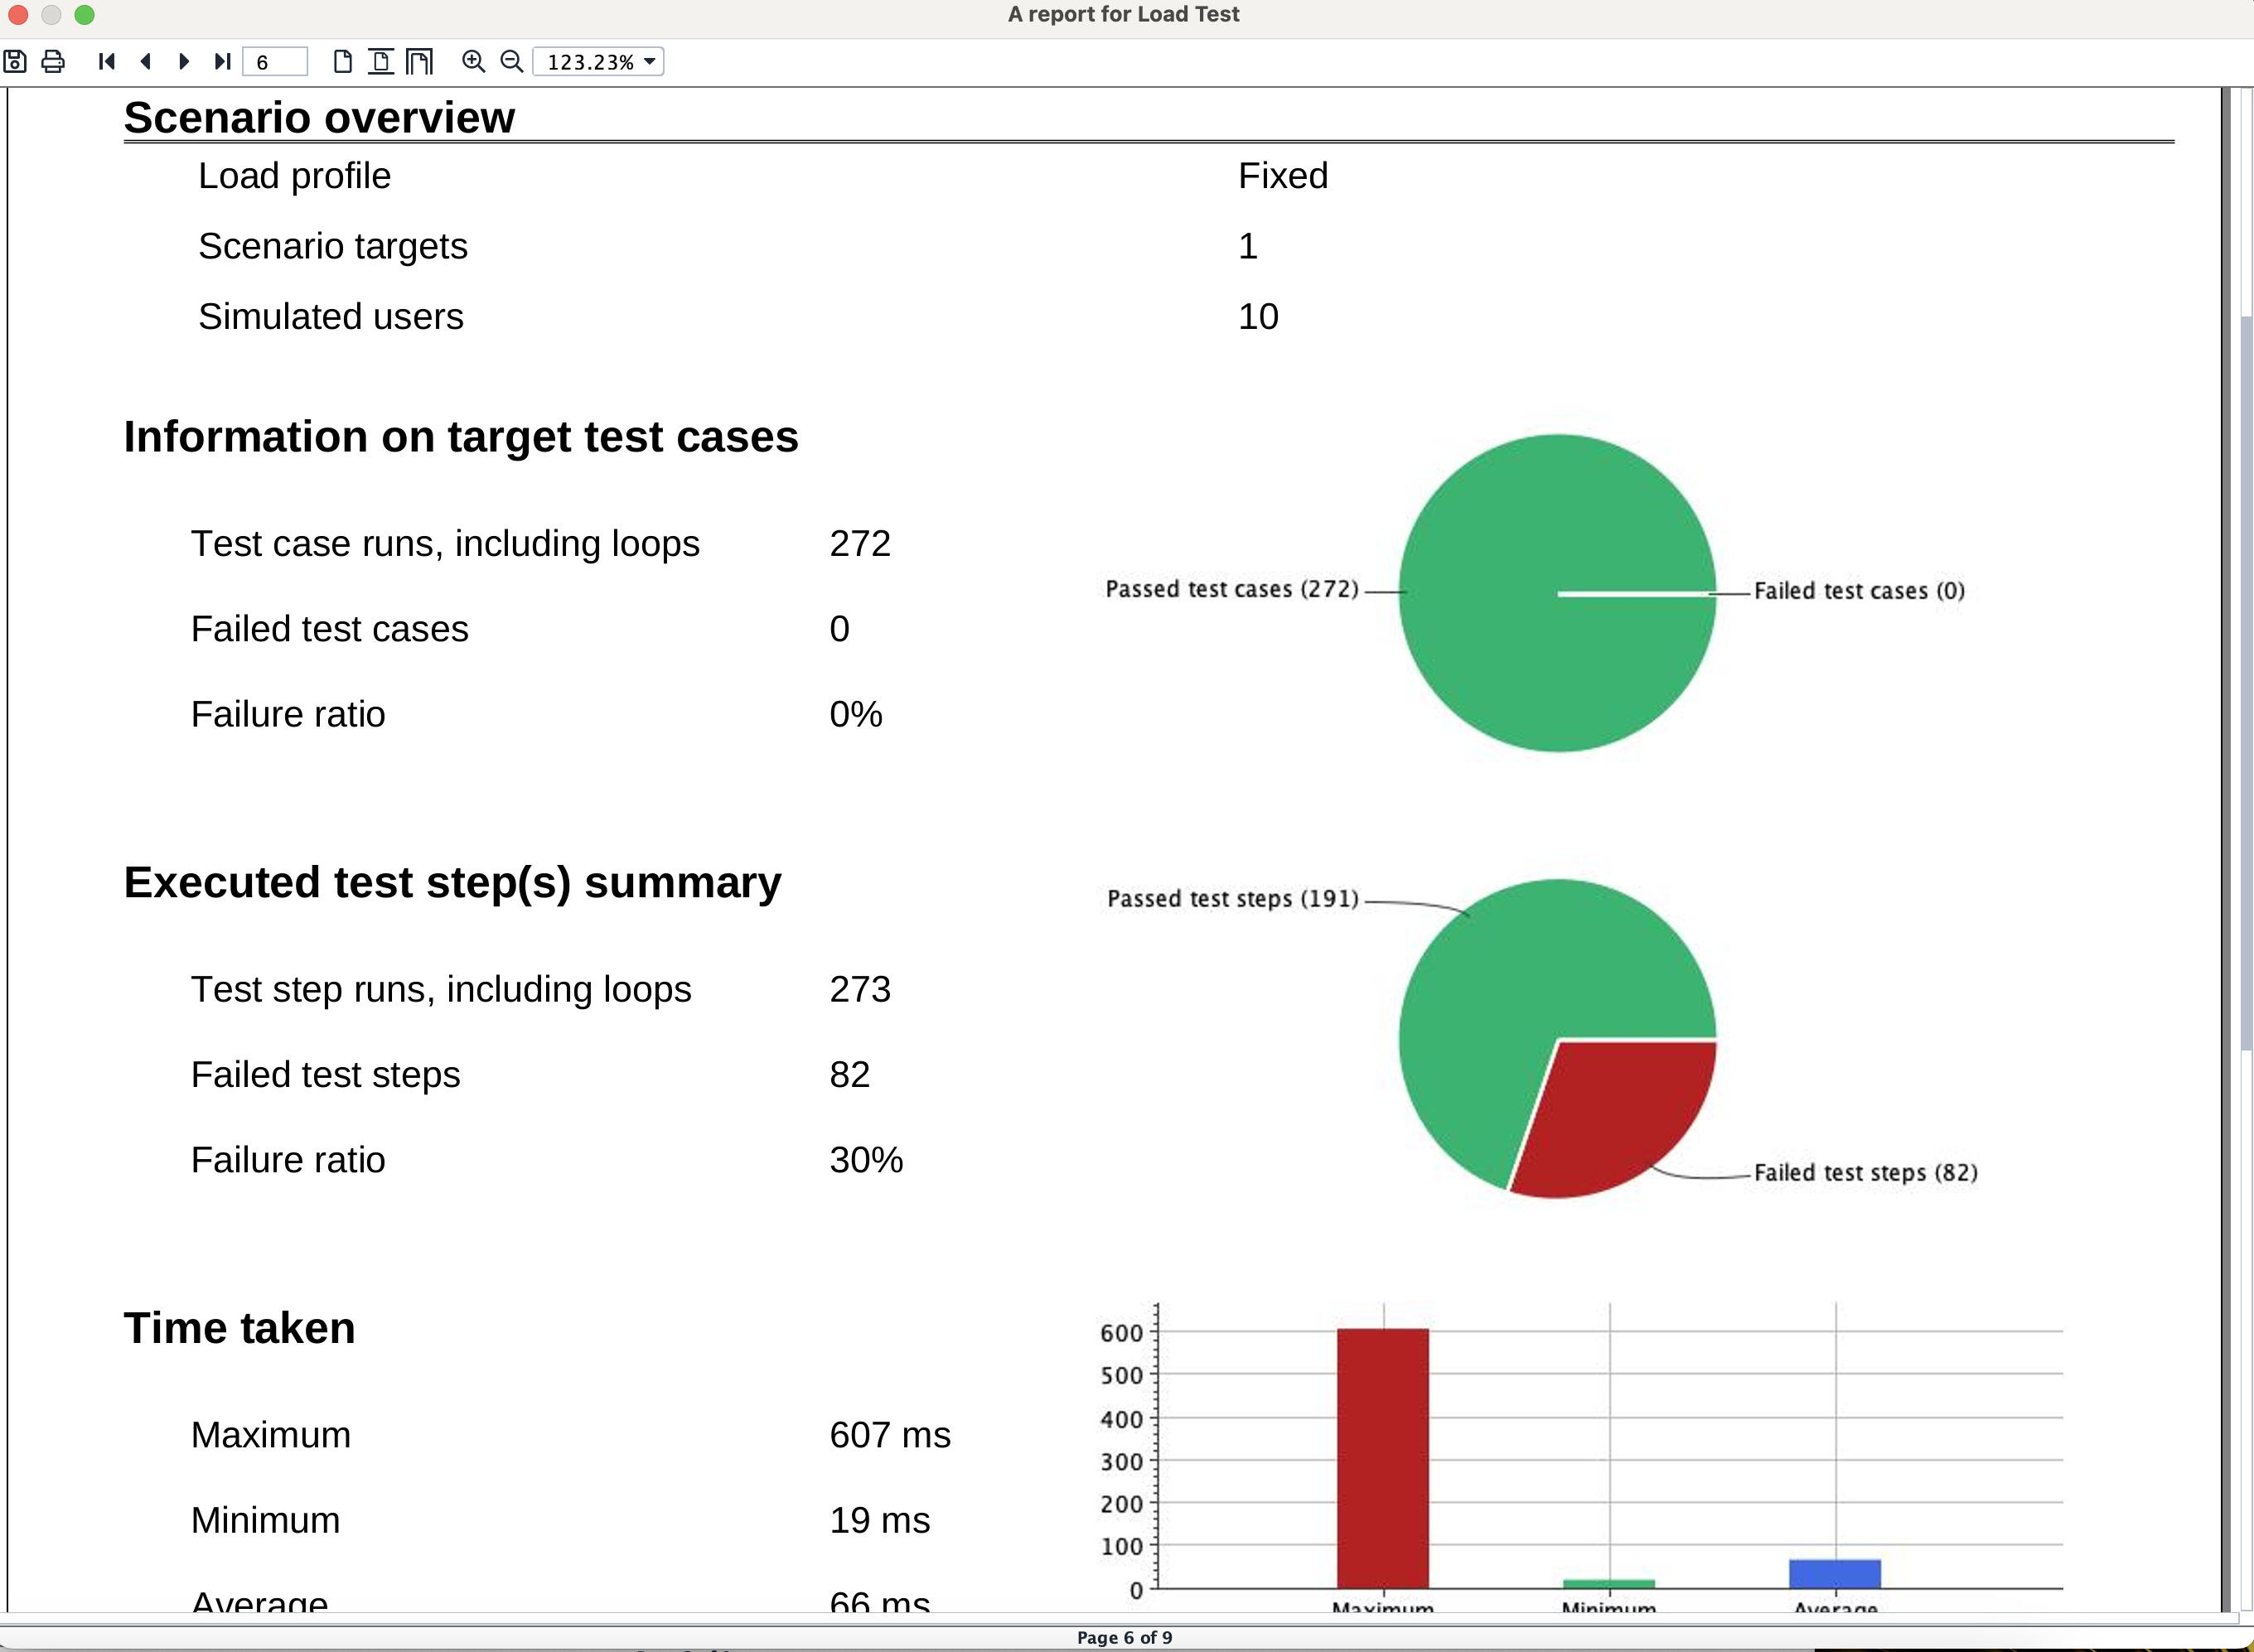
\includegraphics[width=12cm]{10sim1rep.png}
    \caption{10 simulaties op 1 replica} 
    \label{fig:1replica}
\end{figure}

\begin{figure}[H]
    \centering	
    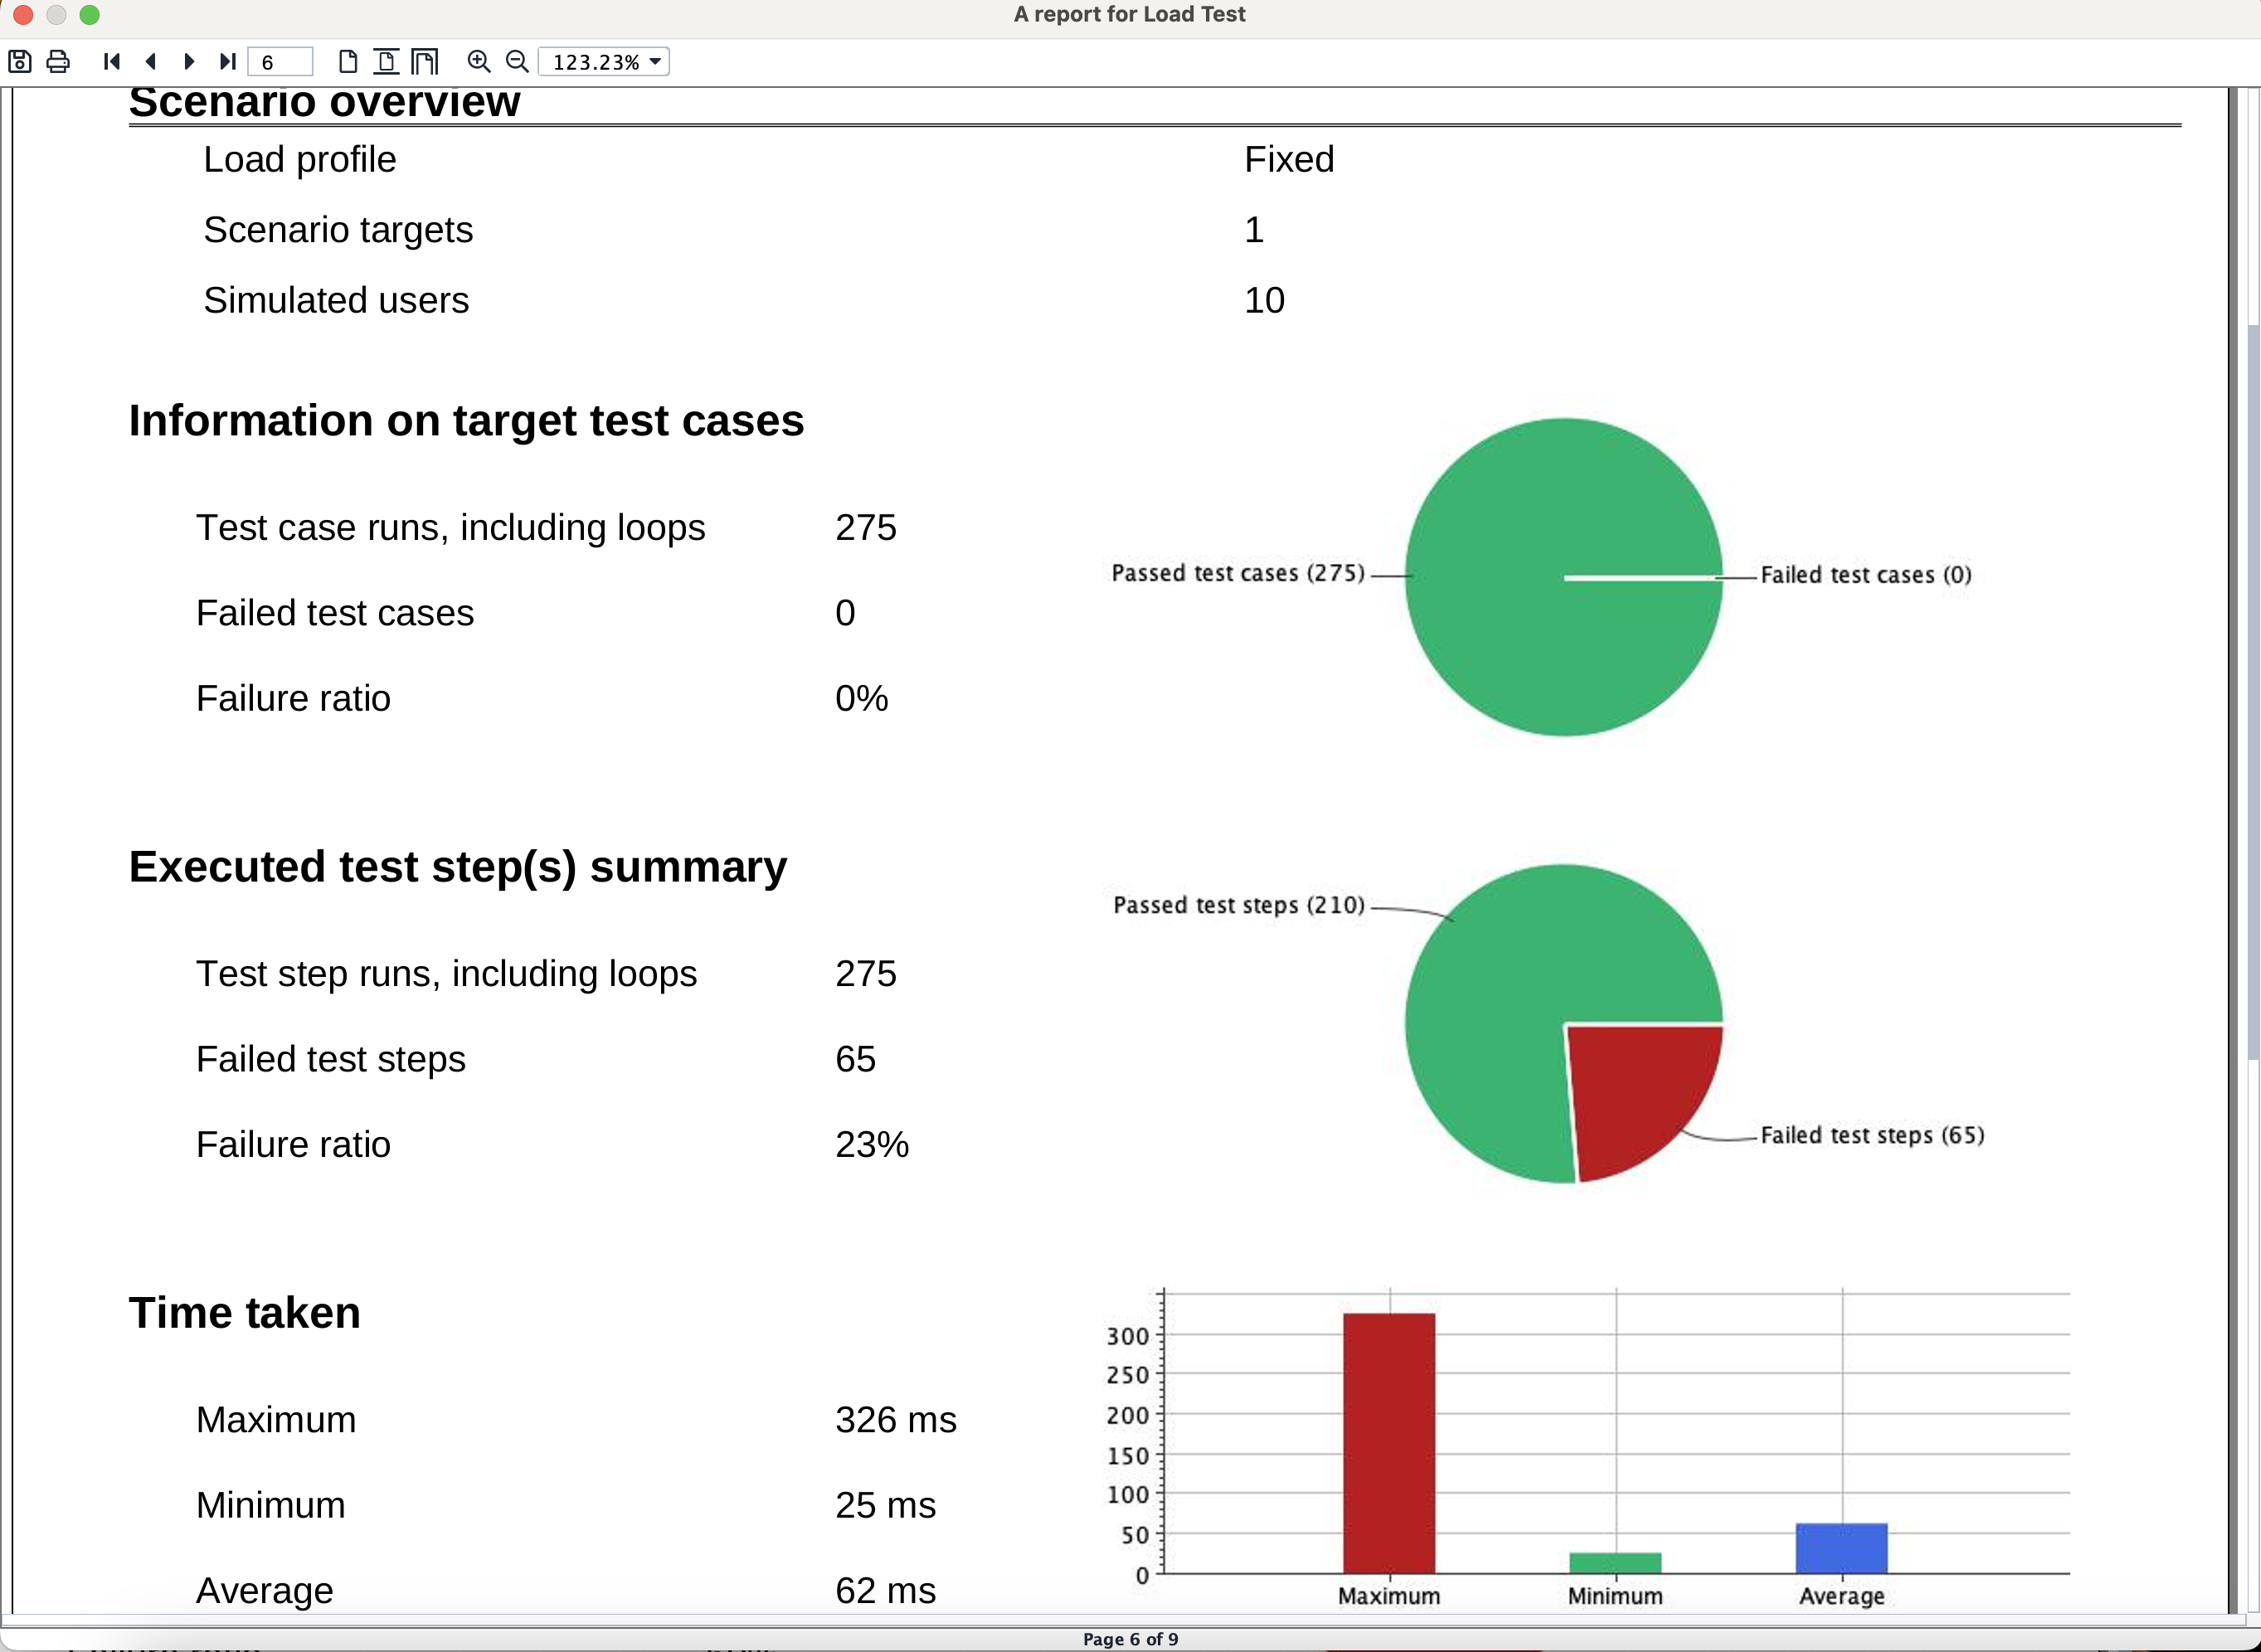
\includegraphics[width=12cm]{10sim2rep.png}
    \caption{10 simulaties op 2 replica's} 
    \label{fig:2replica}
\end{figure}

\begin{figure}[H]
    \centering	
    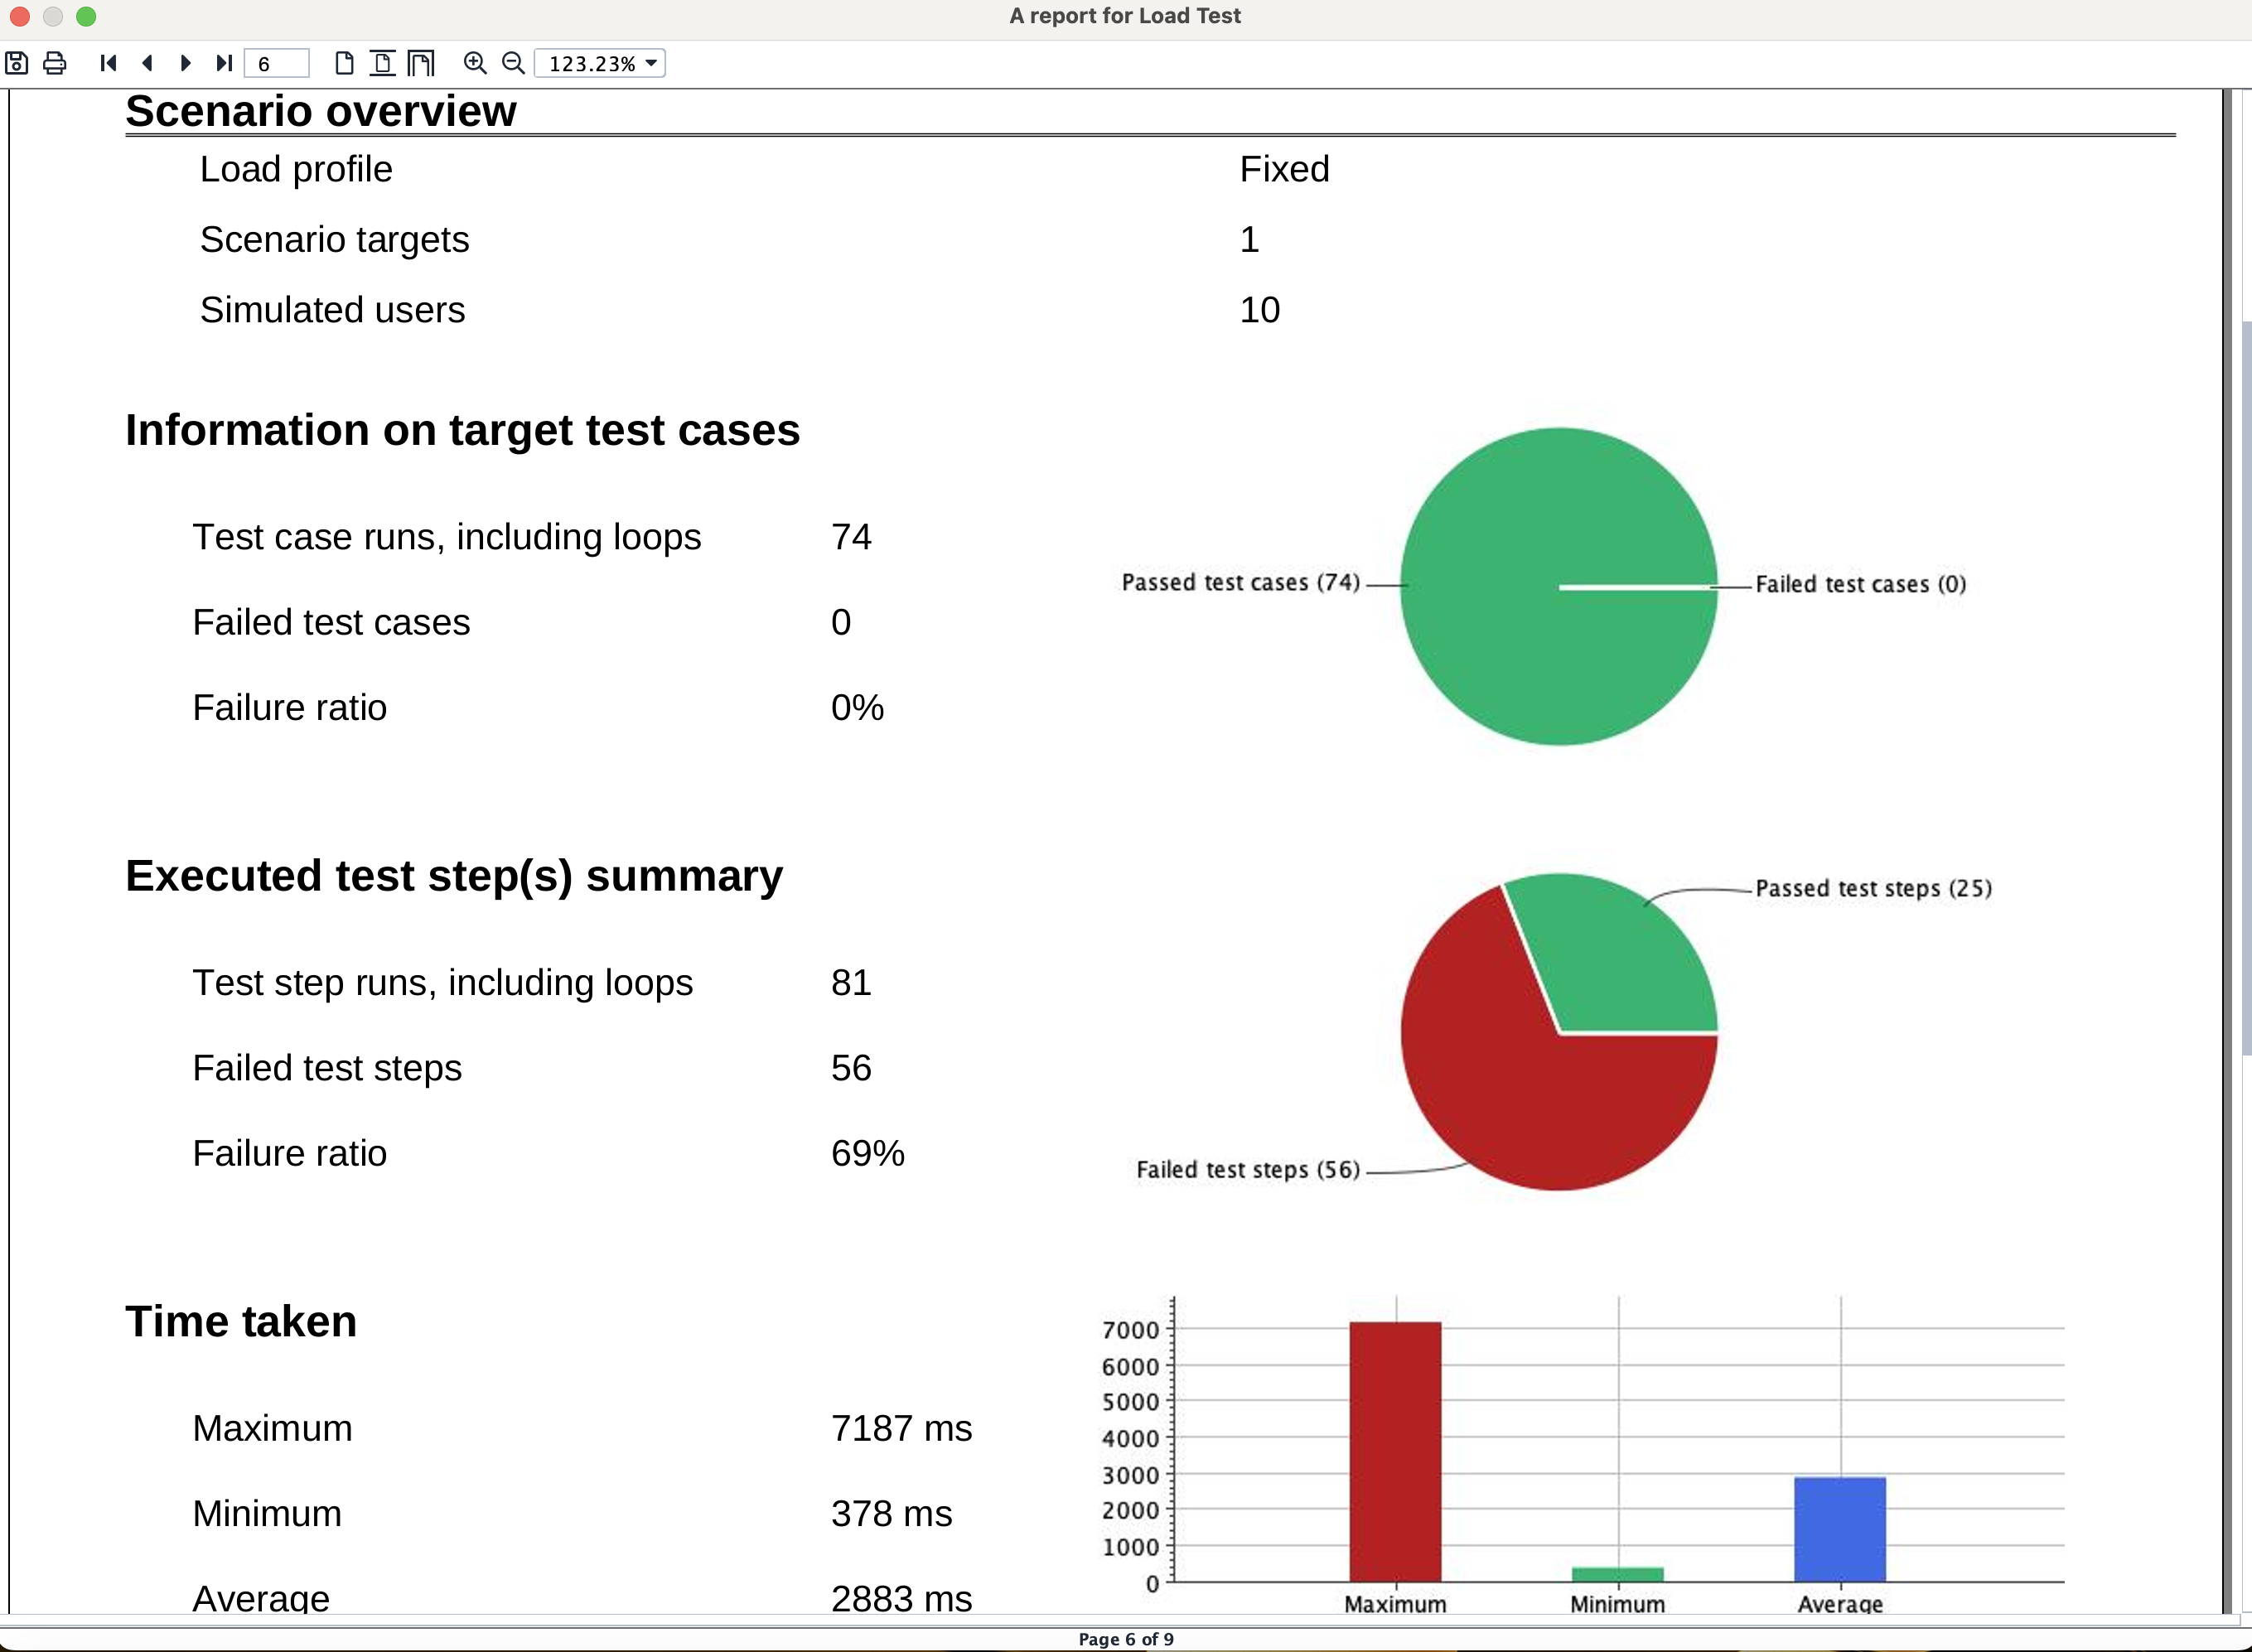
\includegraphics[width=12cm]{10sim10rep.png}
    \caption{10 simulaties op 10 replica's} 
    \label{fig:10replica}
\end{figure}

Uit de resultaten blijkt dat bij het verhogen van het aantal replica's de prestaties verbeteren tot een bepaald punt. Bij 2 replica's zijn de testsuccespercentages hoger en zijn er minder time-outs. 

Bij het draaien van 10 replica's zijn de recources van mijn desktop overbelast. Er is wel te zien dat bij het opschalen van de replica's de prestaties verbeteren tot het punt waarop de infrastructuur overbelast raakt.

Dit komt omdat mijn infrastructuur (desktop) niet mee kan schalen met het aantal replica's wat in een professionele omgeving wel zou kunnen.

Theoretisch zijn microservices oneindig horizontaal schaalbaar, terwijl monolieten meestal enkel verticaal schaalbaar zijn. Dit beperkt de schaalbaarheid van monolieten tot de maximale grootte van de servers waarop ze draaien.

Verticaal schalen is meer kracht aan de server toevoegen, terwijl horizontaal schalen het toevoegen van meer servers is.


\section{Prestatieanalyse}

\subsection{Responstijd}

De responstijd is een kritieke prestatie-indicator voor de applicatie. Voor het testen van de responstijd hebben we gebruikgemaakt van \textit{ReadyAPI} om zowel een monolithische versie van de applicatie als de microservices-versie te testen. De resultaten zijn weergegeven in de figuren \ref{fig:monolietTimeTest} en \ref{fig:microservicesTimeTest}.

\subsubsection*{Health check - single threaded}

Als eerste test wordt een single threaded health check uitgevoerd op beide systemen. Hiermee wordt gekeken wat de impact is van de architectuur op de responstijd van de applicatie. De resultaten van deze test zijn weergegeven in de figuren \ref{fig:monolietTimeHealth} en \ref{fig:microservicesTimeHealth}.

\begin{figure}[H]
    \centering	
    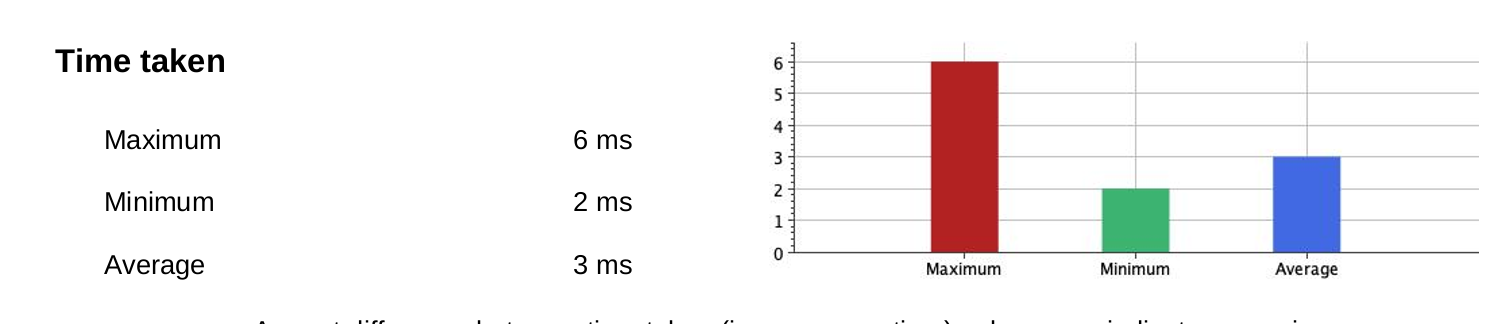
\includegraphics[width=12cm]{monolietTimeHealth.png}
    \caption{Responstijd monoliet health check} 
    \label{fig:monolietTimeHealth}
\end{figure}

\begin{figure}[H]
    \centering	
    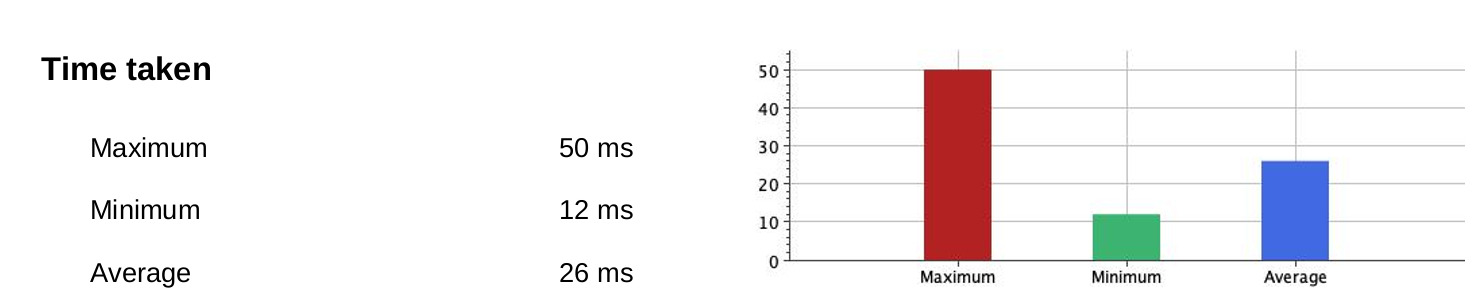
\includegraphics[width=12cm]{microservicesTimeHealth.png}
    \caption{Responstijd microservices health check} 
    \label{fig:microservicesTimeHealth}
\end{figure}

Uit de resultaten blijkt dat de responstijd van de monoliet lager is dan die van de microservices. Bij de monoliet applicatie wordt rechtstreeks een HTTP call gedaan naar de API, terwijl bij de microservices de API calls worden gedaan via een ingressgateway, sidecar proxy en dan pas naar de API. Dit verklaart waarschijnlijk waarom de responstijd van de microservices hoger is dan die van de monoliet.
\subsubsection*{Health check - multi threaded}
Als volgende test wordt een multi-threaded health check uitgevoerd op beide systemen. Hiermee wordt gekeken wat de impact is van de architectuur op de responstijd van de applicatie. De resultaten van deze test zijn weergegeven in de figuren \ref{fig:monolietTimeHealthMulti} en \ref{fig:microservicesTimeHealthMulti}.

\begin{figure}[H]
    \centering	
    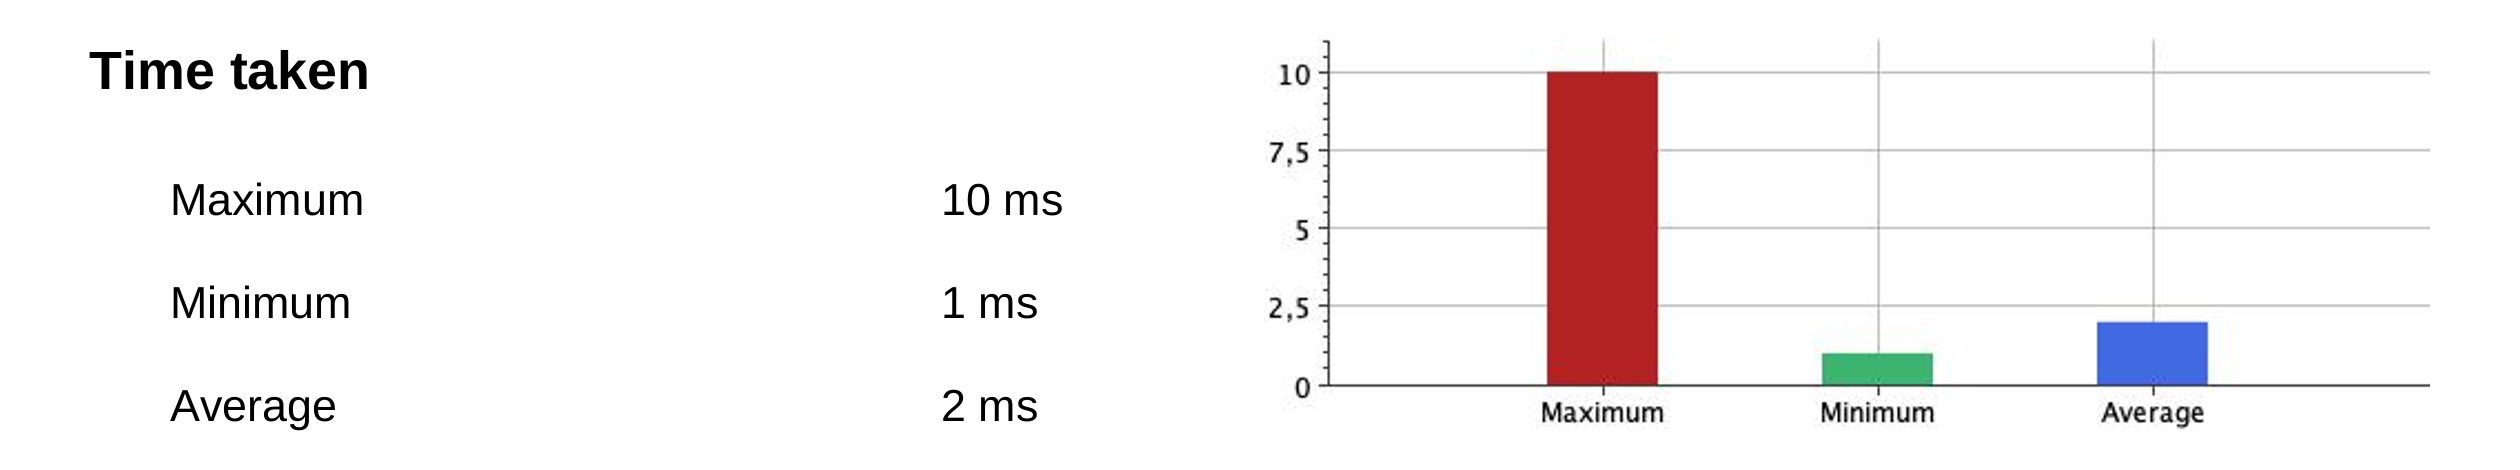
\includegraphics[width=12cm]{monolietTimeHealthMulti.png}
    \caption{Responstijd monoliet health check multi-threaded} 
    \label{fig:monolietTimeHealthMulti}
\end{figure}

\begin{figure}[H]
    \centering	
    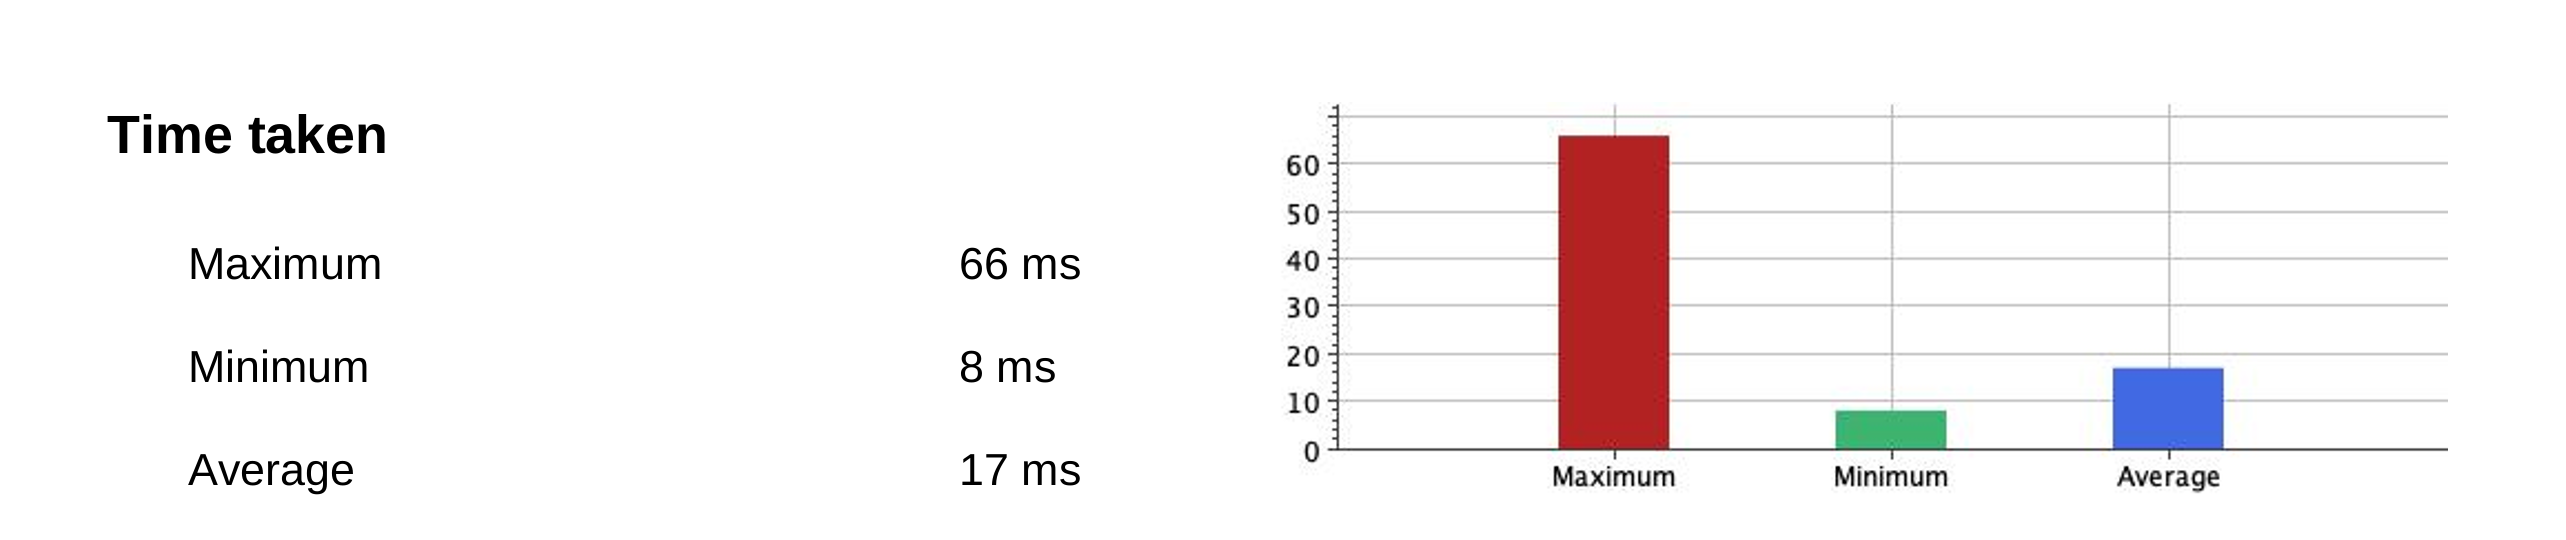
\includegraphics[width=12cm]{microservicesTimeHealthMulti.png}
    \caption{Responstijd microservices health check multi-threaded} 
    \label{fig:microservicesTimeHealthMulti}
\end{figure}

Er is dus geen significant verschil in responstijd bij een multi-threaded health check ten opzichte van single threaded. Het lijkt dus dat beide architecturen hetzelfde aantal requests aankunnen.
\subsubsection*{Service to service invocation}
Als laatste test wordt een api aangeroepen die de registraties voor een activiteit ophaalt samen met de details van de activiteit. Hiermee wordt gekeken wat de impact is van de architectuur op de responstijd van de applicatie. De resultaten van deze test zijn weergegeven in de figuren \ref{fig:monolietTimeTest} en \ref{fig:microservicesTimeTest}.

In de monoliet wordt dit gedaan door een join in de repository laag, terwijl in de microservice de registratieservice de activiteitenservice aanroept.

\begin{figure}[H]
    \centering	
    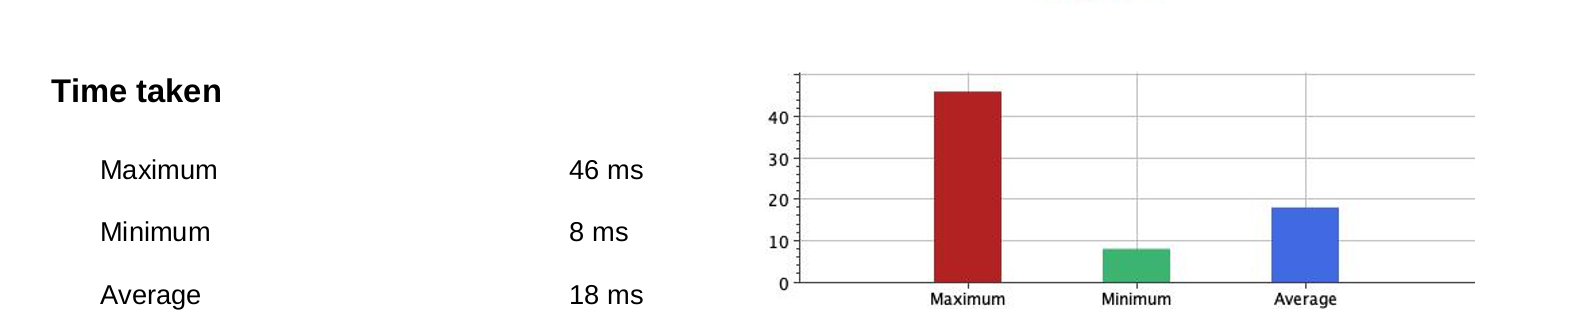
\includegraphics[width=12cm]{monolietTimeTest.png}
    \caption{Responstijd monoliet} 
    \label{fig:monolietTimeTest}
\end{figure}

\begin{figure}[H]
    \centering	
    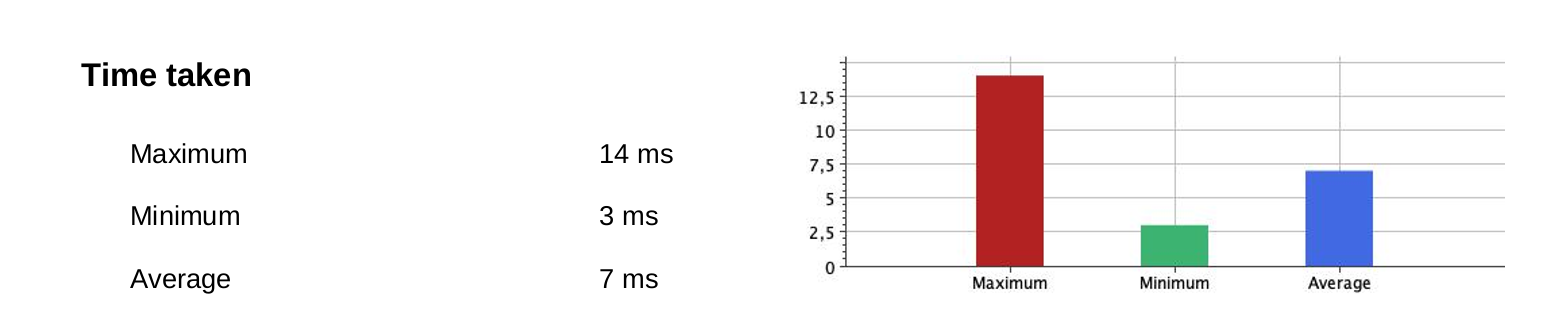
\includegraphics[width=12cm]{microservicesTimeTest.png}
    \caption{Responstijd microservices} 
    \label{fig:microservicesTimeTest}
\end{figure}

Er is geen significant verschil tussen de responstijden in deze testen en de voorafgaande testen. Het lijkt dus dat de service to service calls minder impact hebben op de response tijd dan de ingress calls. Om deze calls zoveel mogelijk te beperken zou de UI zelf of een facade service voor de UI binnen de servicemesh kunnen gedraaid worden.


De responstijd van de monoliet is lager omdat alle functionaliteiten zich binnen één enkele backend bevinden, waardoor de communicatie tussen de verschillende delen van de applicatie efficiënter verloopt.

\subsection{Robuustheid}

Robuustheid betreft het vermogen van de applicatie om correct te blijven functioneren onder uiteenlopende omstandigheden, zoals hoge belasting of onverwachte gebeurtenissen.

Zowel de monoliet als de microservices hebben één of meerdere single points of failure. Bij een monoliet is dit de applicatie zelf, terwijl dit bij onze microservices de ingressgateway is. Het is dus belangrijk om deze single points of failure te identificeren en hen zo robust mogelijk te maken.
Dit is een uitdaging die voor beide architecturen geldt.

Bij microservices worden de risico's verspreid omdat elke service zijn eigen infrastructuur heeft. Het falen van een van deze componenten heeft een beperkte impact op de volledige functionaliteit van de applicatie. Bij monolithische architecturen kan de volledige functionaliteit snel in gevaar komen.

%%=============================================================================
%% Conclusie
%%=============================================================================

\chapter{Conclusie}%
\label{ch:conclusie}

% TODO: Trek een duidelijke conclusie, in de vorm van een antwoord op de
% onderzoeksvra(a)g(en). Wat was jouw bijdrage aan het onderzoeksdomein en
% hoe biedt dit meerwaarde aan het vakgebied/doelgroep? 
% Reflecteer kritisch over het resultaat. In Engelse teksten wordt deze sectie
% ``Discussion'' genoemd. Had je deze uitkomst verwacht? Zijn er zaken die nog
% niet duidelijk zijn?
% Heeft het onderzoek geleid tot nieuwe vragen die uitnodigen tot verder 
%onderzoek?
Uit het onderzoek komen een aantal voor- en nadelen van de microservices architectuur naar voren. Elke microservice kan onafhankelijk van de andere services worden geschaald, wat efficiënter is en gerichte toewijzing van middelen mogelijk maakt. Door gebruik te maken van containers kunnen replica’s gemakkelijk worden opgeschaald of neergeschaald. Dit kan in de meeste containerbeheerplatformen automatisch gebeuren op basis van de belasting.

Ontwikkelaars kunnen verschillende technologieën, talen en frameworks gebruiken voor verschillende services, wat innovatie en gebruik van de beste tool voor de taak bevordert. De robuustheid van het systeem kan worden verhoogd door mechanismen zoals circuit breakers en retries in te bouwen voor elke microservice, wat helpt bij het omgaan met fouten en netwerkproblemen. De meeste service meshes bieden deze resilience-patronen standaard aan voor service-naar-service-aanroepen en soms ook voor uitgaand verkeer.

Teams kunnen afzonderlijke services ontwikkelen, testen en implementeren zonder de rest van de applicatie te verstoren, wat snellere iteraties en releases mogelijk maakt. Tijdens de ontwikkelfase is het verstandig om voor service-naar-service-aanroepen en uitgaand verkeer stubs te voorzien. Kleinere codebases zijn eenvoudiger te begrijpen, te onderhouden en te verbeteren en ze zijn minder vatbaar voor Lehman's wetten over toenemende complexiteit en afnemende kwaliteit. Het implementeren van applicaties binnen containerplatformen is makkelijk te automatiseren. De Kubernetes CLI heeft enkel een Docker image en een aantal deployment YAML-bestanden nodig om pods op te brengen of aan te passen. Alles gebeurt naadloos zonder zichtbare downtime.

Een fout in één microservice beïnvloedt niet noodzakelijkerwijs de gehele applicatie, waardoor de betrouwbaarheid en beschikbaarheid toenemen.

De microservices architectuur heeft echter ook enkele nadelen. Het beheren van vele onafhankelijke services introduceert aanzienlijke operationele complexiteit, inclusief service discovery en monitoring. De meeste servicemeshes en containerplatformen bieden een webportaal, CLI en/of API’s aan waar lijsten van services kunnen worden opgevraagd, evenals relaties tussen de services en metrics.

Communicatie tussen microservices introduceert netwerk latency en overhead, wat de prestaties kan beïnvloeden. Uit de loadtesten die zijn uitgevoerd blijkt dat de grootste latency zich voordoet bij het inkomende verkeer (ingress traffic). Om het aantal ingress calls te beperken kan de UI zelf of een facade service voor de UI ook binnen de servicemesh draaien.

Het testen van microservices kan complexer zijn vanwege de noodzaak om meerdere services en hun interacties te simuleren en valideren. Voor unit tests kan gebruik worden gemaakt van stubs voor uitgaande calls.

De initiële setup en de leercurve voor het team kunnen aanzienlijk zijn, vooral als ze niet vertrouwd zijn met gedistribueerde architecturen. Het debuggen van problemen kan zeker een uitdaging zijn. Het efficiënt verzamelen van loggegevens is zeker een apart onderzoek waard.

De bijdrage aan het onderzoeksdomein ligt in het gedetailleerd in kaart brengen van de voor- en nadelen, evenals in het identificeren van best practices die organisaties kunnen helpen om de voordelen van microservices te maximaliseren en de nadelen te minimaliseren. Dit onderzoek biedt meerwaarde voor ontwikkelteams en IT-beheerders door praktische richtlijnen en inzichten te bieden die hen ondersteunen bij de transitie naar een microservices architectuur.

Er blijven echter nog enkele onduidelijkheden en openstaande vragen. Hoe kan er op een efficiënte manier worden omgegaan met monitoring en logging? Welke nieuwe beveiligingsrisico's ontstaan en hoe kunnen deze het beste worden aangepakt? Verder is het niet duidelijk hoezeer de beperkte infrastructuur waarop getest werd impact heeft op de prestaties van de services.

Ter conclusie, hoewel de overgang naar een microservices architectuur aanzienlijke voordelen biedt, is het essentieel dat organisaties zich bewust zijn van de bijbehorende uitdagingen en bereid zijn om te investeren in de benodigde tools en de implementatie van best practices. Dit onderzoek biedt een waardevolle basis voor organisaties die deze transitie overwegen en draagt bij aan een beter begrip van de dynamiek en complexiteit van service architecturen.

%---------- Bijlagen -----------------------------------------------------------

\appendix

\chapter{Onderzoeksvoorstel}

Het onderwerp van deze bachelorproef is gebaseerd op een onderzoeksvoorstel dat vooraf werd beoordeeld door de promotor. Dat voorstel is opgenomen in deze bijlage.

%% TODO: 
\section*{Samenvatting}

% Kopieer en plak hier de samenvatting (abstract) van je onderzoeksvoorstel.
Bij een monolithische architectuur wordt er slechts één applicatie met een centrale codebase en infrastuctuur gebruikt. In een microservice architectuur wordt de functionaliteit opgesplitst in kleinere op zichzelf werkende applicaties, die elk hun centrale codebase en infrastuctuur gebruiken.
Het is belangrijk om bij het kiezen van de architectuur rekening te houden met de specifieke behoeften van de applicatie en de bedrijfsdoelstellingen.
Microservices kunnen bijvoorbeeld helpen bij het versnellen van de ontwikkelingstijd en het verminderen van de complexiteit van de applicatie, terwijl een monolithische architectuur beter geschikt kan zijn voor minder complexe applicaties die minder onderhoud vereisen.
Bij het implementeren van microservices zijn load balancing, service discovery, netwerkbeveiliging en weerbaarheid belangrijke aspecten om de schaalbaarheid en prestaties te garanderen. Servicemeshes bieden functionaliteit om deze uitdagingen aan te pakken.
Bij het opzetten van een servicemesh in bedrijfsapplicaties is het heel belangrijk om architecturale overwegingen en best practices in acht te nemen om een optimale schaalbaarheid en prestaties te garanderen.

% Verwijzing naar het bestand met de inhoud van het onderzoeksvoorstel
%---------- Inleiding ---------------------------------------------------------

\section{Introductie}%
\label{sec:introductie}

De bachelorproef zal zich focussen op de evoluerende complexiteit van moderne bedrijfsapplicaties en de architecturale benaderingen die worden ingezet om aan deze groeiende behoeften te voldoen. Het kernthema van mijn onderzoek betreft de keuze tussen een monolithische architectuur en een microservices architectuur bij de ontwikkeling van bedrijfsapplicaties. Deze keuze wordt steeds relevanter vanwege de voortdurende toename en verandering van de complexiteit waarmee ondernemingen te maken hebben. Bedrijven overwegen vaak om de stabiliteit van een monolithische softwarearchitectuur los te laten en te opteren voor een servicegerichte architectuur. Het onderzoek is gedreven door de noodzaak van flexibiliteit in softwarearchitecturen, en daarom wordt de beweging van veel bedrijven om over te stappen van een monolithische naar een servicegerichte aanpak nauwgezet onderzocht. Het centrale thema van de bachelorproef is de vergelijking tussen beide architecturen, waarbij specifieke aandacht wordt besteed aan de voor- en nadelen van elk. De verschuiving naar een servicegerichte benadering wordt verder onderzocht met als doel richtlijnen te ontwikkelen voor bedrijven die deze overgang overwegen. Dit onderzoek wordt concreet toegepast in een casestudy over software in een dierenkliniek, waarmee praktische inzichten worden verkregen die relevant zijn voor de bredere context van bedrijfsapplicatieontwikkeling.

In het kader van deze studie zal ik me specifiek richten op een dierenkliniekapplicatie, die zal eerst opgezet worden als een monolithische architectuur met behulp van Spring Boot. Deze applicatie omvat diverse functionaliteiten, zoals het beheer van klanten, dieren en artsen, het maken van afspraken, het registreren van prestaties, het aanmaken en verzenden van facturen, en het volgen van betalingen.

Het onderzoek heeft als doel inzicht te bieden in de mogelijkheden van schaalbaarheid en prestatieverbetering door de overstap naar een microservices architectuur in combinatie met een servicemesh. Hierbij zal ik de functionaliteiten van de applicatie opdelen in verschillende microservices, zoals CRM, beheer van afspraken, beheer van prestaties, facturatie en betalingen. Deze microservices zullen vervolgens worden beheerd en met elkaar communiceren via een servicemesh.

Om dit doel te bereiken, zal ik me richten op de volgende aspecten:

Kaderen van het thema: Het onderzoek zal de overstap van een monolithische naar een microservices architectuur in de context van bedrijfsapplicaties belichten, met bijzondere aandacht voor de dierenkliniekapplicatie.

Doelgroep: De doelgroep van dit onderzoek zijn ontwikkelaars, architecten en besluitvormers die betrokken zijn bij de bouw en evolutie van bedrijfsapplicaties.

Probleemstelling en (centrale) onderzoeksvraag: De huidige monolithische architectuur van de dierenkliniekapplicatie roept vragen op over schaalbaarheid en prestaties. De centrale onderzoeksvraag luidt: "Hoe kan de dierenkliniekapplicatie profiteren van een microservices architectuur in combinatie met een servicemesh om schaalbaarheid en prestaties te verbeteren?"

Onderzoeksdoelstelling: Het onderzoek streeft ernaar inzicht te verschaffen in de architecturale overwegingen en best practices bij het gebruik van een servicemesh voor schaalbaarheid en prestatieverbetering in bedrijfsapplicaties, met de dierenkliniekapplicatie als specifieke case study.

In de vervolgstappen van dit onderzoeksvoorstel zal ik dieper ingaan op relevante literatuur, de toegepaste methodologie, en de verwachte resultaten en conclusies die ik hoop te verkrijgen.
%---------- Stand van zaken ---------------------------------------------------

\section{State-of-the-art}%
\label{sec:state-of-the-art}

We kunnen de vergelijking maken  tussen monolithische en microservices architectuur. Een monolithische architectuur bestaat uit één codebase met alle functionaliteit, terwijl een \linebreak microservices architectuur gebruik maakt van onafhankelijke services. Microservices bieden flexibiliteit en schaalbaarheid, maar brengen ook complexiteit met zich mee, zoals service discovery en monitoring. De juiste architectuurkeuze hangt af van de behoeften en complexiteit van het project.

Deze adoptie van microservices architectuur heeft geleid tot de opkomst van servicemeshes als een mechanisme voor het beheren van de communicatie en interactie tussen de verschillende services binnen een applicatie. Een servicemesh is een abstractielaag die een reeks functies biedt, zoals load balancing, service discovery, monitoring en beveiliging, die essentieel zijn voor het schalen en beheren van microservices.

Een belangrijke architecturale overweging bij het gebruik van een servicemesh is service discovery. In tegenstelling tot een monolithische architectuur, waarbij functionaliteiten vaak hardgecodeerde afhankelijkheden hebben, maakt een servicemesh gebruik van dynamische service discovery. Dit stelt services in staat om automatisch nieuwe services te ontdekken en ermee te communiceren zonder handmatige configuratiewijzigingen. Een voorbeeld van een servicemesh implementatie die service discovery mogelijk maakt, is Istio\linebreak~\autocite{Morgan2021}.

Een andere belangrijk aspect is load balancing. Een servicemesh verdeelt het verkeer gelijkmatig over de beschikbare service instances, waardoor de prestaties worden geoptimaliseerd, de belasting op afzonderlijke instances onder controle blijft en er ad hoc extra instances kunnen opgespind worden. Dit is vooral nuttig in bedrijfsapplicaties waar veel services parallel moeten worden geschaald om aan de vraag te voldoen~\autocite{Ciobotaru2020}.

Monitoring en tracing van service traffic zijn ook cruciale aspecten bij het gebruik van een servicemesh. Door het instrumenteren van services met monitoring- en tracingfunctionaliteit, kan een servicemesh gedetailleerd inzicht bieden in de prestaties en het gedrag van services. Dit is met name waardevol in bedrijfsapplicaties waar de complexiteit van de interacties tussen services kan leiden tot moeilijkheden bij het identificeren en oplossen van problemen \linebreak ~\autocite{Ciobotaru2021}.

Servicemeshes verhogen de weerbaarheid door het implementeren van verschillende resilience patterns. Hierdoor kan tijdelijke onbeschikbaarheid of overbelasting van services opgevangen worden.

% Voor literatuurverwijzingen zijn er twee belangrijke commando's:
% \autocite{KEY} => (Auteur, jaartal) Gebruik dit als de naam van de auteur
%   geen onderdeel is van de zin.
% \textcite{KEY} => Auteur (jaartal)  Gebruik dit als de auteursnaam wel een
%   functie heeft in de zin (bv. ``Uit onderzoek door Doll & Hill (1954) bleek
%   ...'')


%---------- Methodologie ------------------------------------------------------
\section{Methodologie}%
\label{sec:methodologie}

Plan van aanpak
\begin{itemize}

    \item Fase 1: Literatuuronderzoek en probleemdefinitie (Week 1-2)
    \begin{itemize}
        \item Doelstelling: Een grondig begrip ontwikkelen van servicemesh, schaalbaarheid en prestatieproblemen in bedrijfsapplicaties en de architecturale overwegingen en best practices bij het implementeren van een servicemesh identificeren.
        \item Aanpak:
        \begin{itemize}
            \item Uitvoeren van een literatuuronderzoek naar servicemesh technologieën, schaalbaarheid, prestatieproblemen en best practices voor bedrijfsapplicaties.
            \item Identificeren van de belangrijkste architecturale verschillen tussen \linebreak servicemesh- en monolithische architecturen.
            \item Analyseren van casestudies en praktijkvoorbeelden om inzicht te krijgen in de voordelen en uitdagingen van het gebruik van servicemesh voor schaalbaarheid en prestatieverbetering.
        \end{itemize}        
        \item Resultaat, deliverable(s): Een gedetailleerd overzicht kunnen geven van de concepten en technologieën met betrekking tot servicemesh, schaalbaarheid en prestatieverbetering
    \end{itemize}            
    \item Fase 2: Architecturale overwegingen en best practices identificeren (Week 3-4)
    \begin{itemize}
        \item Doelstelling De belangrijkste architecturale overwegingen en best practices identificeren die van toepassing zijn op het implementeren van een servicemesh voor schaalbaarheid en prestaties in bedrijfsapplicaties.
        \item Aanpak: 
        \begin{itemize}        
            \item Analyseren van de literatuur en case studies om patronen en gemeenschappelijke elementen te identificeren in de implementatie van \linebreak servicemesh architecturen.
            \item Analyseren van casestudies en praktijkvoorbeelden om inzicht te krijgen in de voordelen en uitdagingen van het gebruik van servicemesh voor schaalbaarheid en prestatieverbetering.
        \end{itemize}            
    \item Resultaat, deliverable(s): Een lijst met belangrijke architecturale overwegingen en best practices voor het implementeren van een servicemesh in bedrijfsapplicaties en een samenvatting van de verschillen tussen \linebreak servicemesh en monolithische architecturen met betrekking tot schaalbaarheid en prestatieverbetering.
    \end{itemize}
    \item Fase 3: Casus Implementatie (Week 5-8)
    \begin{itemize}
        \item Doelstelling: het implementeren van zowel de monolithische applicatie als de microservices, met servicemesh implementatie, voor de functionaliteiten van de dierenkliniek~\autocite{RameshMF2018}. 
        
        \item Aanpak:
        \begin{itemize}
            \item Opzetten van de spring-boot applicatie. Verder bouwen bestaande free ware git applicatie.
            \item Opzetten van een omgeving voor de implementatie van de servicemesh.
            \item Implementeren van de servicemesh en de microservices.
            \item Uitvoeren van tests en metingen om de schaalbaarheid en prestatieverbetering te beoordelen.
         \end{itemize}   
     \item Resultaat, deliverable(s): Een experimentele implementatie van een servicemesh en een evaluatie van de architecturale overwegingen en best practices.
    \end{itemize}  
    \item Fase 4: Vergelijkende analyse en conclusies (Week 9-11)
    \begin{itemize} 
        \item Doelstelling: Een vergelijkende analyse uitvoeren tussen de servicemesh\linebreak architectuur en de monolithische architectuur om de verschillen in schaalbaarheid, prestaties en andere relevante aspecten te begrijpen. Op basis hiervan conclusies trekken en aanbevelingen \linebreak doen.
        \item Aanpak:
        \begin{itemize} 
            \item Verzamelen van gegevens en resultaten van eerdere fasen, inclusief literatuuronderzoek, casestudies en experimentele implementatie.
            \item Analyseren van de verzamelde gegevens om de verschillen tussen   \linebreak servicemesh en monolithische architecturen te identificeren, met betrekking tot schaalbaarheid, prestaties, onderhoud, flexibiliteit ...
            \item Trekken van conclusies op basis van de analyse en het formuleren van aanbevelingen voor de toepassing van servicemesh in bedrijfsapplicaties.
        \end{itemize}     
    \item Resultaat, deliverable(s):  Een vergelijkende analyse tussen servicemesh en monolithische architecturen, inclusief \linebreak conclusies en aanbevelingen voor het gebruik van servicemesh in bedrijfsapplicaties.
    \end{itemize}   
    \item Fase 5: Afronding (Week 12-13)
    \begin{itemize} 
        \item Doelstelling: Het onderzoeksvoorstel afronden.
        \item Aanpak:
        \begin{itemize} 
            \item Samenstellen en schrijven van het eindrapport van de bachelorproef.
            \item Nakijken, herzien en redigeren van het rapport.
            \item Voorbereiden en indienen van het rapport.
        \end{itemize}     
        \item Resultaat, deliverable(s): Eindrapport van de bachelorproef.  
    \end{itemize}
\end{itemize}

Gedetailleerde flowchart (\ref{fig:flowchart}) en gantt-chart (\ref{fig:gantt}) vind je onderaan terug.


\section{Verwachte resultaten}%
\label{sec:verwachte-resultaten}

Op basis van het literatuuronderzoek vermoed ik dat het gebruik van een servicemesh een positieve impact zal hebben op de schaalbaarheid en prestatiesvan bedrijfsapplicaties. Het biedt de nodige abstractielaag en functionaliteiten om de complexe communicatie en interactie tussen microservices te beheren. Hoewel er altijd alternatieve mogelijkheden en verrassende resultaten kunnen zijn, lijkt het gebruik van een servicemesh zoals Istio een veelgebruikte en geschikte keuze te zijn op basis van de beschikbare literatuur.

%---------- Verwachte resultaten ----------------------------------------------
\section{Verwacht resultaat, conclusie}%
\label{sec:verwachte_resultaten}

Ik vermoed dat de impact van het gebruik van een servicemesh in bedrijfsapplicaties significant kan zijn. Het lijkt erop dat het gebruik van een servicemesh de mogelijkheid biedt om microservices op een schaalbare en onderhoudbare manier te beheren, wat kan resulteren in verbeterde prestaties, betere schaalbaarheid en een hogere flexibiliteit.

Er moet echter rekening worden gehouden met enkele beperkingen. Het implementeren van een servicemesh vereist waarschijnlijk een leercurve en investering in het begrijpen en toepassen van de juiste architecturale overwegingen en best practices. Daarnaast kan het beheer van een servicemesh complex zijn en extra infrastructuurkosten met zich meebrengen.

Om deze vermoedens verder te onderzoeken, zou het interessant zijn om de impact van servicemeshes in verschillende scenario's en bedrijfsomgevingen nader te onderzoeken. Het zou ook de moeite waard zijn om te onderzoeken hoe servicemeshes geoptimaliseerd kunnen worden voor specifieke gebruiksscenario's en welke aanpassingen nodig zijn om de prestaties verder te verbeteren.

Ten slotte vermoed ik dat de implementatie van een servicemesh in bedrijfsapplicaties aanzienlijke voordelen kan bieden op het gebied van schaalbaarheid, beschikaarheid, vindbaarheid en prestaties, mits de juiste architecturale overwegingen en best practices worden gevolgd. Het is weliswaar belangrijk om rekening te houden met de beperkingen en de specifieke behoeften van de applicatie en de bedrijfsdoelstellingen.

\begin{figure*}[t]   
	\centering   
	\includegraphics[width = \textwidth]{flowchart.png}  
	\caption{Flow chart}
	\label{fig:flowchart}				 
\end{figure*} 
\begin{figure*}[t]   
	\centering   
	\includegraphics[width = \textwidth]{gantt.png}   
	\caption{Gantt chart}	
	\label{fig:gantt}	
\end{figure*} 
%%---------- Andere bijlagen --------------------------------------------------
% TODO: Voeg hier eventuele andere bijlagen toe. Bv. als je deze BP voor de
% tweede keer indient, een overzicht van de verbeteringen t.o.v. het origineel.
%\input{...}
\chapter{software}
\chapter*{\IfLanguageName{dutch}{Keuze software}{Software choice}}%
\label{ch:software}

Voor de implementatie van mijn microservices heb ik gekozen voor Istio, hoofdzakelijk omdat het een krachtig hulpmiddel is dat uitgebreide mogelijkheden biedt voor het beheren van microservices. Het levert een aantal functies die het beheer van microservices vereenvoudigen, zoals load balancing, service discovery, monitoring en tracing. Daarnaast biedt het ook een aantal geavanceerde functies, zoals circuit breaking, rate limiting en fault injection. Dit maakt het een zeer geschikt hulpmiddel voor het beheren van microservices in een productieomgeving ~\autocite{Istio}.

Om vertrouwd te raken met dit hulpmiddel, ben ik begonnen met het opzetten van een eenvoudige microservice die gebruikmaakt van voorbeeldgegevens.

De eerste stap was het downloaden van Istio. Dit kan worden gedaan door de volgende opdrachten uit te voeren:

\begin{lstlisting}[language=bash]
	$ curl -L https://istio.io/downloadIstio | sh -
	$ cd istio-1.21.1
	$ export PATH=$PWD/bin:$PATH
\end{lstlisting}

Nadat dit is voltooid, kan Istio worden geïnstalleerd met het volgende commando:

\begin{lstlisting}[language=bash]
	$ istioctl install --set profile=demo -y
\end{lstlisting}

Voordat u dit commando uitvoert, moet u echter eerst een Kubernetes-cluster hebben opgezet. Als u nog geen Kubernetes heeft geïnstalleerd, kunt u dit doen met het volgende commando:

\begin{lstlisting}[language=bash]
	$ brew install kubectl
\end{lstlisting}

Dit kan worden gedaan met behulp van Minikube en Hyperkit. De installatie van Minikube en Hyperkit kan worden uitgevoerd met de volgende commando's:

\begin{lstlisting}[language=bash]
	$ brew install minikube
	$ brew install hyperkit
\end{lstlisting}

Als Minikube en Hyperkit zijn geïnstalleerd, kunt u een cluster opzetten met het volgende commando:

\begin{lstlisting}[language=bash]
	$ minikube start --driver=hyperkit
\end{lstlisting}

Nadat u dit heeft gedaan, kunt u Istio installeren met het eerder genoemde commando. Als laatste stap moet u nog de Istio sidecar-injectie inschakelen met het commando:

\begin{lstlisting}[language=bash]
	$ kubectl label namespace default istio-injection=enabled
\end{lstlisting}

Vervolgens heb ik de voorbeeldapplicatie gedeployed met het volgende commando:

\begin{lstlisting}[language=bash]
	$ kubectl apply -f samples/bookinfo/platform/kube/bookinfo.yaml
\end{lstlisting}

Zorg ervoor dat alle pods en services actief zijn door de volgende commando's uit te voeren:

\begin{lstlisting}[language=bash]
	$ kubectl get services
	$ kubectl get pods
\end{lstlisting}

De volgende stap is het verbinden met een Istio gateway. Dit kan worden gedaan met het commando:

\begin{lstlisting}[language=bash]
	$ kubectl apply -f samples/bookinfo/networking/bookinfo-gateway.yaml
\end{lstlisting}

Dit kunt u controleren met het \verb|istioctl analyze| commando. Vervolgens moeten de ingress host en poort worden ingesteld. Dit heb ik gedaan door eerst het \verb|minikube tunnel| commando uit te voeren en vervolgens de volgende commando's uit te voeren:

\begin{lstlisting}[language=bash]
	$ export INGRESS_HOST=$(kubectl -n istio-system get service 
	istio-ingressgateway -o jsonpath='{.status.loadBalancer.ingress[0].ip}')
	$ export INGRESS_PORT=$(kubectl -n istio-system get service 
	istio-ingressgateway -o jsonpath='{.spec.ports[?(@.name=="http2")].port}')
	$ export SECURE_INGRESS_PORT=$(kubectl -n istio-system get service 
	istio-ingressgateway -o jsonpath='{.spec.ports[?(@.name=="https")].port}')
\end{lstlisting}

Om de gateway-URL te krijgen, kunt u het volgende commando uitvoeren:

\begin{lstlisting}[language=bash]
	$ export GATEWAY_URL=$INGRESS_HOST:$INGRESS_PORT
\end{lstlisting}

Nu kunt u de gateway-URL gebruiken om de applicatie te bekijken in uw browser. Met het volgende commando kunt u de weblink verkrijgen:

\begin{lstlisting}[language=bash]
	$ echo "http://$GATEWAY_URL/productpage"
\end{lstlisting}

Door dit commando uit te voeren, krijgt u de URL van de webpagina.

De volgende stap is om te zien wat er gebeurt op een dashboard. Dit kan worden bereikt met de volgende commando's:

\begin{lstlisting}[language=bash]
	$ kubectl apply -f samples/addons
	$ kubectl rollout status deployment/kiali -n istio-system
\end{lstlisting}

Vervolgens kunt u het Kiali-dashboard openen met het volgende commando:

\begin{lstlisting}[language=bash]
	$ istioctl dashboard kiali
\end{lstlisting}

Dit opent een dashboard waar u de interacties tussen de verschillende services kunt bekijken.

\begin{figure}[H]
	\centering	
	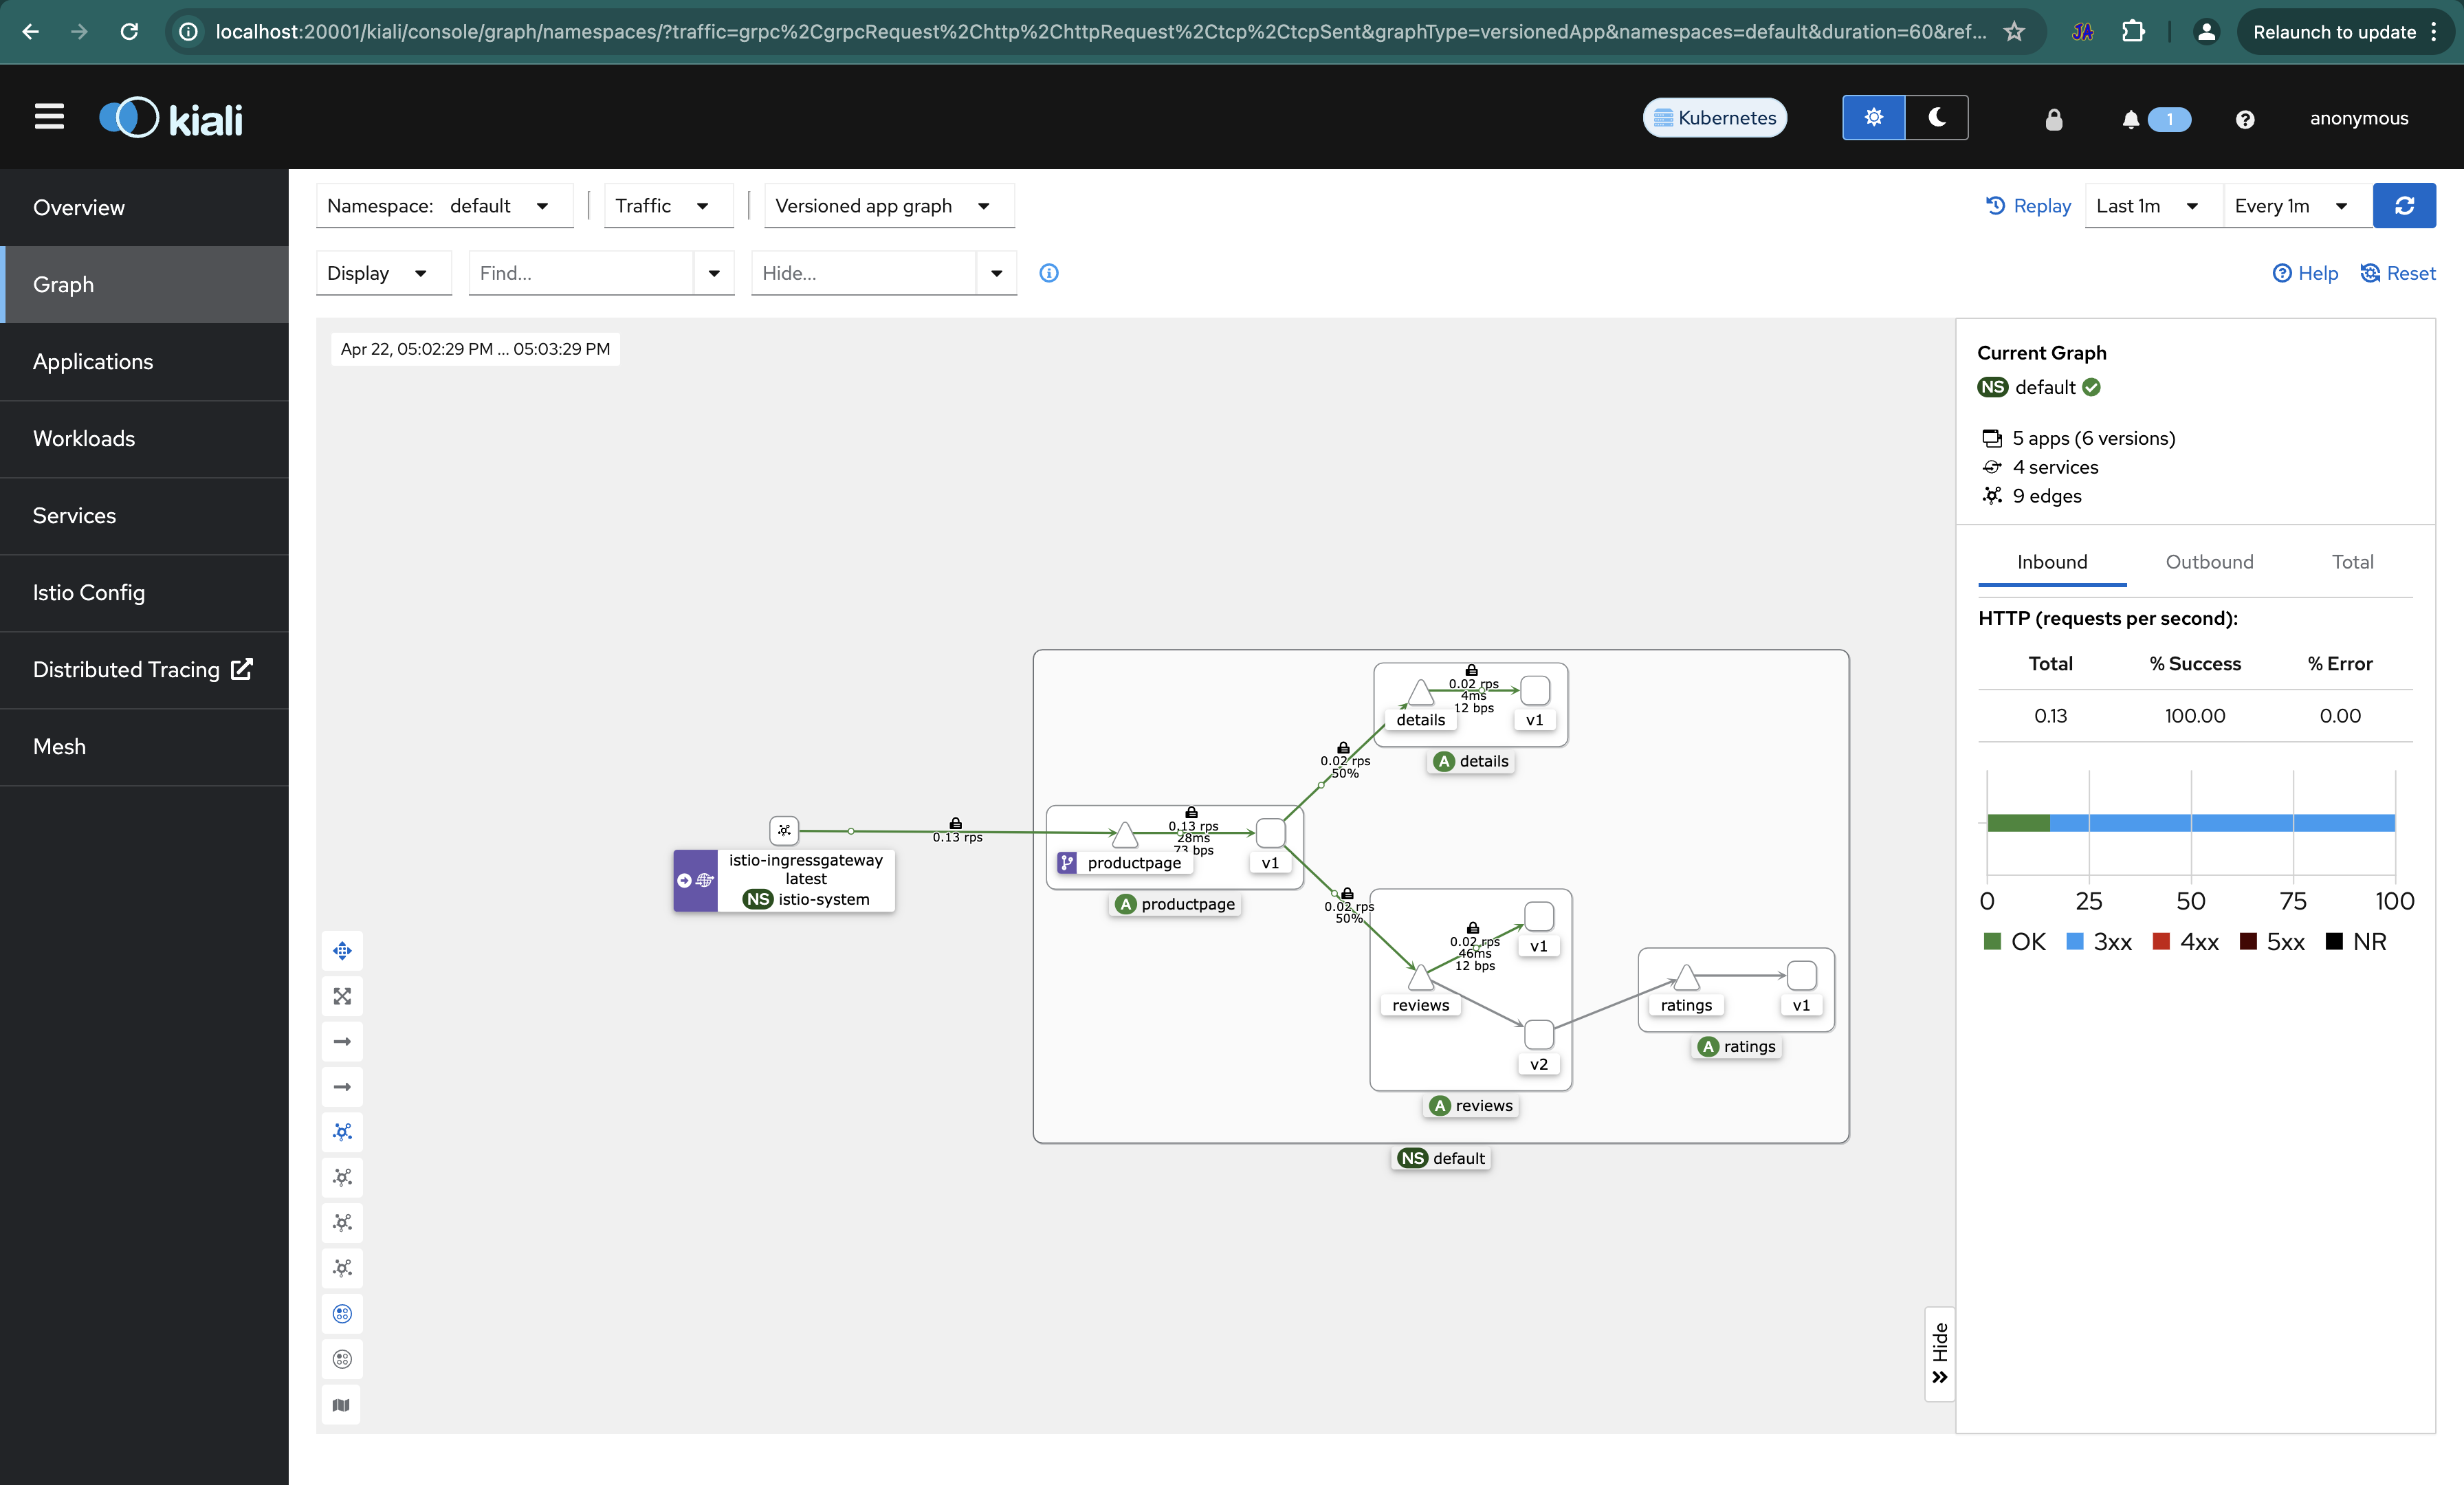
\includegraphics[width = \textwidth]{kailiConsole1.png} 
	\caption{Kaili Console} 
	\label{fig:kaili1} 
\end{figure}
\FloatBarrier

%%---------- Backmatter, referentielijst ---------------------------------------

\backmatter{}

\setlength\bibitemsep{2pt} %% Add Some space between the bibliograpy entries
\printbibliography

\end{document}
